\documentclass[11pt,a4paper]{book}

%$Id$

\usepackage{graphicx}

\usepackage{ifpdf}
\ifpdf
\usepackage{epstopdf}
\usepackage[usenames,dvipsnames]{color}
\usepackage[pdftex,bookmarks=true,hypertexnames=false]{hyperref}
\hypersetup{
  pdfauthor = {Jing Liu},
  pdftitle = {},
  pdfsubject = {PhD Thesis},
  pdfkeywords = {neutrino, double beta decay, germanium detector},
}
\pdfadjustspacing=1
\else
\usepackage[usenames,dvips]{color}
\fi

\usepackage{amsmath}            % more evironment
\usepackage{amssymb}            % more symbol

%\usepackage{fancyhdr}
%\fancyhead{}                    %clear default settings
%\fancyfoot{}                    %clear default settings
%\fancyhead[ER]{\rightmark}
%\fancyhead[EL]{\thepage}
%\fancyhead[OL]{\leftmark}
%\fancyhead[OR]{\thepage}

\setlength{\oddsidemargin}{1cm}
\setlength{\evensidemargin}{0cm}
\setlength{\textwidth}{15cm}
\setlength{\textheight}{21cm}
\setlength{\hoffset}{0cm}
\setlength{\voffset}{0cm}



%%% Local Variables:
%%% mode:latex
%%% TeX-master: "thesis"
%%% End:


\begin{document}

\pagestyle{empty}

\begin{titlepage}

\centering

\vspace{1.0cm}
\begin{figure}[t!]
\centering

\includegraphics[height=0.12\textheight]{TUM_logo}\hfil%
\begin{minipage}[b]{0.65\textwidth}\centering
\huge Technische Universit\"at M\"unchen\\\vspace{20pt}
\large \textit{Max-Planck-Institut f\"ur Physik\\
(Werner-Heisenberg-Institut)}
\end{minipage}\hfil%

\includegraphics[height=0.12\textheight]{MPP_logo}%
\end{figure}

\vspace{1. cm}

\huge Development of Segmented Germanium Detectors for Neutrinoless Double Beta Decay Experiments

\vspace{1.5 cm}

\Large Jing Liu

\vspace{2. cm}

\normalsize Vollst\"andiger Abdruck der von der Fakult\"at f\"ur
Physik der Technischen Universit\"at M\"unchen zur Erlangung des
akademischen Grades eines \\
Doktors der Naturwissenschaften (Dr. rer. nat.) \\
genehmigten Dissertation. \\

\vspace{1.5 cm} 

\begin{table*}[h]
  \centering
  \begin{tabular}{ll}
    Vorsitzender: & Univ.-Prof. xxx\\ 
    & \\ 
    Pr\"ufer der & 1. Hon.-Prof. Allen C. Caldwell, Ph.D \\ 
    Dissertation: & 2. Univ.-Prof. xxx \\ 
  \end{tabular}
\end{table*}

\vspace{2.0 cm} 

Die Dissertation wurde am xx.xx.2009 bei der Technischen Universit\"at
M\"unchen eingereicht und durch die Fakult\"at f\"ur Physik am
xx.xx.2009 angenommen. \\

\end{titlepage} 

%%% Local Variables:
%%% mode:latex
%%% TeX-master: "thesis"
%%% End:


\cleardoublepage

\section*{Abstract}
The results from neutrino oscillation experiments indicate that at least two neutrinos have mass. However, what the absolute mass scale of neutrinos is and whether neutrino and anti-neutrino are their own anti-particles remain unsolved. Neutrinoless double beta decay experiments can help to improve our understanding of both problems and are the most practical method known to tackle the second question. 

The GERmanium Detector Array (GERDA) experiment searching for the neutrinoless double beta decay of $^{76}$Ge is currently under construction in Hall A of the INFN Gran Sasso National Laboratory (LNGS), Italy. In order to achieve an extremely low background level, segmented germanium detectors will be operated directly in liquid argon which serves as cooling and shielding material simultaneously. 

Several test cryostats were built to operate segmented germanium detectors in vacuum and cryogenic liquid at the Max-Planck-Institut f\"ur Physik in M\"unchen, Germany. The performance and the background discrimination power of segmented germanium detectors were studied in detail. It was proved for the first time that the segmented germanium detector can be operated directly in cryogenic liquid stably for a long period, and that the segmentation scheme employed does well in the identification of photon and neutron induced background.

A comprehensive C++ simulation framework, MaGe (Majorana-Gerda), is jointly developed by the Majorana and GERDA collaborations. It is based on Geant4, but tailored to be especially suitable for the simulation of the response of ultra-low radioactive background radiation detectors to ionizing radiation. The predictions of the simulations were verified to hold to 5\%.

Pulse shape analysis is a complementary method to segmentation for further identifying background events. Its identification efficiency needs to be estimated using reliable pulse shape simulations. A full-functional pulse shape simulation package was developed within the MaGe framework. The simulation was verified using data taken from the first segmented prototype detector for GERDA. The understanding of the properties of the segmented germanium detectors was improved meanwhile.

\clearpage


\section*{Zusammenfassung}
(google translate version)

Die Ergebnisse von Neutrino-Oszillation Experimente deuten darauf hin, dass mindestens zwei Neutrinos Masse haben. Aber was die absolute Masse des Neutrinos Massstab ist und ob Neutrino und Anti-Neutrino sind ihre eigenen Anti-Teilchen nach wie vor ungel\"ost. Neutrinoless double beta decay Experimente zur Verbesserung unseres Verst\"andnisses der Probleme und sind die praktischste Methode, um die zweite Frage.

Die GERmanium Detector Array (GERDA) Experiment der Suche nach dem neutrinoless doppelte Beta-Zerfall von $^{76}$Ge ist derzeit im Aufbau in der Halle A des INFN Gran Sasso National Laboratory (LNGS), Italien. Um eine extrem niedrige Hintergrund Ebene, segmentierten Germanium-Detektoren werden direkt in fl\"ussigem Argon die als K\"uhl-und Abschirmmaterial gleichzeitig.

Mehrere Tests Kryostaten wurden f\"ur den Betrieb segmentierten Germanium-Detektoren im Vakuum und kryogene Fl\"ussigkeit auf dem Max-Planck-Institut f\"ur Physik in M\"unchen, Deutschland. Die Leistungsf\"ahigkeit und den Hintergrund der Diskriminierung Macht der segmentierten Germanium-Detektoren wurden im Detail untersucht. Es wurde bewiesen, für die das erste Mal, dass die segmentierten Germanium-Detektor kann direkt in kryogenen Fl\"ussigkeit stabil f\"ur eine lange Zeit, und dass die Segmentierung des Systems besch\"aftigt hat auch bei der Identifizierung von Photonen-und Neutronen-induzierten Hintergrund.

Eine umfassende C++-Framework, MaGe (Majorana-Gerda), wird gemeinsam von der Majorana und GERDA Kooperationen. Es basiert auf Geant4, aber abgestimmt auf die besonders geeignet für die Simulation der Reaktion der ultra-niedrige radioaktive Strahlung Hintergrund Detektoren durch ionisierende Strahlung. Die Vorhersagen der Simulationen wurden \"uberpr\"uft, um zu 5 \%.

Pulsform-Analyse ist eine erg\"anzende Methode zur Segmentierung für die weitere Ermittlung Hintergrund Veranstaltungen. Die Ermittlung der Effizienz muss anhand zuverl\"assiger Pulsform Simulationen. Eine vollst\"andige funktionelle Pulsform Simulation Paket wurde entwickelt, in der Magier Rahmen. Die Simulation wurde \"uberpr\"uft anhand der Daten aus den ersten Prototyp segmentierten Detektor f\"ur Gerda. Das Verst\"andnis f\"ur die Eigenschaften der segmentierten Germanium-Detektoren wurde inzwischen verbessert.

\clearpage

%%% Local Variables:
%%% mode:latex
%%% TeX-master: "thesis"
%%% End:


\cleardoublepage \setcounter{page}{1} \pagenumbering{Roman}

\tableofcontents

\cleardoublepage \setcounter{page}{1} \pagenumbering{arabic}

\pagestyle{headings}

\chapter{Introduction}
\label{cha:intro}
\addcontentsline{toc}{chapter}{Introduction}
\chapter*{Introduction}
\label{cha:intro}
At the time the \emph{Standard Model} was established the neutrino was believed to be massless. In experiments it always had the same chirality and there was no evidence for a non-zero mass. However, the picture changed dramatically when neutrino oscillations were observed in solar and atmospheric neutrinos. They were explained by the weak interaction eigenstates of neutrinos being admixture of mass eigenstates and the latter propagating with different velocities. The introduction of neutrino mass terms into the Standard Model became necessary.

There are various methods to introduce neutrino mass terms into the Standard Model. The most straightforward approach is to follow the same procedure as for the charged leptons, \textit{i.e.} the leptons obtain mass by coupling to the Higgs field. The problems of this approach are, that it does not explain why neutrinos couple to the Higgs field so weakly compared to their charged partners, and that it requires the introduction of right-handed neutrinos which have not yet been experimentally observed. An elegant way to solve these problems is to assume that neutrinos are Majorana particles, \textit{i.e.} their own anti-particles. This way, the second problem does not arise, and once the Majorana mass terms are introduced into the Lagrangian, the so-called \emph{see-saw mechanism} can make the different coupling strengths look natural.

Different theoretical and experimental methods are under investigation to verify that neutrinos are Majorana particles. The only experimental test currently possible is the search for the neutrinoless double beta ($0\nu\beta\beta$) decay. In this process, a neutrino emitted from one beta decay is absorbed by another beta decay. This can only occur, if neutrinos are of Majorana type. About ten naturally occurring isotopes are observed to undergo double-beta decay. Among them, $^{76}Ge$ is of special importance because germanium is a semiconductor material used in highly efficient detectors with very good energy resolution (it can serve as source and detector simultaneously), and it is the purest material produced in the world limiting intrinsic background.

The GERDA (GERmanium Detector Array) experiment \cite{Abt04, Sch05}, searching for the $0\nu\beta\beta$ decay of $^{76}Ge$, is currently under construction in Hall A of the INFN Gran Sasso National Laboratory (LNGS), Italy. In order to achieve an extremely low background level, the second phase of GERDA features 18-fold segmented germanium detectors operated directly in cryogenic liquid, serving as cooling and shielding material. The main goals of the work presented in this thesis are to examine systematically the operation and performance of segmented detectors in cryogenic liquid and to investigate their power of background discrimination by analyzing the spatial distribution over which energy is deposited. The time structure of the detector response is studied and simulated to lay the foundation for its use in background suppression.

Two test facilities were used to take data with two 18-fold segmented GERDA Phase~II prototype detectors:\\
\emph{Gerdalinchen~II}, a specially designed cryostat containing liquid nitrogen or argon, inside which up to three segmented detectors can be operated simultaneously. It was used 
\begin{itemize}
\item to operate and study for the first time segmented detectors submerged directly in cryogenic liquid.
\item to develop detailed operating procedures.
\item to carefully study the data of a prototype detector.
\end{itemize}
\emph{ A vacuum cryostat}, especially equipped to operate one segmented detector. It allowed
\begin{itemize}
\item the analysis of background induced by external photons in the MeV-energy range. These photons typically undergo multiple Compton scattering and deposit their energies over a range of several centimeters. This distinguishes them from the electrons from $0\nu\beta\beta$ decay which deposit energy on a millimeter scale.
\item the analysis of background induced by neutron interactions with germanium isotopes and surrounding materials. Most of the neutron induced events deposit their energies in different segments of the detector. Particularly, the inelastic scattering of neutrons at germanium isotopes can be identified through the separation of the energies deposited by the prompt photon and the nuclear recoil.
\item the characterization of the detector, including the segment boundaries, crystal axes and impurities, \textit{etc.}. The data was used to study the time structure of the detector response, \textit{i.e.} pulse shape and verify corresponding simulations. 
\end{itemize}

The test facilities were modeled using the a Geant4 based simulation framework, MaGe, which is jointly developed by the GERDA and Majorana collaborations. The measurements mentioned were simulated using MaGe. The simulation of low energy electrons, photons and neutrons interacting with germanium detectors and surrounding materials were verified in detail. A fully functional pulse shape simulation package was also developed within the MaGe framework. The whole signal formation process in segmented germanium detectors and the read-out system was simulated and verified by being compared with data. 

The thesis is structured as follows:
\begin{description}
\item[Chapter~\ref{cha:theory}] describes the theoretic background of $0\nu\beta\beta$ decay as well as other approaches to test whether neutrinos are of Majorana or Dirac type.
\item[Chapter~\ref{cha:exps}] summarizes different technical approaches of searching for $0\nu\beta\beta$ decays of different isotopes, compares the experiments with each other and estimates the potential of future $0\nu\beta\beta$ decay experiments.
\item[Chapter~\ref{cha:gerda}] introduces the basic ideas of the GERDA experiment, summarizes the latest progress, and estimates the potential of GERDA.
\item[Chapter~\ref{cha:detector}] describes the basic concepts of semiconductor detectors and the important properties of germanium crystals and detectors related to the later analysis.
\item[Chapter~\ref{cha:teststand}] introduces the two test stands that provided the data for all studies, describes the slow control and data acquisition system on which the test stands rely.
\item[Chapter~\ref{cha:GII}] characterizes the short and long term performance of segmented germanium detectors submerged in cryogenic liquid.
\item[Chapter~\ref{cha:np}] describes a special class of events with negative baseline shifts.
\item[Chapter~\ref{cha:photon}] demonstrates the power of segmented detectors to identify photon induced background and verifies the Monte Carlo simulation.
\item[Chapter~\ref{cha:neutron}] demonstrates the power of segmented detectors to identify neutron interactions with germanium isotopes and surrounding materials, validates the simulation in this aspect as well.
\item[Chapter~\ref{cha:pss}] describes the physics models of the charge carrier drift inside germanium detectors to simulate the pulse shape and introduces methods to add electronic effects.
\item[Chapter~\ref{cha:psa}] verifies the pulse shape simulation by comparing it to the data taken with the GERDA prototype detector and introduces new methods to determine the crystal orientation and impurity distributions.
\end{description}
The results are summarized within the context of the GERDA Phase~II experiment and an outlook to further studies is given.


%%% Local Variables:
%%% mode:latex
%%% TeX-master: "thesis"
%%% End:

\clearpage{\pagestyle{empty}\cleardoublepage}

\chapter{Neutrino mass}
\label{cha:theory}
%$Id$



%%% Local Variables:
%%% mode:latex
%%% TeX-master: "thesis"
%%% End:

\clearpage{\pagestyle{empty}\cleardoublepage}

\chapter{The GERDA experiment}
\label{cha:gerda}
The GERDA (GERmanium Detector Array) experiment~\cite{Sch05} is designed to search for $0\nu\beta\beta$ decay of $^{76}$Ge. The main design feature is to operate naked germanium detectors directly in liquid argon in order to achieve extremely low background level. The concept is based on ideas presented in Ref~\cite{Heu95}. Detailed introduction of the experiment can be found in the first section of this chapter. GERDA is currently under construction in Hall A of the INFN Gran Sasso National Laboratory (LNGS), Italy. The current status of the experiment is described in the second section. The development of GERDA is divided into three phases. In the first phase (Phase I) unsegmented germanium detectors, which were previously used in IGEX~\cite{Aal02} and HdM~\cite{Hei04} experiments, will be re-deployed. The envisioned background level is $10^{-2}$~events/(kg$\cdot$keV$\cdot$year). In the second phase (Phase II) 18-fold segmented detectors, which currently are under construction, will be used in addition. The aimed background level is $10^{-3}$~events/(kg$\cdot$keV$\cdot$year). A later phase (Phase III) is under discussion in cooperation with the MAJORANA Collaboration~\cite{Gai03,Aal04} aiming at a one tonne scale experiment. The physics observation capabilities of three phases of GERDA are discussed in the last section.

\section{Concept}
\label{sec:gerda:conc}
The germanium detector has been used to detect ionizing radiation, particularly X-rays and $\gamma$-rays for years. It has energy resolution better than 1\% around the $Q$-value region of the $0\nu\beta\beta$ decay, which is among the bests in all $0\nu\beta\beta$ decay detectors introduced in Sec.~\ref{sec:gencon}. This provides very good separation of $0\nu\beta\beta$ decay signal from $2\nu\beta\beta$ decay background. However, the natural abundance of $^{76}$Ge (7.6\%) is not very high, hence additional enrichment is needed. And the $Q$-value of the $0\nu\beta\beta$ decay of $^{76}$Ge, 2.039~MeV, is still lower than some of the natural radiation lines. Special designs are needed to reduce the background. Fig.~\ref{fig:gerda} shows the engineering drawing of the structure of GERDA. Each part of the structure is introduced in the following sections as well as its functionality of reducing background from different sources.

\begin{figure}[tbhp]
  \centering
  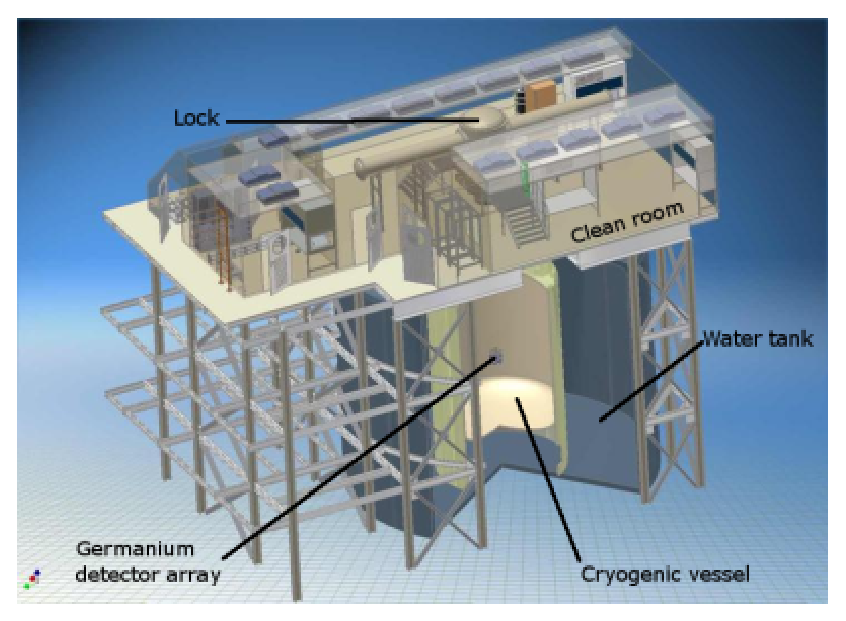
\includegraphics[width=0.7\textwidth]{gerda}  
  \caption{Structure of GERDA from engineer's view.}
  \label{fig:gerda}
\end{figure}

\subsection{Location and muon veto}
\label{sec:gerda:loca}
In order to reduce the cosmic ray induced background GERDA was chosen to be located in Hall A of the INFN Gran Sasso National Laboratory (LNGS), Italy. LNGS is the largest underground facility in the world for low-background experiments. It can be accessed from a 10~km long highway tunnel under the Gran Sasso mountains. It has three experimental halls hosting a large variety of experiments, most of which focus on dark matter or neutrino physics. Fig.~\ref{fig:lngs} shows the location of GERDA in LNGS. The main experimental site of GERDA is between the Large Volume Detector (LVD) and a service tunnel across Hall A. The GERDA auxiliary and cryogenic storage system will be located in the service tunnel on the northeast side of Hall A.

\begin{figure}[tbhp]
  \centering
  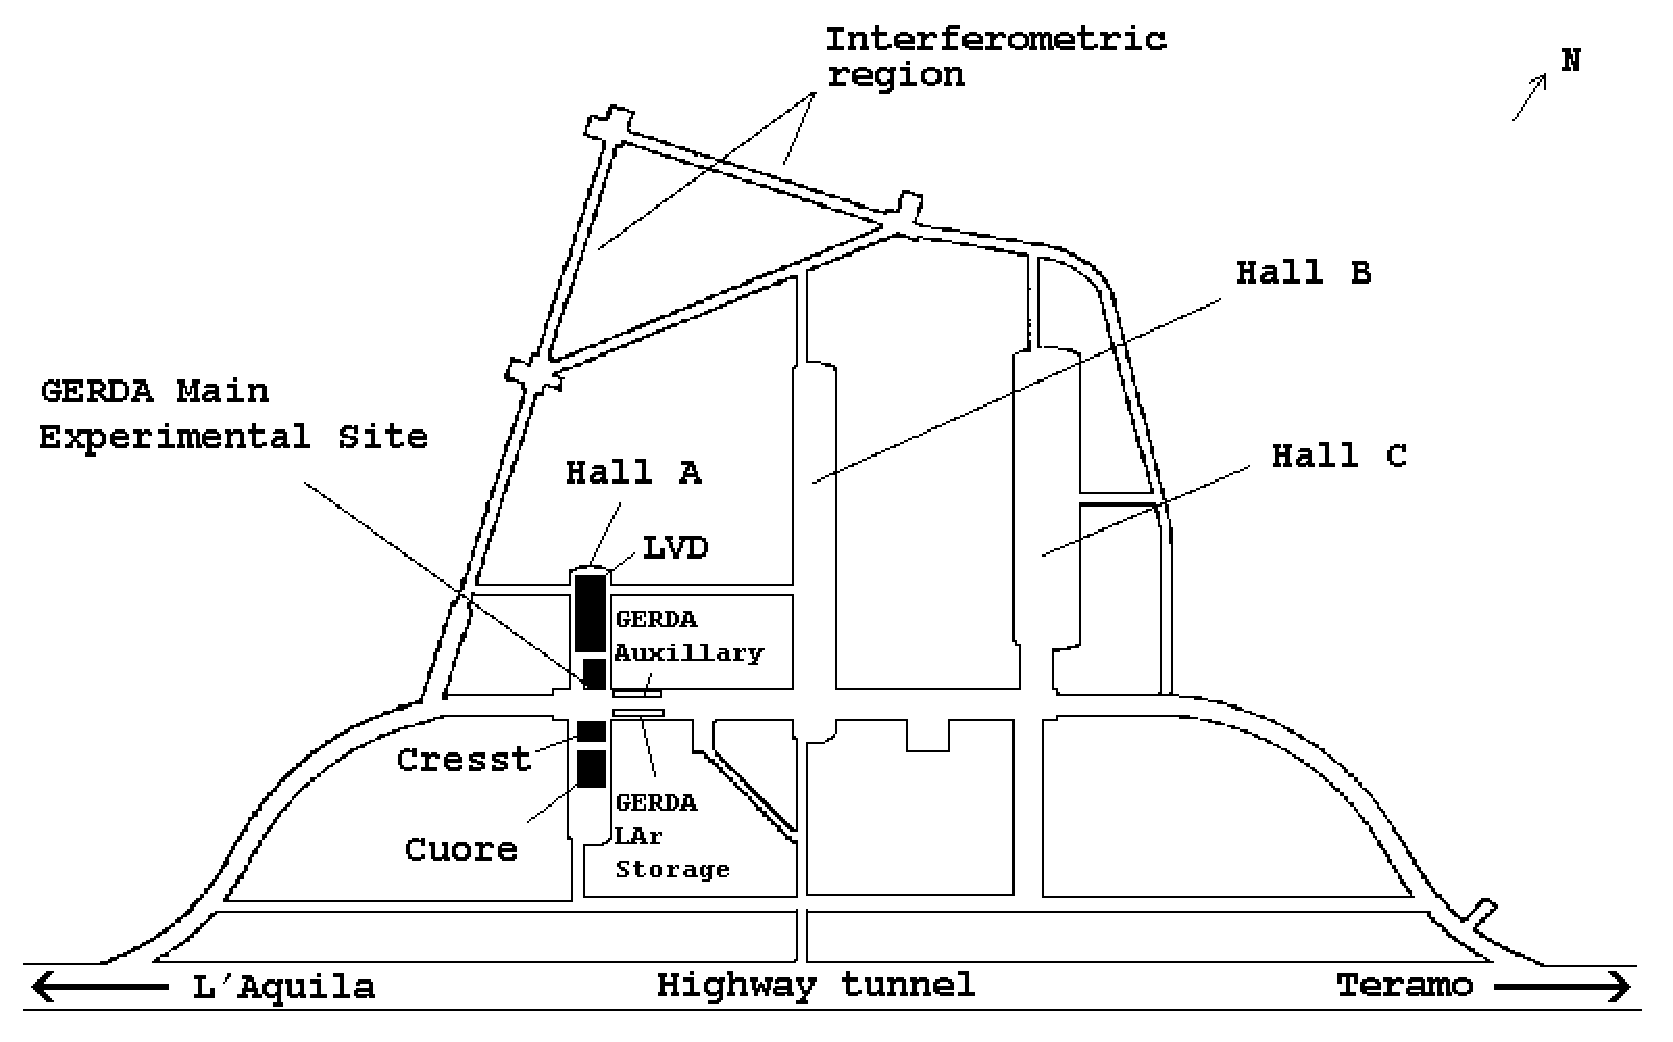
\includegraphics[width=0.8\textwidth]{lngs}  
  \caption{Location of GERDA in LNGS. The main experimental site of     GERDA is between the Large Volume Detector (LVD) and a service     tunnel across Hall A. The GERDA auxiliary and cryogenic storage     system will be located in the service tunnel on the northeast side     of Hall A.}
  \label{fig:lngs}
\end{figure}

The overburden of 1.4~km of rock on top of the experimental halls corresponds to 3.4~km meter of water equivalent (m.w.e). It reduces the cosmic ray induced muon flux by a factor of $10^{6}$, and neutron flux a factor of $10^{3}$ compared to the surface. The energy and angular distribution of cosmic ray muons in Hall A of LNGS have been precisely measured~\cite{Amb95, Lip91, Amb03}. A comprehensive study of cosmic ray induced muon and neutron background in underground laboratories can be found in Ref.~\cite{Mei06}.

In order to further reduce the muon induced background additional muon veto system will be implemented. Cosmic muons traversing the water buffer will cause Cherenkov radiation. To detect the radiation 66 photomultiplier tubes (PMTs) will be installed on the walls of the water tank. The positions of PMTs are optimized according to Monte Carlo simulation. Together with these PMTs the water tank could be operated as a Cherenkov detector. The detection efficiency is about 95\% depending on the incident angle of the muon. In order to compensate for the missing water volume around the neck of the cryostat plastic scintillator plates will be placed on top of the clean room. They are used to detect the muons entering the cryostat almost vertically. The combined detection efficiency is expected to be above 99\%.

\subsection{Water tank and cryostat}
\label{sec:gerda:rock}
To mediate and absorb the neutron radiation from the rock $\sim 630$~m$^{3}$ of ultra-pure water will be filled in a stainless steel tank with an outer diameter of 10~m and a height of about 8~m. Since liquid argon can be produced with a much greater purity than lead or even copper traditionally used for shielding, a total of approximately 98~t of liquid argon will be stored in a cryostat placed inside the water tank to shield $\gamma$-rays from the rock and water. The vessel is made of stainless steel with an internal copper liner. The height of the vessel is 5.88~m (7.62~m with the neck) while the outer diameter is 4.16~m.

\subsection{Detector suspension system and electronics}
\label{sec:gerda:cable}
Germanium detectors will be suspended in liquid argon from the top of the cryostat. In order to minimize the contamination from the suspension system, signal and high voltage cables light-weighted detector holding frames and novel contacting scheme shown in the left plot of Fig.~\ref{fig:array} will be used. The frames are made of thin ultra-pure copper bars with a total weight of about 30~g. They will be chained vertically into strings. Each string consists of 3 detectors with the same type, as shown in the middle plot of Fig.~\ref{fig:array}. The whole detector array could maximally consists of 16 hexagonally packed detector strings as shown in the right plots of Fig.~\ref{fig:array}. 

The horizontal distance between the centers of two detectors is 9~cm. The vertical clearance between two detectors is about 6~cm. The Phase I detectors are p-type diodes with a cylindrical closed-ended coaxial geometry. The detectors are enriched in $^{76}$Ge to a level of about 86\% and have masses between 0.9~kg and 2.9~kg. The detectors for Phase II will be cylindrical true coaxial n-type diodes. The precise size of the detectors will depend on manufacturing details. The most likely dimensions are a height of 70~mm and a diameter of 75~mm. The detectors will be segmented. The segmentation scheme under consideration is a 6-fold segmentation in the azimuthal angle $\phi$ and a 3-fold segmentation in the height z. 

\begin{figure}[tbhp]
  \centering
  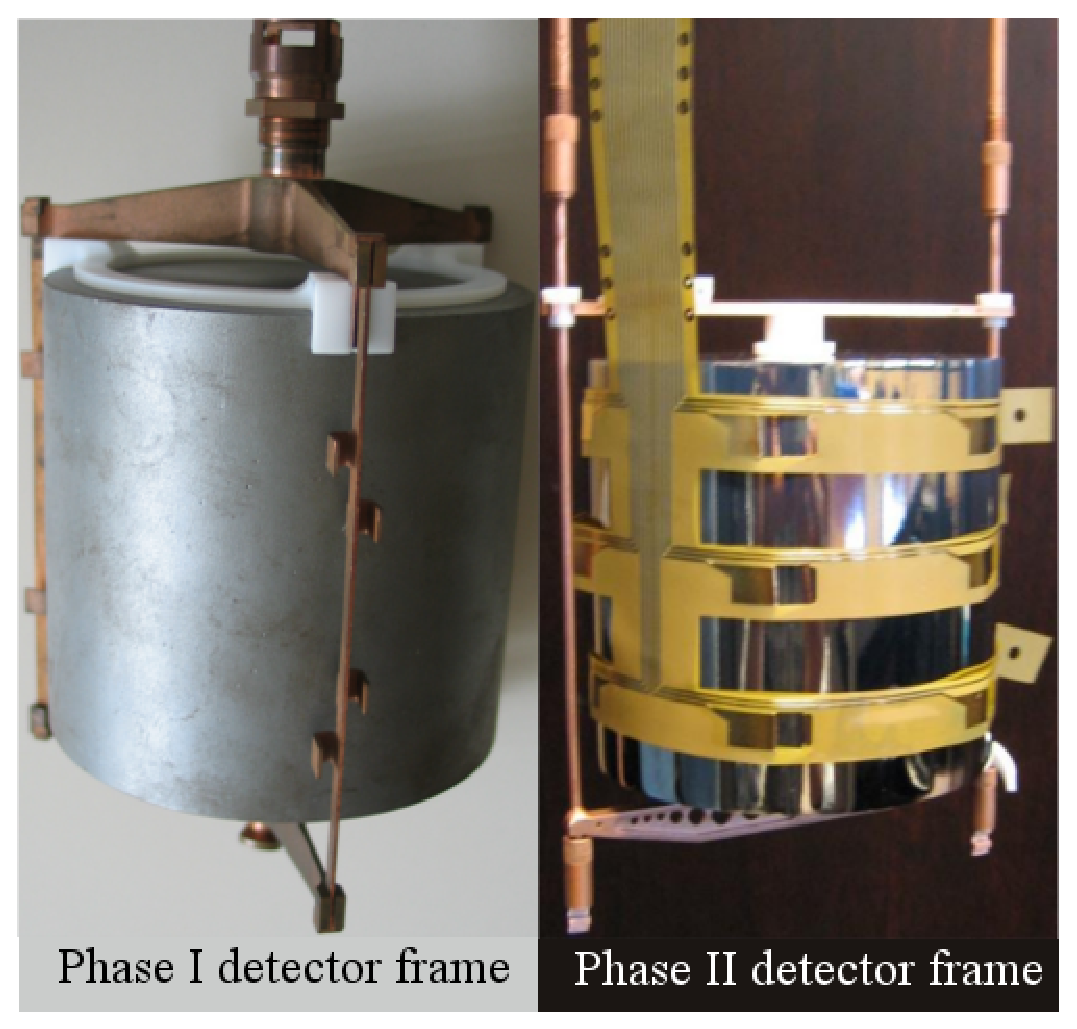
\includegraphics[width=0.33\textwidth]{detectorFrame}
  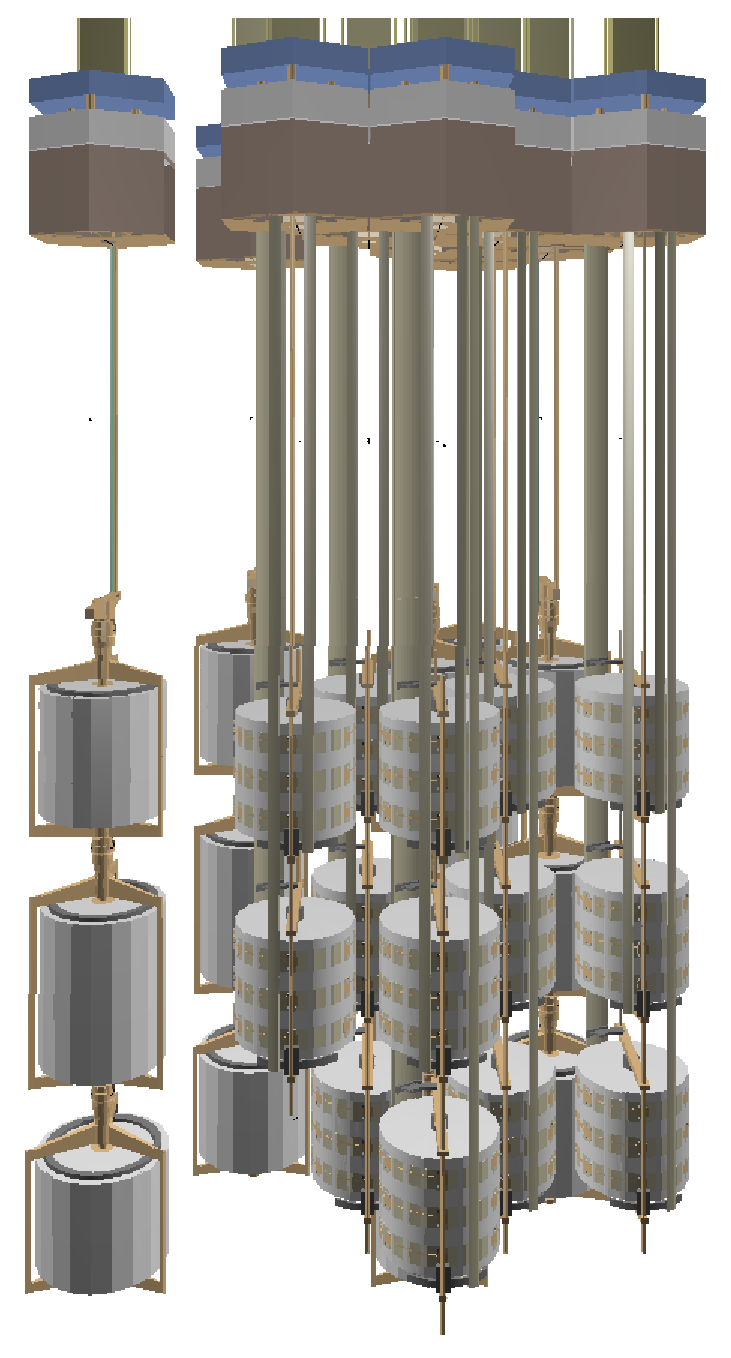
\includegraphics[width=0.2\textwidth]{array}   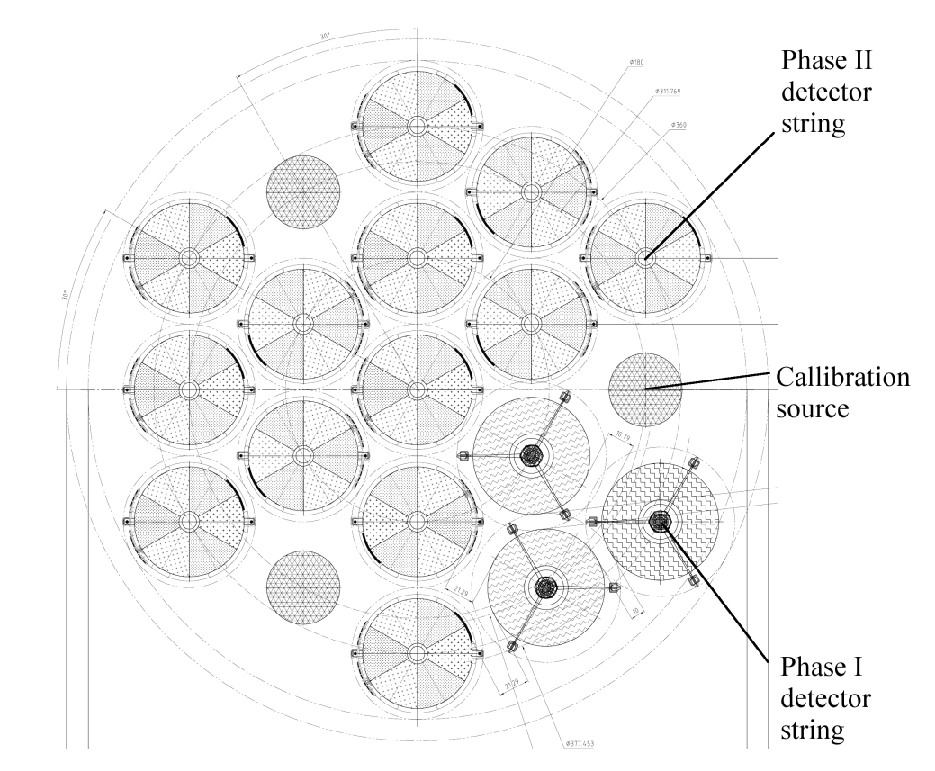
\includegraphics[width=0.45\textwidth]{arrayTop}
  \caption{Detector array configuration. The left plot shows single     Phase I detector with copper frame and Phase II detector with     copper frame and a novel contacting scheme. The middle plot shows     how the detectors are chained into strings and hung together in     liquid argon.  The right plot shows the top view of the full array     indicating the possible positions for the Phase I and Phase II     detector strings as well as for the calibration sources.}
  \label{fig:array}
\end{figure}

A couple of solutions are actively pursued for the read-out electronics of GERDA~\cite{Cat07}. A common scheme foresees a cold FET close to the crystal followed by amplifying and load driving circuits located at room temperature. The cold FET would be placed near the connection matrix (top blocks in the middle plot of Fig.~\ref{fig:array}) 30~cm above the detector array. Pre-amplified signals would be sent to circuits at room temperature through 6~m long cables, as this is the minimum distance from crystal to room temperature environment.

\subsection{Detector storage and clean room}
\label{sec:gerda:source}
When processed or transfered above ground, germanium detectors are exposed to cosmic radiation and radioactive isotopes could be produced inside the detector through spallation caused by energetic cosmic rays. Two cosmogenic isotopes, $^{60}$Co and $^{68}$Ge, have Q-values above that of $^{76}$Ge $0\nu\beta\beta$ decay and are potential sources of background. Therefore the detector processing time above ground needs to be minimized. Since the half life time of $^{60}$Co and $^{68}$Ge is 5.3 years and 271 days, respectively, a passive method to reduce their contamination is to wait long enough so that most of them decay.

When exposed to the air, germanium detector surface may be contaminated by dust which contains many radioactive isotopes undergoing $\alpha$ decay. The detector surface is not fully charge sensitive and only part of the energy lost by the $\alpha$ particle can be detected. This may result in a signal close to the $Q$-value of $^{76}$Ge $0\nu\beta\beta$ decay. Therefore the testing, preparation and insertion of the detector need to be done in a rather clean environment. For this purpose, a class 10000 clean room with radon-reduced air will be built on top of the cryostat. It houses a lock through which detector strings are inserted into and removed from the cryogenic volume. Detector handling will be performed in flow-boxes and a detector mounting station which will reach class 100.  The lock consists of a rail system which allows to move detector strings into their correct position and lower them into the cryostat. In addition, the clean room will be used to temporarily store germanium detectors under a controlled atmosphere of gaseous argon as shown in Fig.~\ref{fig:store}.

\begin{figure}[tbhp]
  \centering
  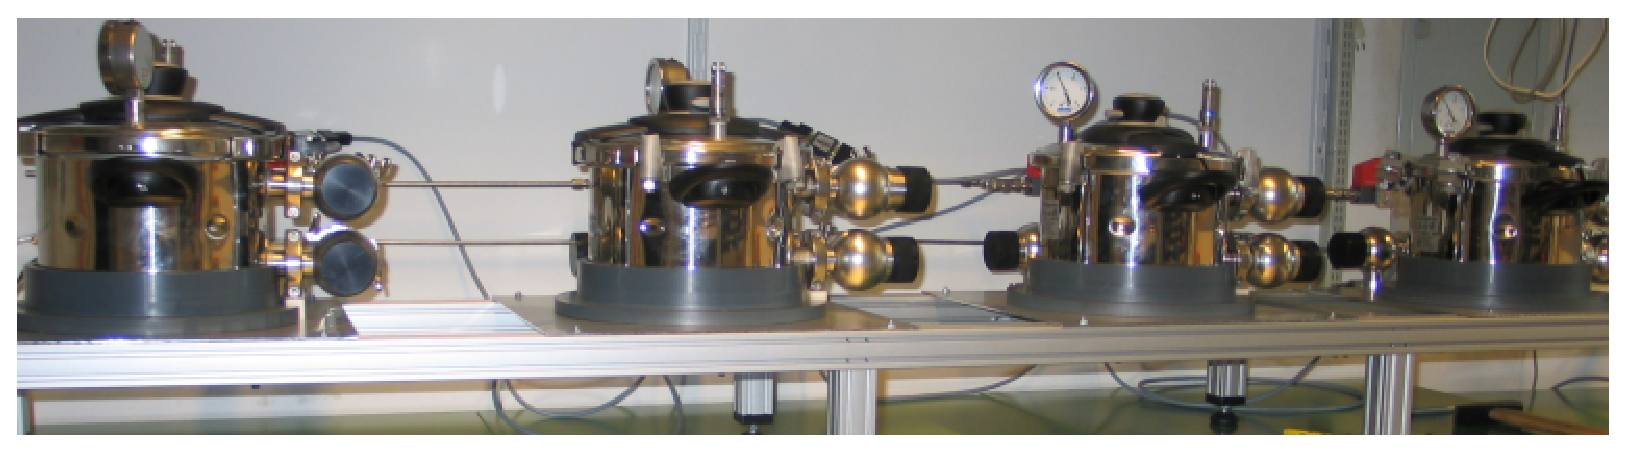
\includegraphics[width=\textwidth]{storage}
  \caption{Detector storage system. The left plot shows an open vacuum     can with a detector inside. The middle plot shows a closed vacuum     can equipped with valves and gas flux sensor. The right plot shows     four vacuum cans connected with gas tubes.}
  \label{fig:store}
\end{figure}

\subsection{Other background rejection techniques}
\label{sec:gerda:anti}
Other background rejection techniques that can be used in GERDA include 1. anti-coincidence measurement, 2. pulse shape analysis, and 3. instrumentation of the cryostat.
\begin{description}
\item[Anti-coincidence] Compton-scattered photons are likely to   deposit energy in more than one detector while $0\nu\beta\beta$   decay electrons will predominantly deposit energy in only one   detector. Photons can thus be identified by requiring more than one   detector to see energy above the threshold. Considering the   segmented detectors for Phase II photons depositing energy in one   crystal can still be identified by requiring more than one segment   to show energy. Time anti-coincidence veto could also be used to   reject background induced by the decay of $^{68}$Ge and $^{77}$Ge   meta stable state. Feasibility studies are currently carried out.
\item[Pulse shape analysis] Although photons are likely to create more   than one energy deposition, if these energy depositions are confined   to one segment, the anti-coincidence between segments cannot   distinguish this kind of event from $0\nu\beta\beta$ decay signal.   However, by analyzing the time structure of the detector response,   \textit{i.e.} pulse shape, photons and electrons can be further   distinguished~\cite{Kev07}.
\item[instrumentation of the cryostat] Liquid argon scintillates if   energy is deposited inside the argon volume. The scintillation light   can be detected by PMT's mounted on the walls of the cryostat.   Events with photons in the final state which deposit only a fraction   of their energy inside the germanium detectors can be vetoed by   requiring an anti-coincidence between the observed scintillation   light and the energy deposit inside the detectors.  This technique   is not part of the GERDA baseline design. Feasibility studies are   currently being performed~\cite{Pei05, Orr06}.
\end{description}

\section{Status}
\label{sec:gerda:stat}
This section closes with the status of GERDA as of Winter 2008/09. Important milestones and results are summarized below.  

\subsection{Cryostat and water tank}
\label{sec:gerda:stat1}
On 6 March 2008, the cryostat was delivered to LNGS and placed at the foreseen location in Hall A, as shown in the middle plot of Fig.~\ref{fig:cryo}. Mounting of the internal copper shield was completed on March 18. The cryostat passed several acceptance tests including pressure tests, helium leak tests, liquid nitrogen evaporation tests and radon emanation measurements. The water tank installation finished at the end of June, as shown in the right plot of Fig.~\ref{fig:cryo}. The installation of the cryostat and water tank with the design specifications is a major milestone for GERDA.

\begin{figure}[tbhp]
  \centering
  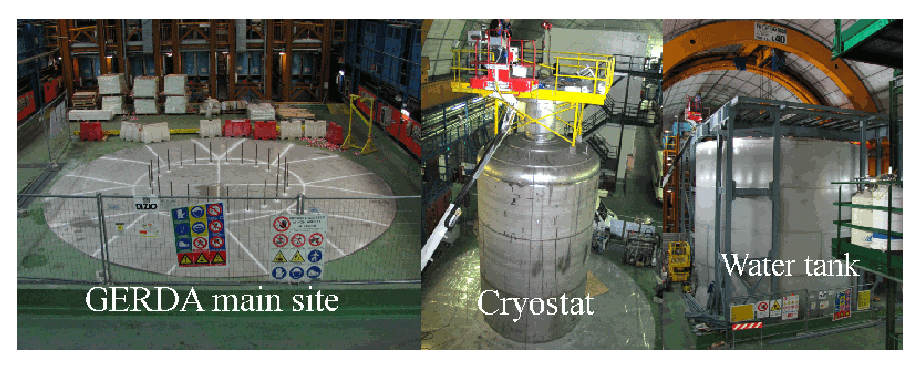
\includegraphics[width=\textwidth]{cryostat}
  \caption{Construction of cryostat and water tank in GERDA main site.     From left to right: the empty GERDA main site, the installed     cryostat and water tank and some infrastructure around it.}
  \label{fig:cryo}
\end{figure}

\subsection{Clean room and lock system}
\label{sec:gerda:stat2}
As shown in the right plot of Fig.~\ref{fig:cryo}, the construction of the infrastructure around the water tank is ongoing, on top of which the clean room and lock will be erected. The design of the clean room is finished. The construction is scheduled to finish at February 2009. The design of the complete lock structure is almost finished. The lock will be preinstalled at the Max-Planck-Institut f\"ur Physik in Munich and then transported to LNGS early 2009. A provisional lock system is in production. It will be used before the complete lock system is ready so that the commissioning of GERDA could start at February 2009.

\subsection{Phase I and II detectors}
\label{sec:gerda:stat3}
In total 17.9~kg of enriched and 15~kg of non-enriched high-purity p-type germanium detectors from IGEX, HdM and Genius Test Facility (GTF)~\cite{Kla02} will be operated in Phase I of GERDA.  Stability tests of the operation of p-type detectors in cryogenic liquids are practically completed.  After two years of operation with more than 50 warming and cooling cycles, the $\gamma$-ray induced leakage current has been proved to be negligible if the passivation layer is limited to the groove area only, and the detector handling procedure has been defined.

In total 14 segmented germanium detector, each weighs 1.62~kg, will be used for GERDA Phase II. 37.5~kg enriched germanium dioxide, which will be used to produce Phase II detectors is stored in the HADES underground facility. The yield for the purification of GeO$_{2}$ to 6N metal is about 90\% and the time above ground for the purification will not exceed 2 to 3 days. The crystal will be grown in the Institut f\"ur Kristallz\"uchtung (IKZ) in Berlin. Small crystals from zone-refined material with the concentration of impurities between $10^{12}$ and $10^{11}$ per cm$^{3}$ has been pulled in IKZ, as shown in Fig.~\ref{fig:pulling}. The Czochralski puller has been refurbished already set up to produce 2~inch crystals.
\begin{figure}[tbhp]
  \centering
  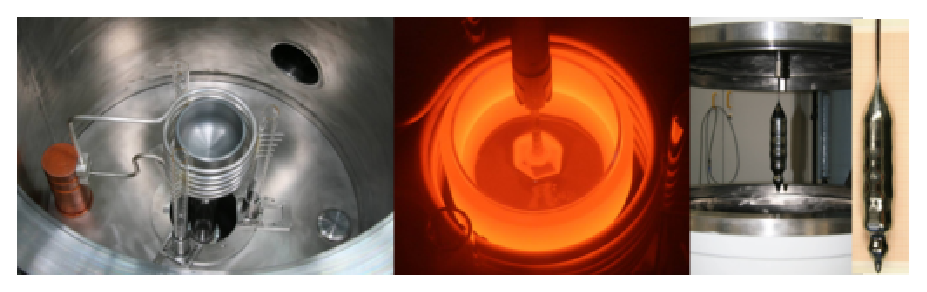
\includegraphics[width=\textwidth]{crystalPulling}
  \caption{Pulling crystal in Czochralski puller. From left to right: Czochralski puller, pulling crystal, pulled crystal and a close look of it.}
  \label{fig:pulling}
\end{figure}

The first Phase II prototype detector operated in a conventional cryostat has been tested and characterized~\cite{Sie07}. The second prototype detector has been equipped with the novel signal contacts and operated in liquid nitrogen for months. The handling, operating and testing of the prototype detectors and the physics analysis based on the data from them are the main topics of this thesis and will be discussed in detail in the following chapters.


\subsection{Other progress}
\label{sec:gerda:stat4}
Front-End electronics has been tested in liquid nitrogen with two new detector test stands, namely, Sub with a p-type detector and Gerdella with an n-type detector. Measurements with Sub gave an energy resolution of 2.6~keV (FWHM) at 1.3~MeV. Optimization in terms of noise performance is ongoing and further improvements expected.

As for muon veto system, a batch of 10 plastic scintillator panels has been assembled at Dubna and tested in LNGS. The tests have shown that the concept works. And the PMT production has successfully completed. 

The behavior of radon and its daughters in liquid nitrogen has been studied. It has been proved that radon would not be taken away by boiled-off nitrogen and stays predominantly in the liquid, and that radon, in particular its progenies $^{214}$Po and $^{218}$Po are attracted to steel plates if either positive or negative high voltage is applied. Measurements in argon and with germanium substrates are now under preparation. This effect, if it persists in LAr/Ge, would offer the possibility to remove actively residual radon traces by implementing electrodes to sweep out radon and their progenies. 


\section{Sensitivity}
\label{sec:gerda:sens}
A dedicated discussion about the sensitivity of GERDA can be found
in Ref.~\cite{Cal06}. The left plot in Fig.~\ref{fig:gerda:limit}
taken from Ref.~\cite{Cal06} shows the expected 90\% probability lower
limit on the half lifetime for $0\nu\beta\beta$ decay versus the
exposure under different background conditions. Also shown is the half
lifetime for the claimed observation by H. V. Klapdor-Kleingrothaus
\textit{et al.}~\cite{Hei04}. The right plot shows the expected 90\%
probability upper limit on the effective Majorana neutrino mass versus
the exposure under different background conditions. The effective
Majorana neutrino mass for the claimed observation is also shown. All
mass values are determined from the half lifetime using the matrix
element reported in Ref~\cite{Rod07}.
\begin{figure}[tbhp]
  \centering
  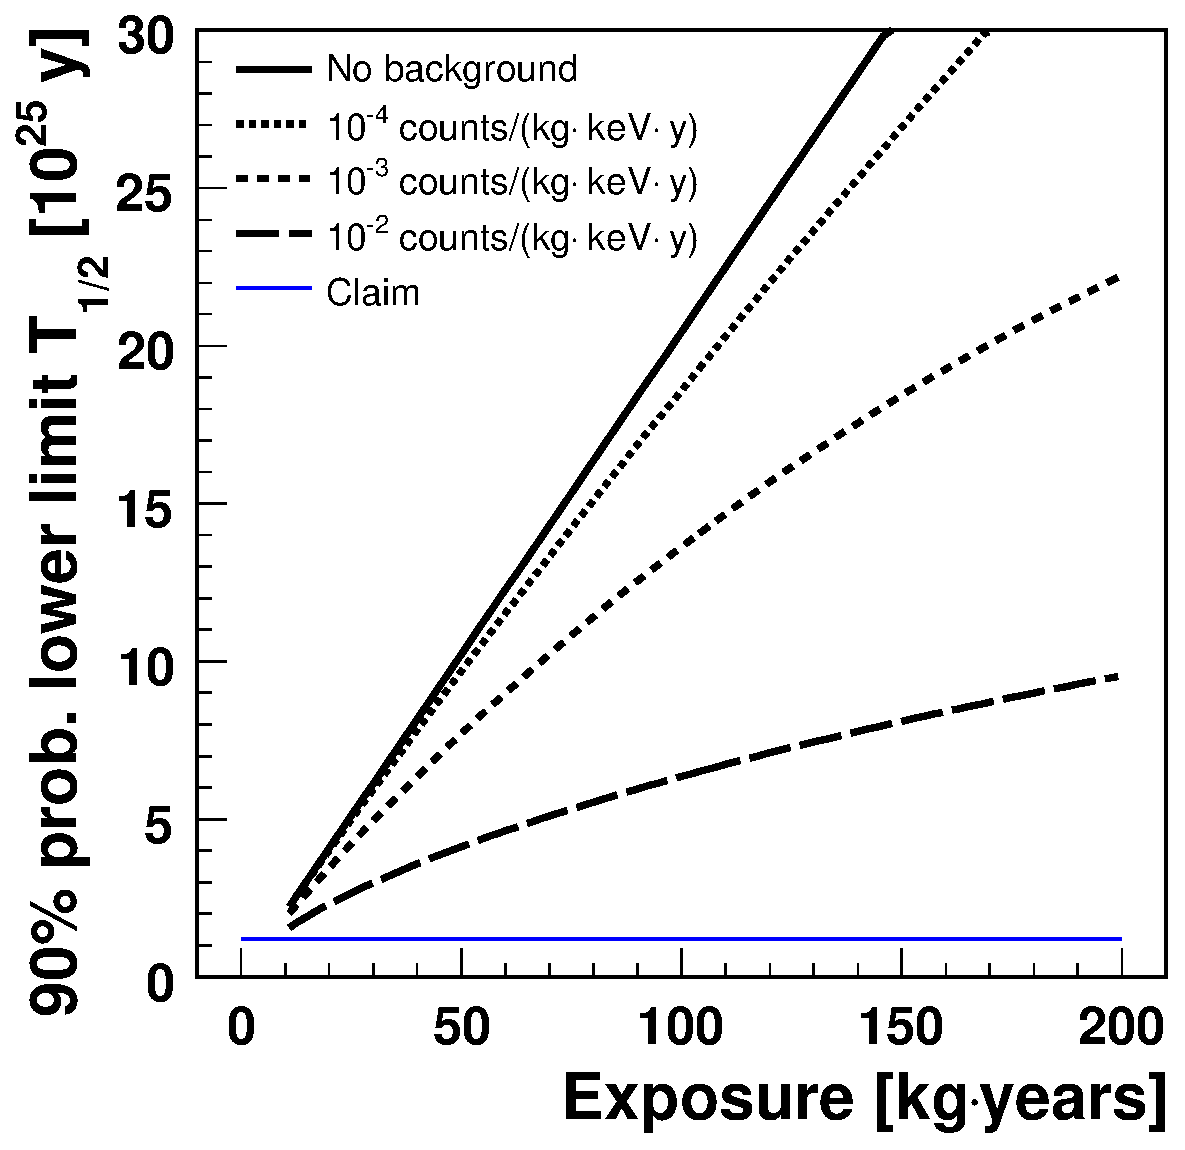
\includegraphics[width=0.45\textwidth]{limit_halflife}  \hfil
  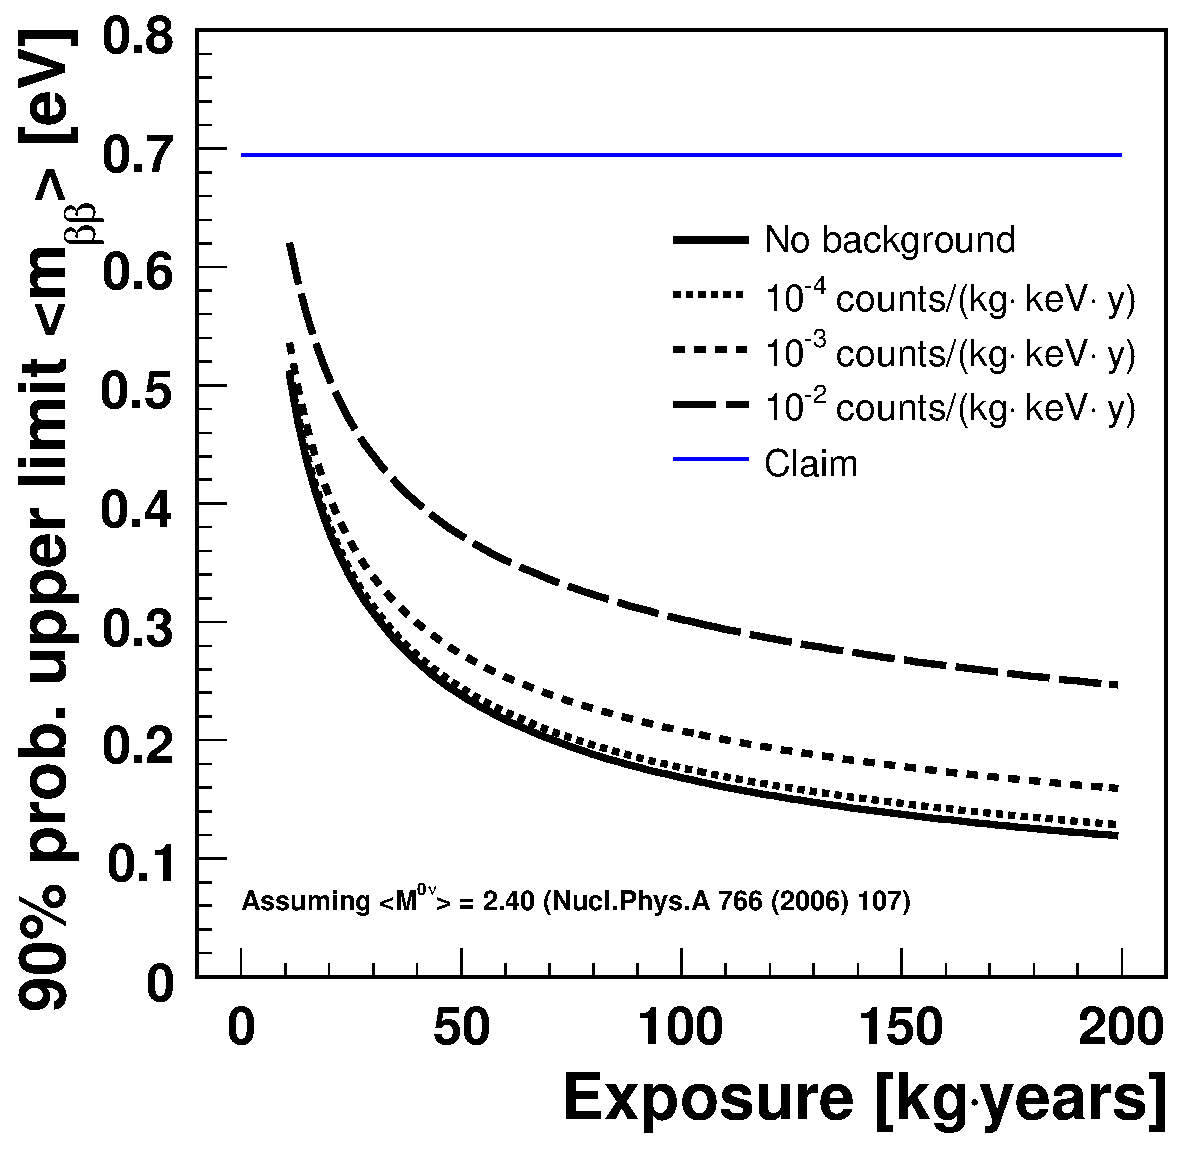
\includegraphics[width=0.45\textwidth]{limit_mass}
  \caption{The expected 90\% probability lower limit on the half    
lifetime for $0\nu\beta\beta$ decay (left) and the expected 90\%    
probability upper limit on the effective Majorana neutrino mass    
(right) versus the exposure under different background conditions.    
Also shown is the half lifetime and the effective Majorana    
neutrino mass for the claimed observation by H. V.    
Klapdor-Kleingrothaus \textit{et al.}~\cite{Hei04}. All mass    
values are determined from the half lifetime using the matrix    
element reported in Ref~\cite{Rod07}.}
  \label{fig:gerda:limit}
\end{figure}

For GERDA Phase I, assuming a background level of $10^{-2}$~events/(kg$\cdot$keV$\cdot$year) and an exposure of
100~(kg$\cdot$year), an upper limit on $m_{\beta\beta}$ of
0.3~eV would be achievable. For Phase II, assuming a background level of $10^{-3}$~events/(kg$\cdot$keV$\cdot$year) and an exposure of
100~(kg$\cdot$year), an upper limit on $m_{\beta\beta}$ of
0.2~eV would be achievable.


%%% Local Variables:
%%% mode:latex
%%% TeX-master: "thesis"
%%% End:

\clearpage{\pagestyle{empty}\cleardoublepage}

\chapter{Germanium detectors}
\label{cha:detector}
\chapter{Signal formation in germanium detectors}
\label{cha:detector}
When particles ($\alpha, \beta, \gamma, n, p$, etc.) interact inside
the germanium semiconductor detector, they create electron-hole pairs,
which act as charge carriers. Due to the electric field inside the
detector the charge carriers drift and induce electric signals in
electrodes. The electric signals are amplified, digitized and recorded
by the electronics and data acquisition systems connected to the
germanium detector. The whole process of signal formation in germanium
detectors and their supporting electronics is briefly reviewed in this
chapter.

\section{Interactions of radiation with matter}
\label{sec:det:phys}

\subsection{Electrons and positrons}
\label{sec:det:ep}
Electrons and positrons traversing matter lose their kinetic energy
mainly by two processes, ionization and bremsstrahlung. High energy
(GeV range) electrons and positrons predominantly lose energy by
bremsstrahlung. Low energy (MeV range) electrons and positrons
predominantly lose energy by ionization. The energy at which an
electron or a positron loses as much energy in collisions as in
radiation is called critical energy $\epsilon$. For elements with
charge $Z > 13$ the critical energy is \cite{Ama81}
\begin{equation}
\label{eq:det:ecrit}
\epsilon = (550/Z) \text{ MeV}.
\end{equation}
For germanium $\epsilon \approx 17$~MeV. Hence, electrons emitted from
the double beta decay of $^{76}$Ge mainly loss their energy by
ionization.

The range of electrons and positrons depends on their energy and the
material they traverse (see Ref.~\cite{Bri84} and references
therein). The average range of a 1~MeV electron in germanium is about
0.5~mm.

After a positron has lost all its kinetic energy, it annihilates with
an electron into two photons with an energy of 511~keV each,
corresponding to the rest mass of electrons.

\subsection{Photons}
\label{sec:det:gamma}
Photons emitted by radioactive isotopes have energies ranging from
several keV to several MeV. The possible interaction processes of
photons in matter are photoelectric effect, Compton (incoherent)
scattering, Rayleigh (coherent) scattering and pair production. Since
Rayleigh scattering does not change the energy of the scattered photon
but only its momentum, it is not relevant for GERDA.

\textbf{Photoelectric effect:} When a photon interacts with an atom,
its entire energy may be transferred to an atomic shell electron which
leaves the shell. The energy of the secondary electron is equal to the
difference of the incident photon energy and the binding energy of the
electron. If the electron originates from an inner shell of the atom,
an outer shell electron fills the vacancy. Consequently, either
characteristic x-rays are emitted, or, if the x-ray photons are
re-absorbed, secondary Auger-electrons are emitted. The cross section
of the photoelectric effect is inversely proportional to the photon
energy. Hence, the photoelectric effect is the main interaction
mechanism for photons at low energy (up to about 200~keV for Ge).

\textbf{Compton scattering:} A photon scatters on a weakly bound
electron (quasi-free), transferring only part of its energy and
momentum. The angular distribution of the scattered photons is
described by the Kein-Nishina formula. The maximum energy transfer
occurs when the incident photon is scattered by $180^{\circ}$. Compton
scattering is the predominant interaction process for photons of
energies between about 200~keV and 8~MeV for germanium. A 1.33~MeV
photon undergoes on average three Compton scatterings before being
absorbed through the photoelectric effect. The mean free path of such
a photon is about three centimeters.

\textbf{Pair production:} If the photon energy exceeds twice the rest
mass of the electron, the photon can create an electron-positron pair
in the electric field of a nucleus. The rest of the photon energy is
transferred to the created electron and positron as kinetic energy. A
significant cross section for this interaction mechanism arises only
for energies above $4\sim5$~MeV.

\subsection{Neutrons}
\label{sec:det:neutron}
Because of the lack of charge, neutrons have a relatively high
penetration power. However, there are five processes that occur when
neutrons interact with nuclei depending on the kinetic energy of the
incident neutrons:

\textbf{Capture:} The nucleus, Z, absorbs the incident neutron, $n$,
and de-excites with the emission of one or more photons, denoted as
$^{\text{A}}$Z$(n,\gamma)$, where A is the atomic number of the
nucleus. In case of \textbf{internal conversion} an electron from a
lower shell of the nucleus is emitted instead of a photon, denoted as
$^{\text{A}}$Z$(n,e)$. The excited nucleus can also be meta-stable and
not de-excite instantaneously, denoted as
$^{\text{A}}$Z$(n,\gamma^{m})$. Capture is the dominant process for
thermal neutrons, \textup{i.e.}, neutrons with energies in the sub-eV
range.

\textbf{Elastic scattering:} A neutron collides with a nucleus,
transfers some energy to it and bounces off in a different direction;
the target nucleus gains the energy lost by the neutron (also called
recoil energy). This is one of the significant processes for neutrons
with energies in the range of keV to several tens of MeV. The recoil
energy is very small (mostly less than 200~keV) and has an
exponentially decaying distribution. Hence, this process is not
relevant as a background for $0\nu\beta\beta$ decay searches.

\textbf{Inelastic scattering:} A nucleus temporarily absorbs the
incident neutron and forms a compound nucleus in an excited state. It
then de-excites by emitting another neutron of lower energy together
with a photon which takes the de-excitation energy. The nucleus takes
some recoil energy. The reaction is denoted as
$^{\text{A}}$Z$(n,n^{\prime}\gamma)$ and is significant for neutrons
with energies in the range of 1 to several tens of MeV.

\textbf{Transmutation:} A nucleus absorbs a neutron and then
de-energizes by emitting a proton, $p$, or an $\alpha$ particle. This
produces a nucleus of a different element. The process can occur when
the incident neutron energy exceeds $\approx 100$~MeV and becomes
dominant at several GeV.

If the neutron energy is even higher, fission reactions occur. Such
high energy neutrons can only be produced by cosmic ray muons which
are vetoed by the muon detecting system in GERDA. However, the
meta-stable nuclei created by such neutrons could be a serious
background for the $0\nu\beta\beta$ decay search (see
Sec.\ref{sec:gerda:santi}).


\section{Germanium detectors}
\label{sec:det:semi}

\subsection{Working principle of semiconductor detectors}
\label{sec:det:prin}
Insulators, semiconductors and conductors are distinguished according
to the energy gap between the valence and the conduction bands. The
widths of the band gap of semiconductors are between those of
insulators and conductors and are of the order of several~eV. This
allows an electron to be lifted from the valence to the conduction
band by thermal motion or external ionizing radiation.

The resistivity of a semiconductor is determined by impurities
(dopant) in its crystal lattice. Elements with only three valence
electrons create energy states a little bit higher than the valence
band, making it easy to lift valence electrons to these states and
create freely moving holes in the valence band. This kind of dopant is
called acceptor. The semiconductor doped with them is called
$p$-doped. Elements with five valence electrons donate electrons to
energy states a little bit lower than the conduction band, making it
easy to lift these weakly bound electrons to the conduction band. This
kind of dopant is called donor. The semiconductor doped with them is
called $n$-doped. In general, the thermal energy available at room
temperature is sufficient to ionize most of the dopant. The created
freely moving electrons and holes are called charge carriers.

A $p$-$n$ junction forms when $p$- and $n$-doped pieces of
semiconductor are placed together. The charge carriers diffuse into
regions with lower concentrations and are eliminated by
recombination. Left behind are the charged ions adjacent to the
interface in a region with no mobile carriers, called the
\emph{depletion zone}. Since these ions create positive space charges
on the $n$ side and negative ones on the $p$ side, an electric field
is created providing a force opposing the continued diffusion of
charge carriers. The size of the depletion zone changes when an
external potential is applied to the junction. Under \emph{reverse
bias} (anode connected to the $n$ side, cathode to the $p$ side) the
majority charge carriers are driven away from the junction. This
widens the depletion zone. Since the carrier density is small in the
depletion zone, only a very small reverse saturation current
occurs. Likewise, the depletion zone squeezes under \emph{forward
bias} while the current strongly increases.

The depletion zone is the active volume of any semiconductor
detector. When ionizing radiation strikes the depletion zone, some of
its deposited energy excites electrons out of the valence band and
electron-hole pairs are created. Due to the electric field
electron-hole pairs cannot recombine but split and drift towards the
electrodes and induce electric signals there. In most of the cases a
reverse bias is applied in order to create an active volume as large
as possible. The bias voltage turning the whole bulk of a
semiconductor detector into a depletion zone is called the full
depletion voltage.

\subsection{Operating voltage of germanium detectors}
\label{sec:det:volt}
The depletion depth is proportional to the square root of the ratio of
the applied voltage and the dopant concentration. The fewer dopants,
the bigger the depleted region under a certain reverse bias. The
concentration of active impurities in germanium detectors is of the
order of $10^{10}$/cm$^{3}$. Germanium has about $10^{22}$ atoms per
cm$^{3}$. The dopant concentration in germanium detectors is thus of
the order of 1~ppt (particle per trillion) which is extremely
low. Consequently, the depletion voltages of germanium detectors are
two orders of magnitude lower than for silicon detectors of the same
size. This allows the construction of large germanium detectors
operating at relatively low voltage. The largest germanium detectors
are based on a cylindrical geometry with diameter and height both in
the several centimeter range. The full depletion voltage for them is
just several kilo-volts. The operating voltage is normally a little
bit above the full depletion voltage to ensure a regular electric
field.

\subsection{Operating temperature of germanium detectors}
\label{sec:det:temp}
The smaller the band gap, the higher the probability that an electron
is transferred to the conduction band. The band gap in germanium is
0.72~eV, in silicon it is 1.1~eV. At room temperature the population
of electrons in the conduction band in germanium is a factor of 1000
higher than in silicon. Applying a bias voltage to a germanium
detector with a large bulk (about several cm) at room temperature
would create a large current. This would make the operation
impossible\footnote{The large bulk current creates a large noise
distorting any signal.}, or even destroy the detector. Germanium
detectors are usually cooled via a metal cooling stick submerged in a
cooling medium, \textit{e.g.}, liquid nitrogen, to suppress thermal
excitation.\footnote{The number of thermally excited electrons could
be very small when the germanium volume becomes small. Germanium
pieces thinner than several microns are used to make room temperature
detectors. No high voltage is needed to create the depletion zone. The
leakage current is very small. The noise from the thermal excitation
also becomes tolerable given very few thermally excited electrons.}
Due to imperfect heat conduction the temperature of the germanium
crystal is slightly higher than that of the cooling medium.

\subsection{Types of germanium detectors}
\label{sec:det:type}
Germanium detectors are naturally divided into two classes
characterized by the active impurities in the bulk material. If the
impurities are mainly acceptors, the material is $p$-doped and the
detector is called $p$-type. If the impurities are mainly donors, the
material is $n$-doped and the detector is called $n$-type.

Large germanium detectors normally have a cylindrical shape. They can
be divided into two types: \textit{true coaxial} and
\textit{closed-ended coaxial}. In both cases the shape is cylindrical
with an inner bore.\footnote{There are also some germanium detectors
having no hole in the middle. All the contacts are on the surface.}
For true coaxial detectors the core is completely removed, whereas for
the closed-ended coaxial geometry the core is only partially removed
leaving a \textit{cap} on one side.

The outer surface layer of a $p$-type detector is normally converted
into $n$-type with a typical thickness of about 0.5~mm by diffusing
lithium. It is sometimes classified as a \textit{dead layer}, because
the charge carriers created in this layer cannot be detected. The
inner surface of a $p$-type detector is implanted with boron in order
to make good electric contact. The thickness of the implantation is of
the order of several microns. $n$-type detectors have the lithium
drifted zone and thus the dead layer on the inner surface. Hence they
have less inactive volume. The boron implantation is on the outside.

Germanium detectors can also be classified as segmented or
unsegmented. The segmentation is normally performed on the outer
surface of the detector. For $p$-type detectors the outer surface is
milled in order to penetrate the thick lithium-drifted layer. The
fringe depths and thicknesses of the segments are of the order of a
millimeter. Distortions in the electric field are expected in this
case. For $n$-type detectors photo-lithographic techniques are used to
form the segments. The electric field is expected to be quite
homogeneous.

\section{Charge carriers}
\label{sec:det:drift}

\subsection{Creation of charge carriers}
\label{sec:det:exit}
A big fraction of the energy deposited by incident radiation causes
the excitation of phonons, the rest excites electrons from the valence
band to the conduction band. Thus, the average energy needed to create
one electron-hole pair, called pair energy, is much bigger than the
band gap. In germanium the pair energy is 2.95~eV at 80~K.

\subsection{Electric field and carrier drift}
\label{sec:det:field}
The reverse bias applied to the electrodes creates an electric field
in the bulk of the germanium detector which lets the charge carriers
drift to the electrodes. The field $\mathbf{E}$ is determined by the
boundary conditions as well as the space charges in the depletion
zone. It can be calculated by solving Poisson's equation:
\begin{equation} 
\label{eq:det:ef}
\nabla \cdot \mathbf{E} = \frac{\rho}{\epsilon},  
\end{equation}
where $\rho$ is the space charge density defined by the effective
number of impurities and $\epsilon$ is the dielectric constant.

\subsection{Effects of crystal structure}
\label{sec:det:struc}
The relation between the drift velocity of the charge carriers,
$\mathbf{v}_{e/h}(\mathbf{r})$, and the electric field,
$\mathbf{E}(\mathbf{r})$ can be simply expressed as:
\begin{equation} 
\label{eq:det:dv}
\mathbf{v}_{e/h} (\mathbf{r})= \mu_{e/h} \mathbf{E}(\mathbf{r}),
\end{equation}
where $\mu_{e/h}$ is called the \emph{mobility} and $\mathbf{r}$
indicates the position. In germanium detectors operating at low
temperatures the mobility is influenced by the crystal lattice
orientation and taking a complex form instead of a number. The drift
velocities along different directions differ from each other
(longitudinal anisotropy) and are not always parallel to the electric
field (transverse anisotropy). The angle between the drift direction
and the electric field is known as the Sasaki angle\cite{Sas56}. A
detailed discussion of the effects of the crystal structure on the
charge carrier drift is formed in Chapter~\ref{cha:pss}.

\section{Induction of signals in detector electrodes}
\label{sec:det:ramo}
Electric signals are induced in the electrodes of a detector by the
cumulative influence of electrons and holes moving toward the
electrodes. Shockley-Ramo's Theorem \cite{Gat82, Rad88, He00} can be
used to calculate the time development of the induced charge $Q(t)$ or
current $I(t)$ in each electrode:
\begin{equation} 
\label{eq:det:ramoq}
Q(t) = -Q_{0} \times [\varphi_{w}(\mathbf{r}_{h}(t)) -
\varphi_{w}(\mathbf{r}_{e}(t))],
\end{equation}
\begin{equation} 
\label{eq:det:ramoi}
I(t) = Q_{0} \times [\mathbf{E}_{w}(\mathbf{r}_{h}(t)) \cdot 
\mathbf{v}_{h}(t) - \mathbf{E}_{w}(\mathbf{r}_{e}(t)) \cdot 
\mathbf{v}_{e}(t)],
\end{equation}
where $Q_{0}$ is the electric charge carried by electrons or holes,
$\mathbf{r}_{e/h}(t)$ and $\mathbf{v}_{e/h}(t)$ are the position and
velocity vectors of electrons/holes as a function of time, and
$\varphi_{w}(\mathbf{r})$ and $\mathbf{E}_{w}(\mathbf{r})$ are the
so-called \emph{weighting potentials} and \emph{weighting
fields}. They can be calculated by solving Poisson's equations,
$\nabla^{2} \varphi(\mathbf{r}) = 0$ and $\nabla \cdot
\mathbf{E}(\mathbf{r}) = 0$, with the boundary condition that the
potential on the electrode of interest equals to 1 and the potentials
on all other electrodes equal to zero.

Figure~\ref{fig:det:psh} shows the weighting potential of a segment
with the indication of an event for the cross section at the center of
a Siegfried-like detector. Figure~\ref{fig:det:pss} shows the raw
charge and current pulses induced by the resulting hit in this
particular segment, its neighboring segments and the core of the
detector. The pulses induced in the neighboring segments are called
\emph{mirror pulses}. The amplitude of the mirror pulse induced in one
neighboring segment is larger than in the other, because the
trajectory of the hit is closer to this segment.
\begin{figure}[htbp] 
\centering 
\subfloat[]{\label{fig:det:psh} 
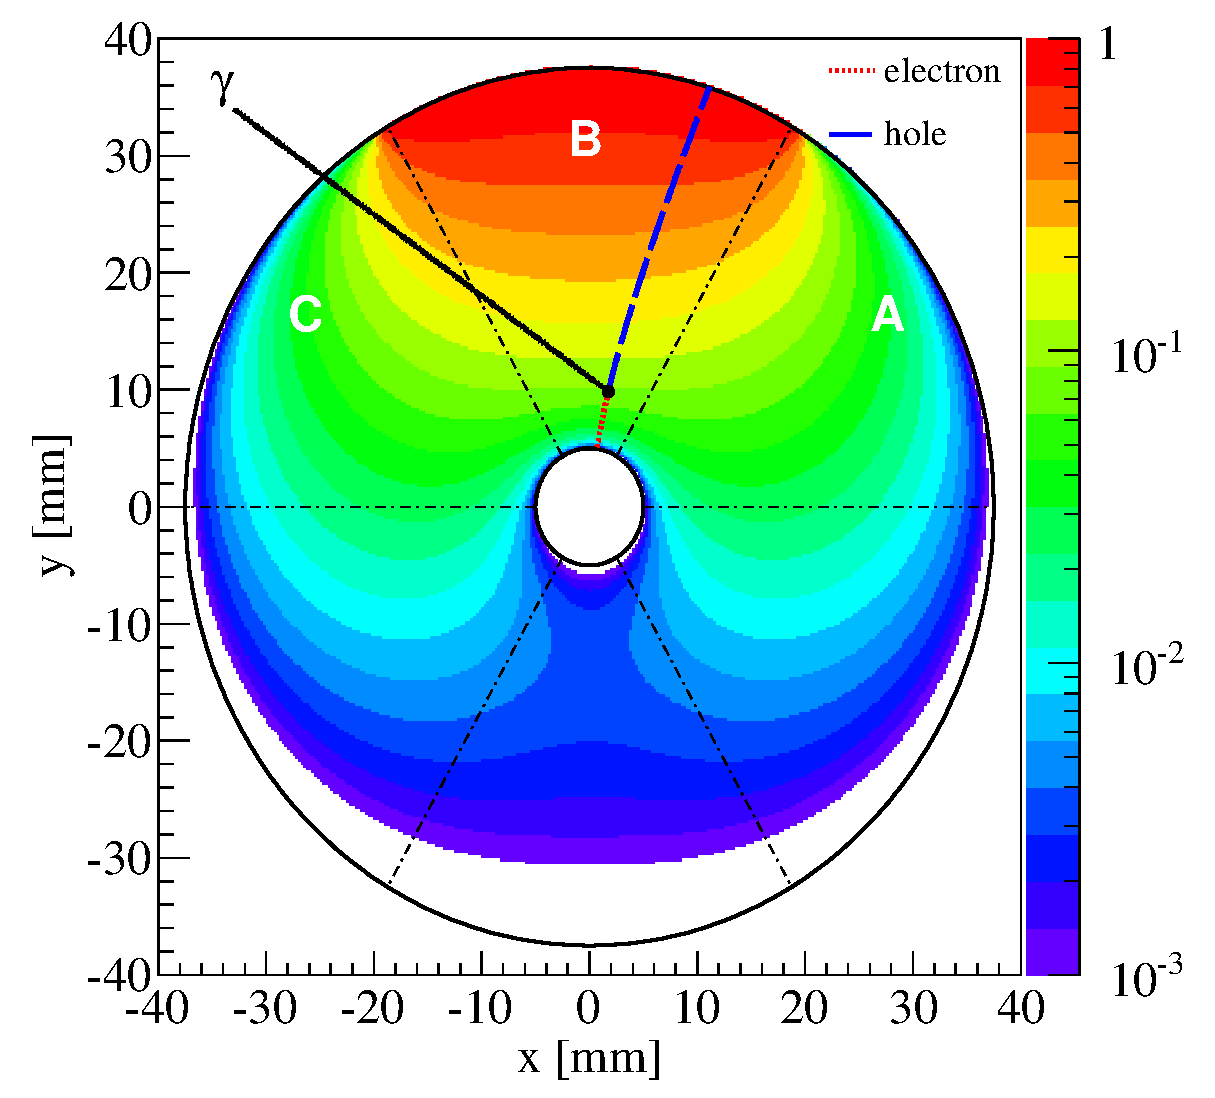
\includegraphics[height=0.22\textheight]{WP}}% 
\subfloat[]{\label{fig:det:pss} 
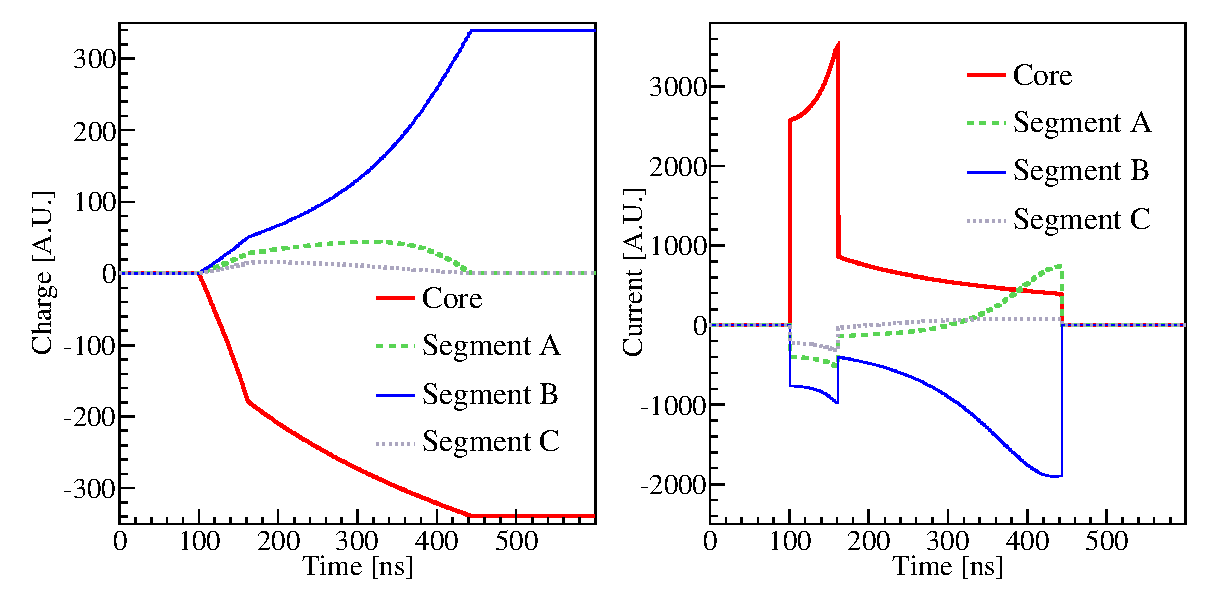
\includegraphics[height=0.22\textheight]{CIPS}}% 
\caption{(a) weighting potential of segment B together with an
indication of a $\gamma$ interaction. (b) Simulated charge and current
pulses induced in segments A, B and C.}
\label{fig:pss:ps} 
\end{figure} 

\section{Electronics}
\label{sec:det:elec}

\subsection{Noise}
\label{sec:det:noise}
The total energy resolution in terms of the full width at half maximum
(FWHM) of the peak under study, $W_{T}$, is composed of three terms:
\begin{equation}
W_{T}^{2} = W_{D}^{2} + W_{X}^{2} + W_{E}^{2},
\end{equation}
where $W_{D}$ describes the statistical fluctuations of the creation
of electron-hole pairs, $W_{X}$ describes the effect of incomplete
charge collection and scales linearly with the incident energy, and
$W_{E}$ accounts for noise contributions from the electronics and does
not depend on energy. Given a perfect electronic system, germanium
detectors have an energy resolution of about 2~keV at 1.3~MeV, where
$W_{X}$ dominates the contribution and $W_{D}$ contributes less than
1~keV. These two contributions cannot be reduced. In reality, thermal
noise in the pre-amplifiers and noise picked up by the cables and
connectors contribute significantly to the total noise. These
contributions have to be kept as small as possible.

\subsection{Cross talk}
\label{sec:det:xtalk}
For segmented germanium detectors, signals from all the electrodes are
read out simultaneously. There is intrinsic cross talk between
different channels because of the capacitive couplings between
electrodes. This cross talk is not due to improper electric
connections, hence cannot be avoided. However, it can be reduced to
an acceptable level by choosing proper values of resistors and
capacitors used in the pre-amplifier coupling and feed-back circuits
to match the intrinsic capacities between detector electrodes. A
detailed analysis is found in Chapter 4 of Ref.~\cite{Bru06} and
references therein.

%%% Local Variables:
%%% mode:latex
%%% TeX-master: "thesis"
%%% End:

\clearpage{\pagestyle{empty}\cleardoublepage}

\chapter{Munich test stands}
\label{cha:teststand}
Several test facilities at the Max-Planck-Institut f\"ur Physik, Munich, were developed for research and development of segmented $n$-type germanium detectors like the ones to be used in the Phase~II of the GERDA experiment. The operation and performance of several segmented detectors in vacuum and submerged in cryogenic liquid were systematically examined; various data samples were taken to investigate the event discrimination power of segmented germanium detectors. The test facilities are briefly discussed in this chapter. The data studies and analysis based on them are described in the following chapters.

\section{Cryostats}
\label{sec:tt:cryo}

\subsection{Dewar with vacuum can}
\label{sec:tt:comc}
Canberra-France developed a test cryostat shown in Fig.~\ref{fig:tt:comcryo}. A standard liquid nitrogen dewar is complemented by a two-walled aluminum vacuum can with a combined thickness of 6~mm. The detector was placed inside the can and the coordinate system was chosen such that its center was at $z=66$~mm and $r=0$~mm. The vacuum can extended to $z=116$~mm and $r=75$~mm. A copper cooling finger was used as a thermal link between the detector and the dewar. The temperature was monitored at several locations using Pt100 resistors. Liquid nitrogen was refilled daily maintaining a temperature stability of about $\pm3$~K. A comparison of spectra taken at different temperatures within this range showed neither significant differences in the general shape of the spectra nor in the energy resolution.

\begin{figure}[tbhp] 
  \centering 
  \subfloat[Dewar with vacuum can on top]{\label{fig:tt:dpc}
    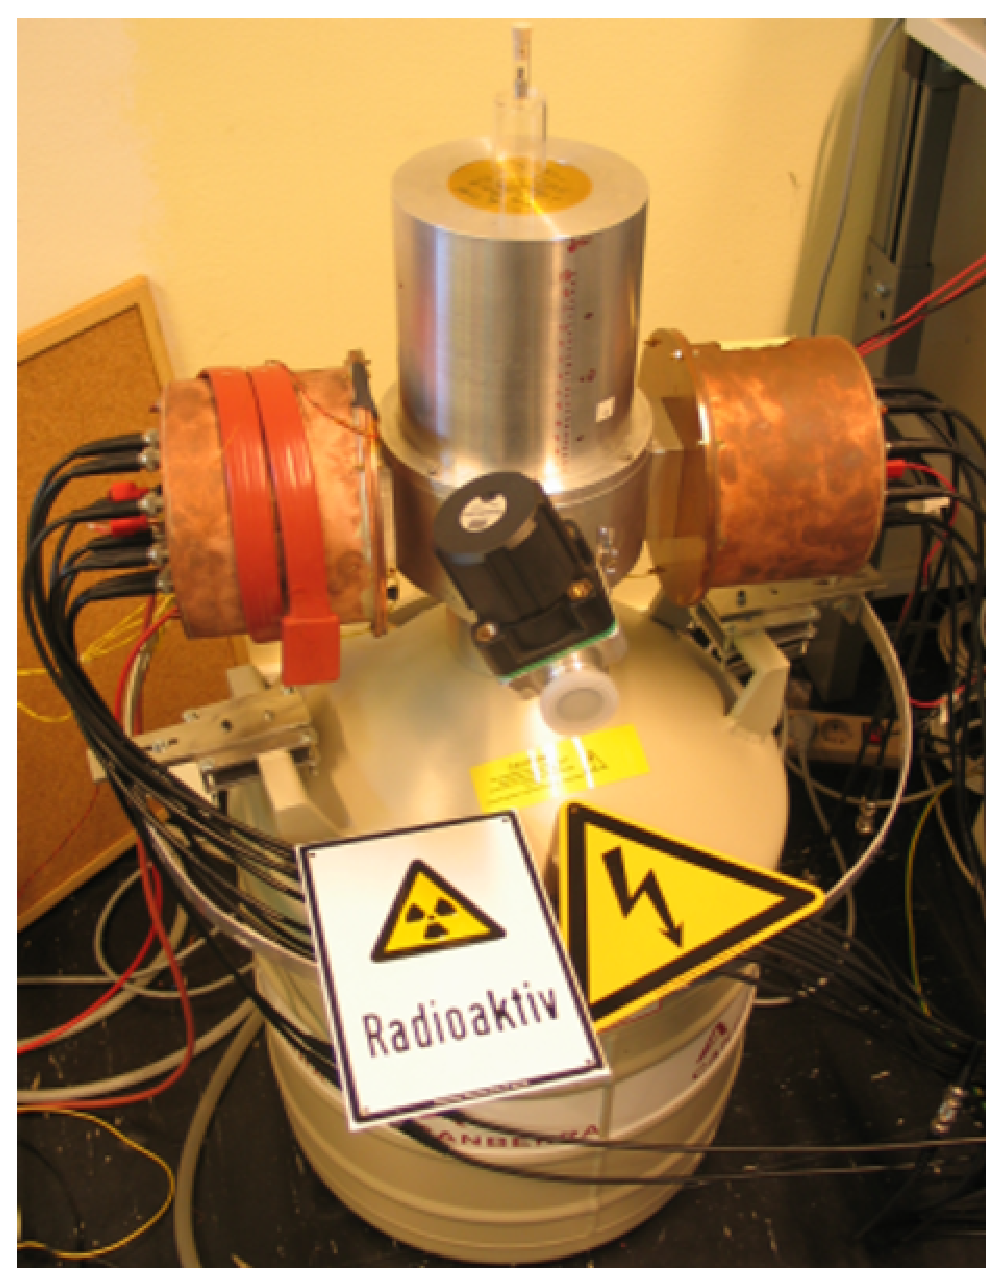
\includegraphics[height=0.25\textheight]{comcryo}}\hfil%
  \subfloat[Copper ears housing pre-amplifiers]{\label{fig:tt:ear}
    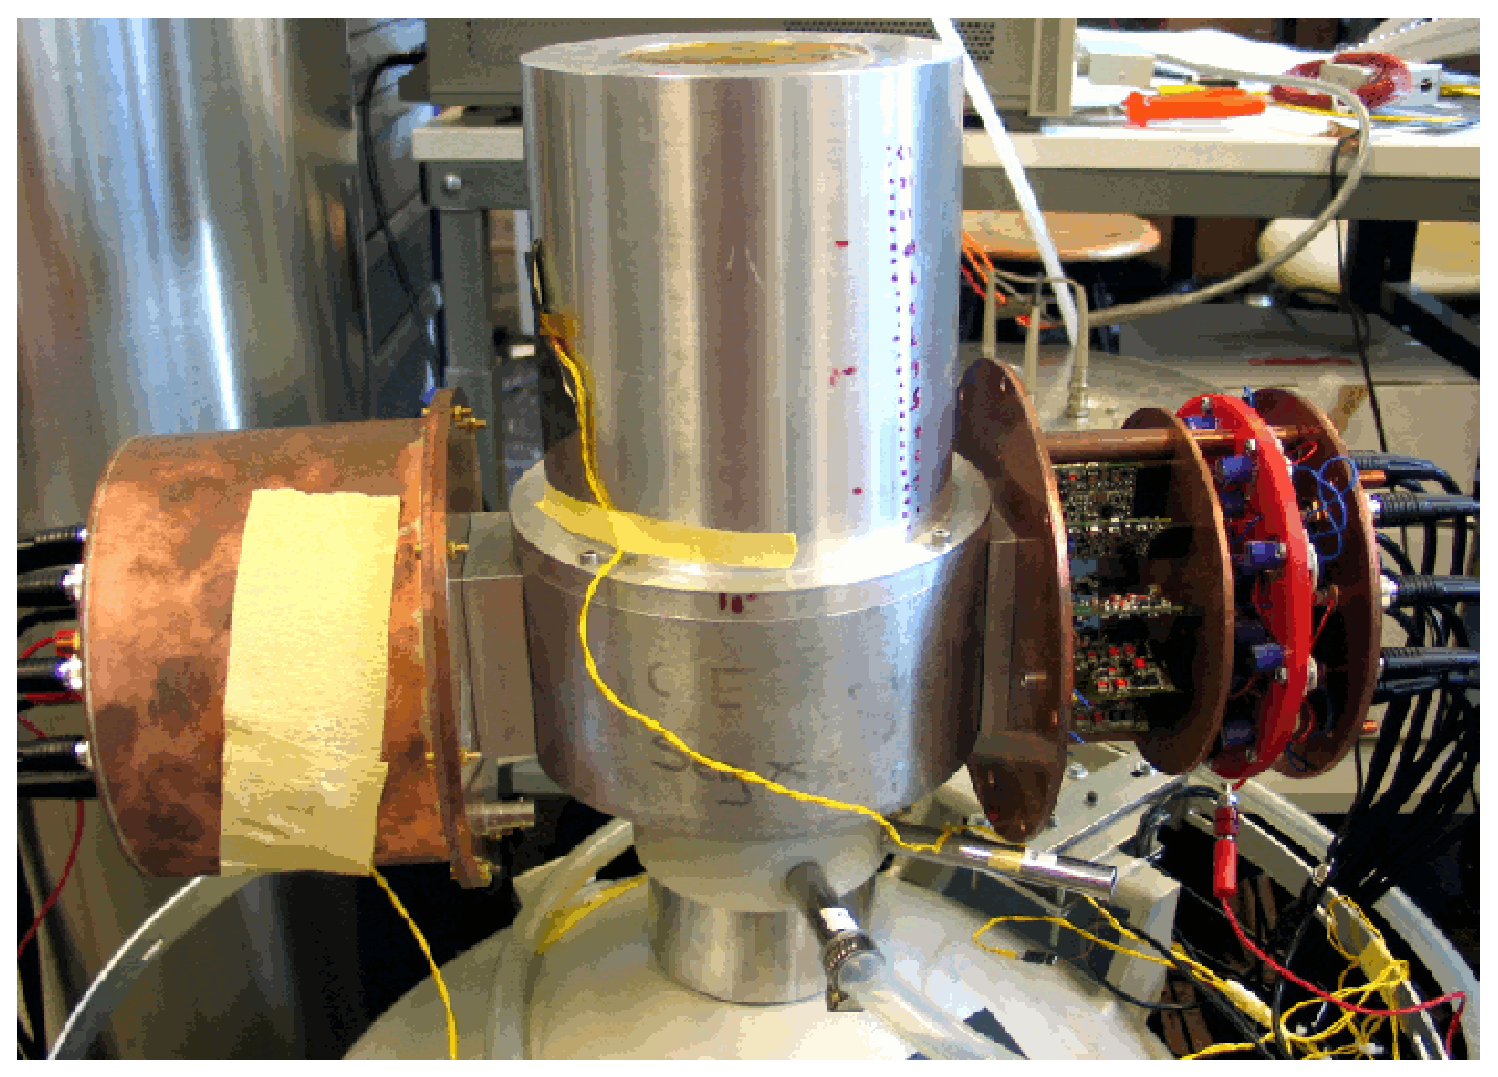
\includegraphics[height=0.25\textheight]{SIears}}%
  \caption{Test cryostat developed by Canberra-France: (a) the     standard liquid nitrogen dewar with the vacuum can on top and (b)     a close-up of the vacuum can and the copper ears housing the     pre-amplifier boards.}
  \label{fig:tt:comcryo}
\end{figure}

\subsection{Gerdalinchen II}
\label{sec:tt:gii}
Gerdalinchen II (GII in short) is a special cryostat developed by the technical division of Max-Planck-Institut f\"ur Physik to test the operation of up to three segmented germanium detectors submerged in cryogenic liquid. Fig.~\ref{fig:tt:g2} is a schematic of the main body of GII, a two-walled cryogenic dewar inside a cylindrical aluminum tank with a height of 960~mm and a diameter of 612~mm. The top flange can be removed upwards allowing the mounting of detectors to a vertical stainless steel bar under the flange, see Fig.~\ref{fig:tt:g2d}. Figure~\ref{fig:tt:g2n} shows the operation of a detector inside GII with a neutron source placed aside. 

\begin{figure}[tbhp]
  \centering
  \subfloat[Schematic of GII]{\label{fig:tt:g2}
    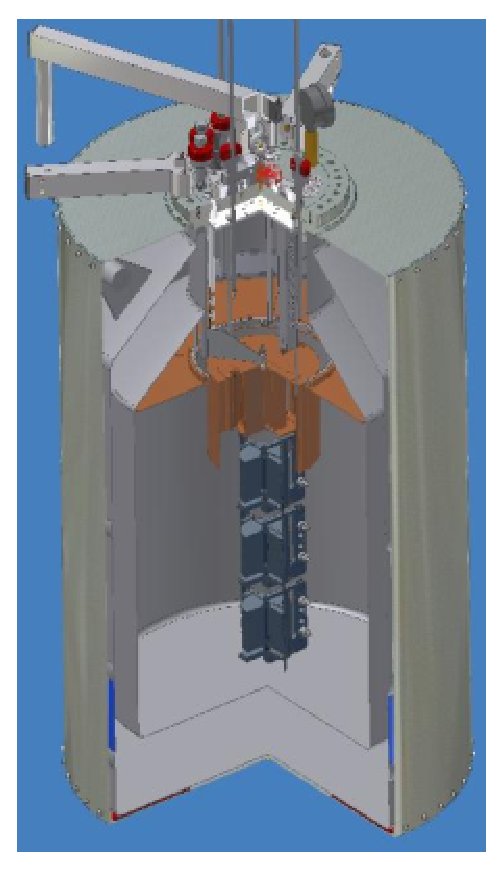
\includegraphics[height=0.25\textheight]{GIIdraw}}\hfil%
  \subfloat[GII in operation with a neutron source]{\label{fig:tt:g2n}
    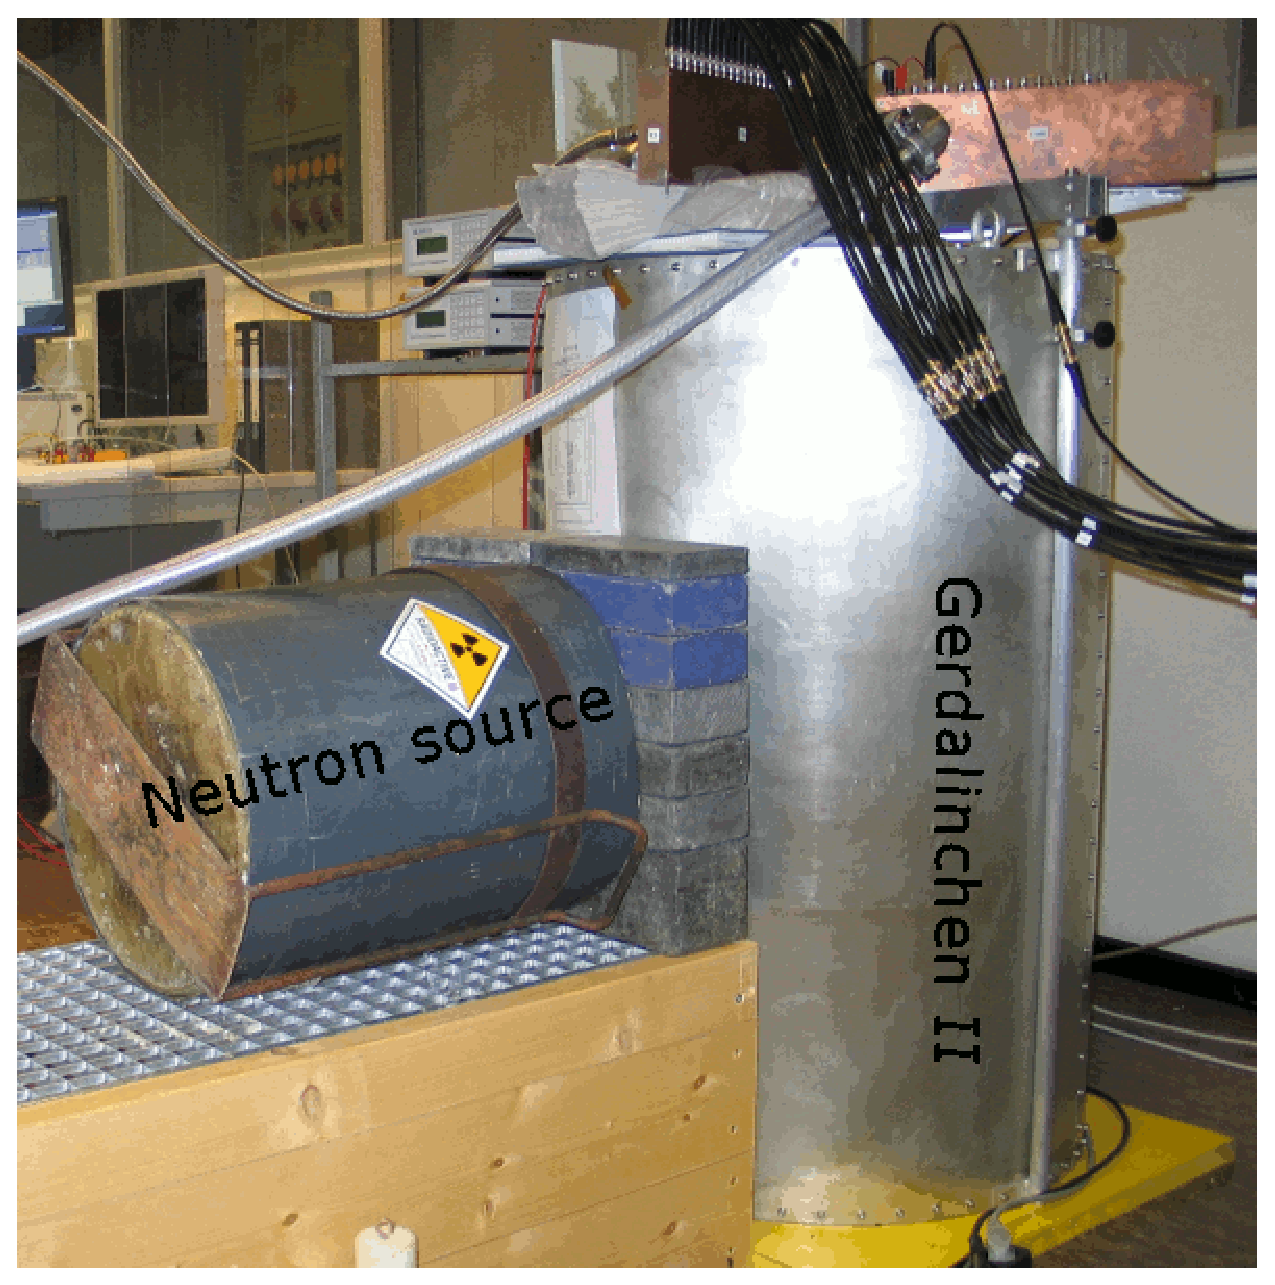
\includegraphics[height=0.25\textheight]{GIIneutron}}\hfil%
  \subfloat[Detector installation above GII dewar]{\label{fig:tt:g2d}
    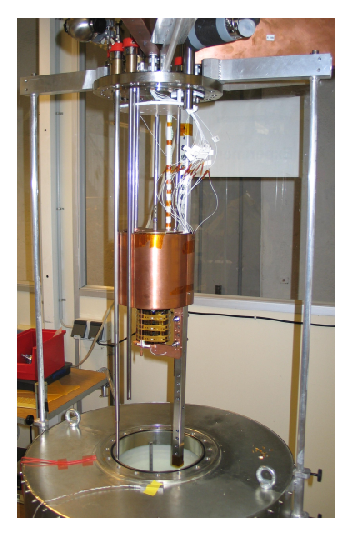
\includegraphics[height=0.25\textheight]{GIIdet}}%
  \caption{Gerdalinchen II cryostat.}
  \label{fig:tt:gii}
\end{figure}

There are three high voltage feed-throughs and four signal connectors, each with 18 channels, on the top flange. This allows the operation of three 18-fold segmented detectors simultaneously. The flange also facilitates the re-filling of the dewar with cryogenic liquid, the flushing with gaseous nitrogen and the evaluation of the dewar without opening the system. The dewar is re-filled daily to keep the level of cryogenic liquid above the infrared shields (see Fig.~\ref{fig:tt:g2}). The liquid level is monitored using several PT100 thermal resistances mounted at different places inside the dewar.


\section{Electronics} 
\label{sec:tt:ele} 

\subsection{Front-end}
\label{sec:tt:fend} 
An electronic diagram of a segmented detector mounted in the vacuum can and its read out scheme are shown in Fig.~\ref{fig:tt:sifa}. The signals were read out using charge sensitive PSC-823C pre-amplifiers[] with a decay time of 50~$\mu$s. The FET for the core electrode was mounted inside the cryostat close to the detector, the FETs for the segment electrodes were incorporated into the pre-amplifier boards which were housed inside the copper ears on both sides of the detector as shown in Fig.~\ref{fig:tt:ear}. Figure~\ref{fig:tt:sifb} depicts the layout of the feed-throughs between the vacuum can and the copper ears.

\begin{figure}[tbhp]
  \centering
  \subfloat[Read-out scheme of segmented detector mounted in the   vacuum can]{\label{fig:tt:sifa}
  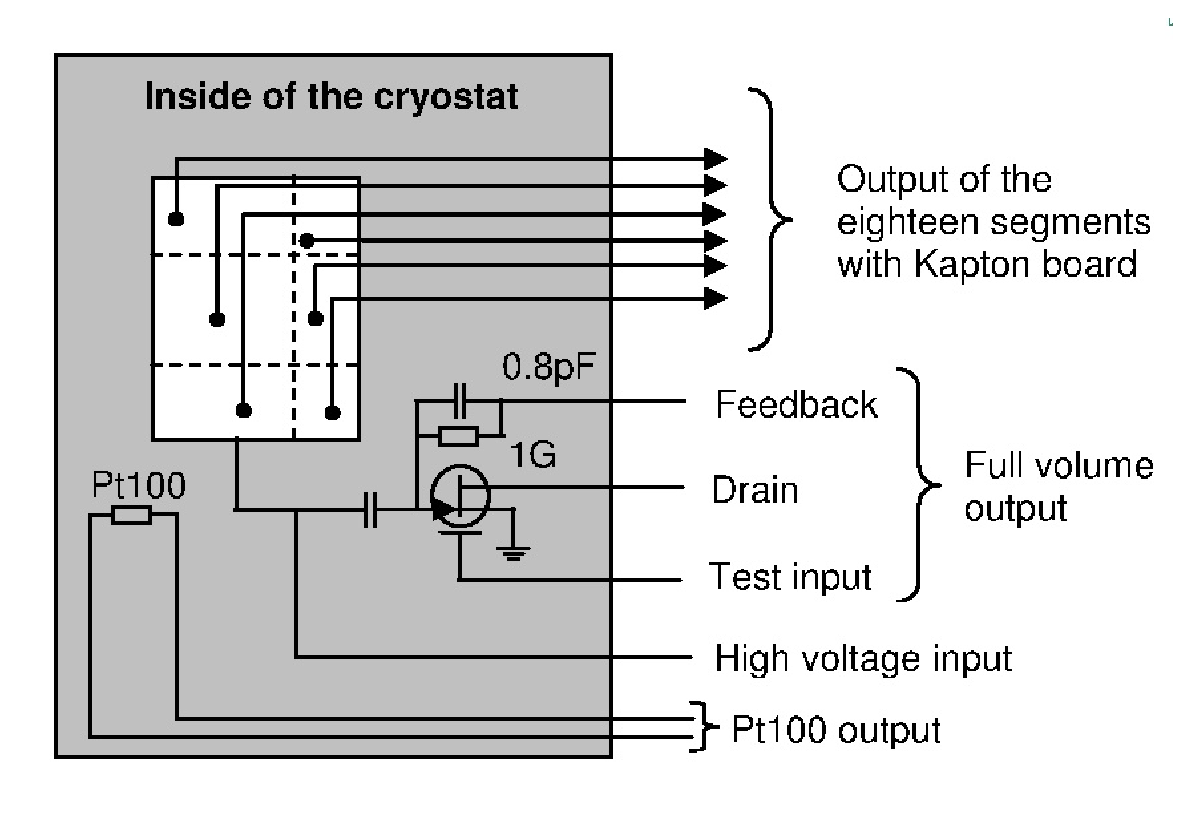
\includegraphics[height=0.25\textheight]{block1}}\hfil%
\subfloat[Layout of the feed-throughs between the vacuum can and the copper ears]{\label{fig:tt:sifb}
  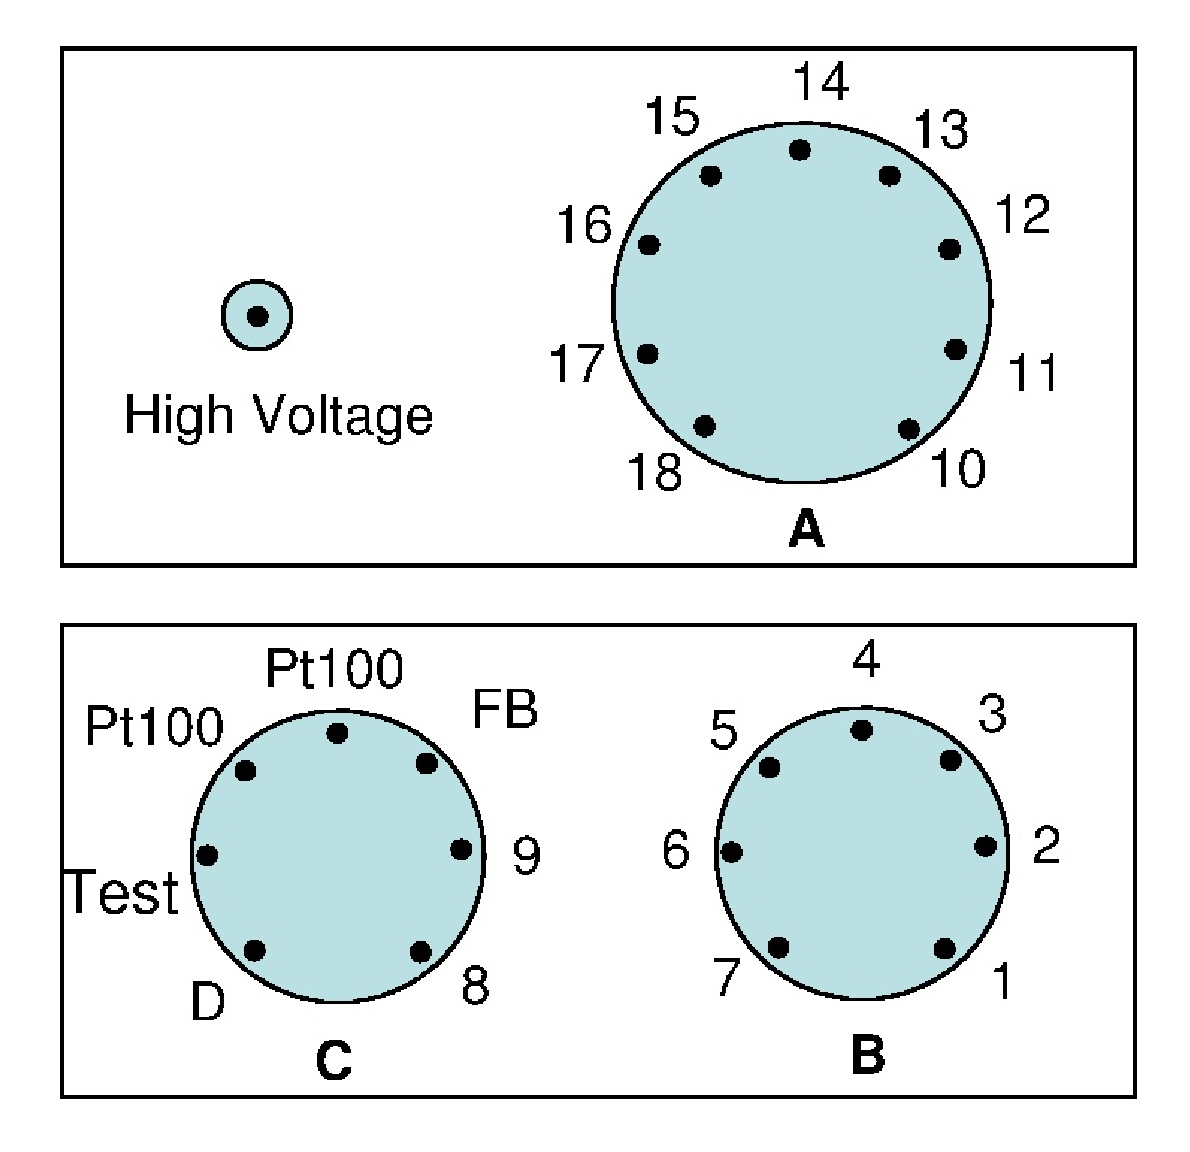
\includegraphics[height=0.25\textheight]{block2}}%
\caption{Frond-end electronics of a segmented detector mounted in the   vacuum can.}
  \label{fig:tt:sif}
\end{figure}

In GII a different setup was used. The FET for the core electrode was incorporated into the pre-amplifier boards like the segment electrodes. Thus, the cross talks from the core signal to the segment signals was minimized. All the pre-amplifier boards were mounted in a copper box and shared a common ground as shown in Fig.~\ref{fig:tt:gefb}. The filters for the high voltage lines and the coupling capacitors for the core signal cables were placed under the top flange as shown in Fig.~\ref{fig:tt:gefa}. They were first operated above the cryogenic liquid level and later submerged for better temperature stability.
\begin{figure}[tbhp]
  \centering
  \subfloat[High voltage filters and coupling capacitors in GII]{\label{fig:tt:gefa}
    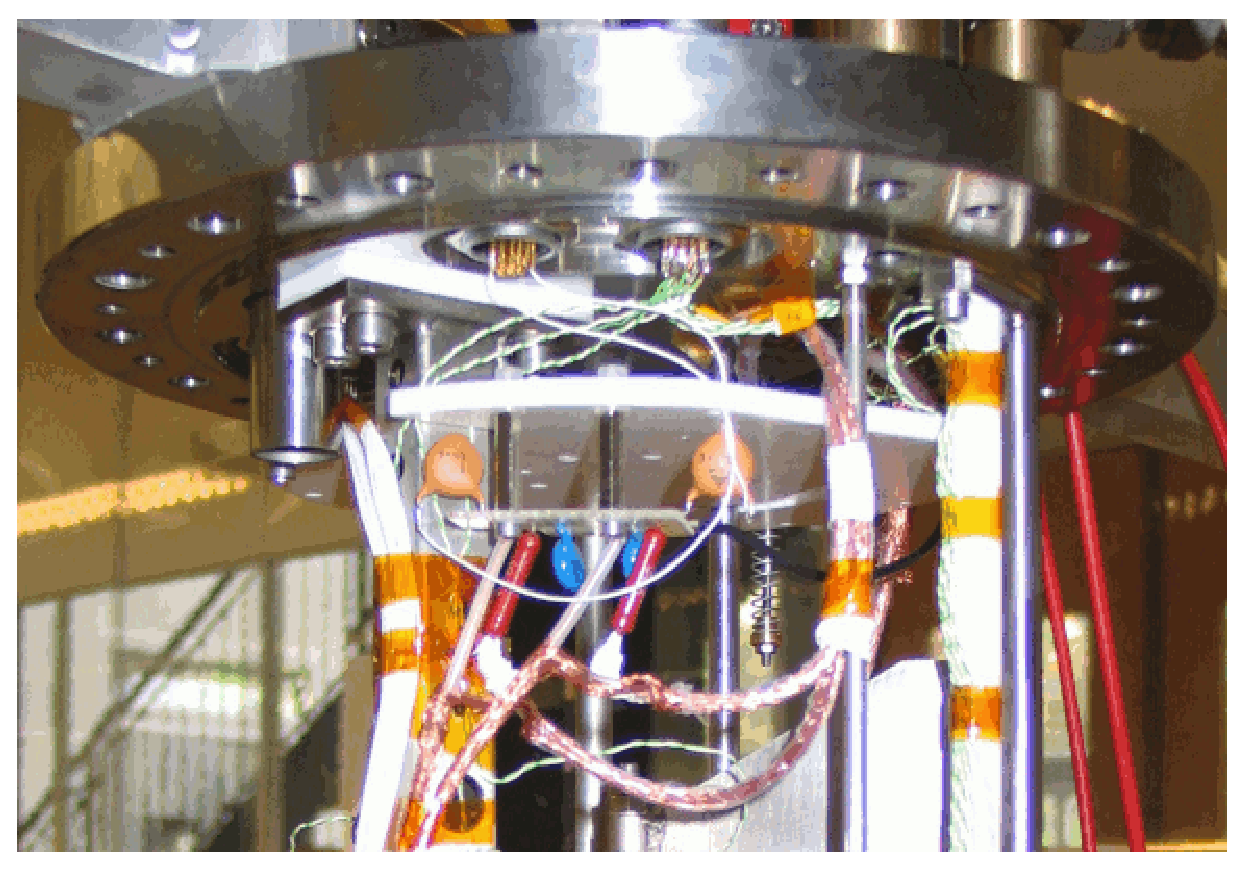
\includegraphics[height=0.2\textheight]{GIIHV}}\hfil%
  \subfloat[Pre-amplifier box for a segmented detector in GII]{\label{fig:tt:gefb}
  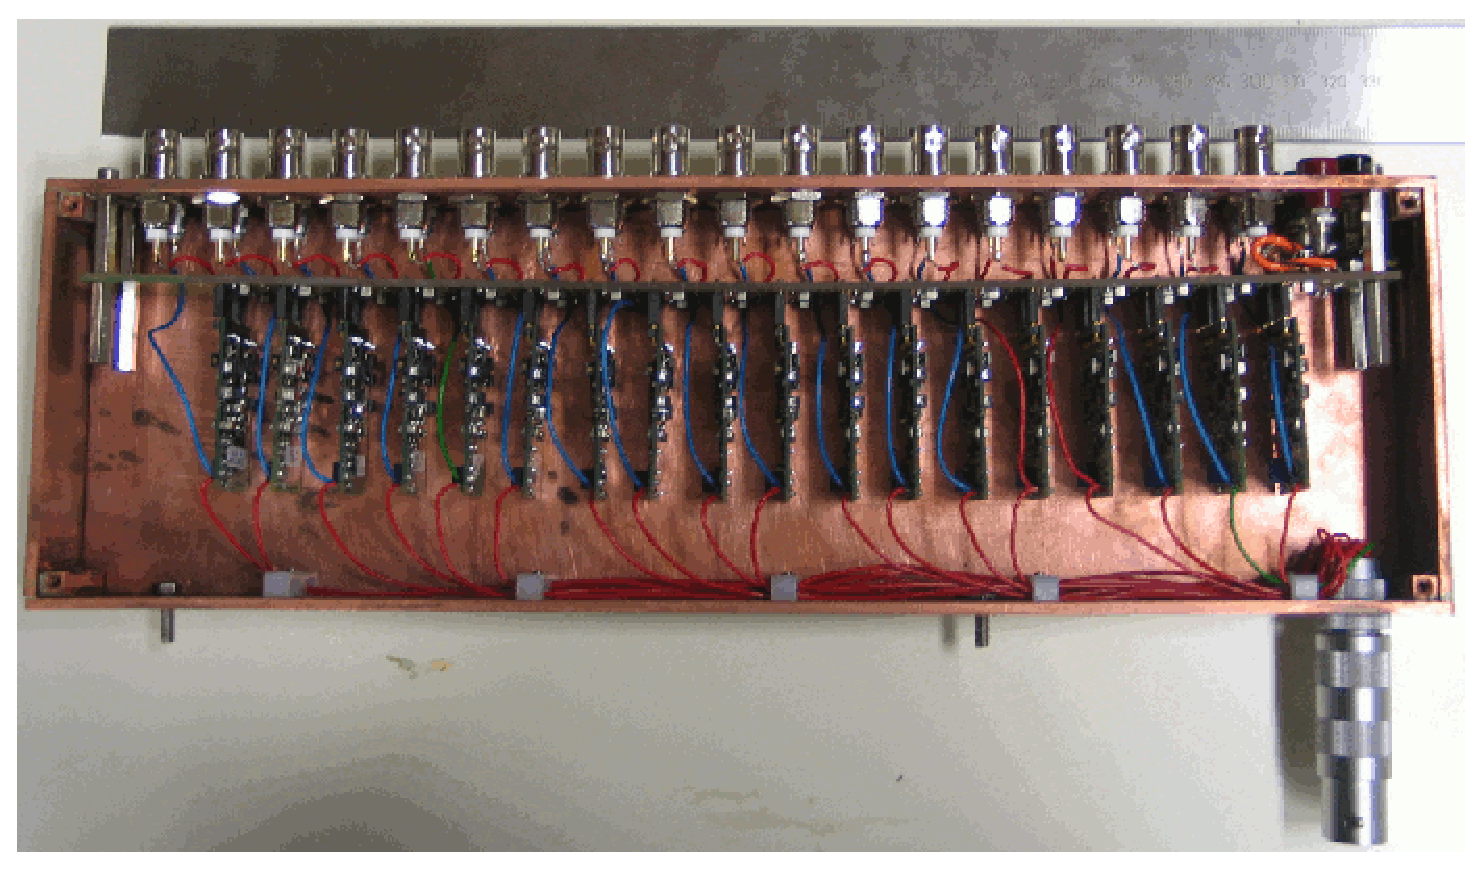
\includegraphics[height=0.2\textheight]{GIIpreamp}}%
  \caption{Front-end electronics in GII.}
  \label{fig:tt:gef}
\end{figure}

\subsection{DAQ} 
\label{sec:tt:daq}
The pre-amplified signals are digitized using an XIA data acquisition system based on 14-bit ADC PIXIE-4 modules[] with a sampling rate of 75~MHz. The bandwidth of the analog signals is limited by a Nyquist filter to half the sampling rate, \textit{i.e.} 37.5~MHz. This avoids aliasing the noise from higher frequencies. It is implemented in the analog section of the PIXIE-4 module as a low-pass Sallen-Key filter that makes a sharp (but finite) cut-off at this frequency. Energies are calculated using software filters~\cite{Pixie4}. Recorded pulse shape data consist of 300 samples of the integrated charge amplitude. The onset of the signal can be set by hand and was set to 1~$\mu$s for most of the measurements. The trigger and energy thresholds of the core and segment electrodes can be set to different values. Pile-up pulses can be rejected or stored using a rough energy estimation.


\section{Monitoring} 
\label{sec:tt:lamo}
The operation of the test facilities requires the monitoring of high voltage supplies, temperature monitors, vacuum gauges, oxygen sensors, etc. The monitoring needs to be automated for overnight or long term measurements. A generalized ``Laboratory Monitor system'', LaMo, was developed to monitor and control most of the hardware in the laboratories using the graphic programming language, LabVIEW[]. The system has a set of user friendly interfaces to perform most of the common lab tasks and a modularized design of the functionalities to facilitate the implementation of new pieces of hardware.

Fig.~\ref{fig:tt:lamo} shows the control panels of LaMo. The main panel is called ``Laboratory'' as shown in Fig.~\ref{fig:tt:plab}. It shows a list of experiments going on in the laboratory and their status. An experiment can be created, edited, started, stopped using the buttons next to the experiment list. The ``Laboratory'' panel also provides functions common to all experiments, such as email alerts, electricity, oxygen sensors, etc. Pieces of hardware to be associated to an experiment can be chosen from a list of available hardware. This is done in the ``Config'' panel of LaMo as shown in Fig.~\ref{fig:tt:pcon}, where pieces of hardware can be added, deleted from the list to be monitored. Once an experiment is created and configured, it is started from the ``Laboratory'' panel. An ``Experiment'' panel, as shown in Fig.~\ref{fig:tt:pexp}, where monitored variables are shown in different ways, automatically pop up. The functions specified for a particular experiment can be executed from there.

\begin{figure}[tbhp]
  \centering
  \subfloat[``Laboratory'' panel]{\label{fig:tt:plab}
    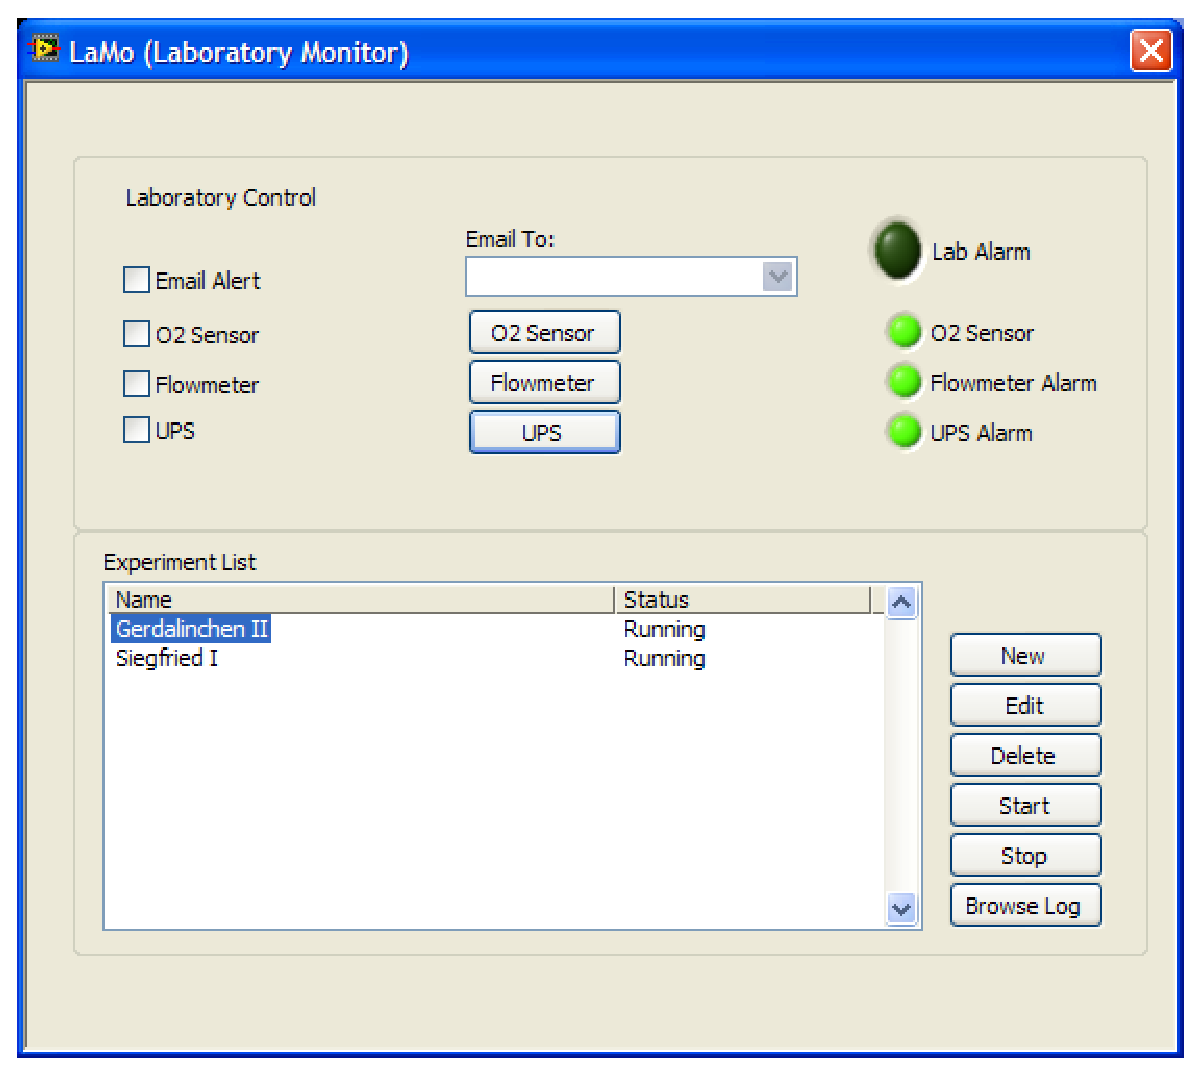
\includegraphics[height=0.23\textheight]{LaMoLab}}\hfil%
  \subfloat[``Config'' panel]{\label{fig:tt:pcon}
  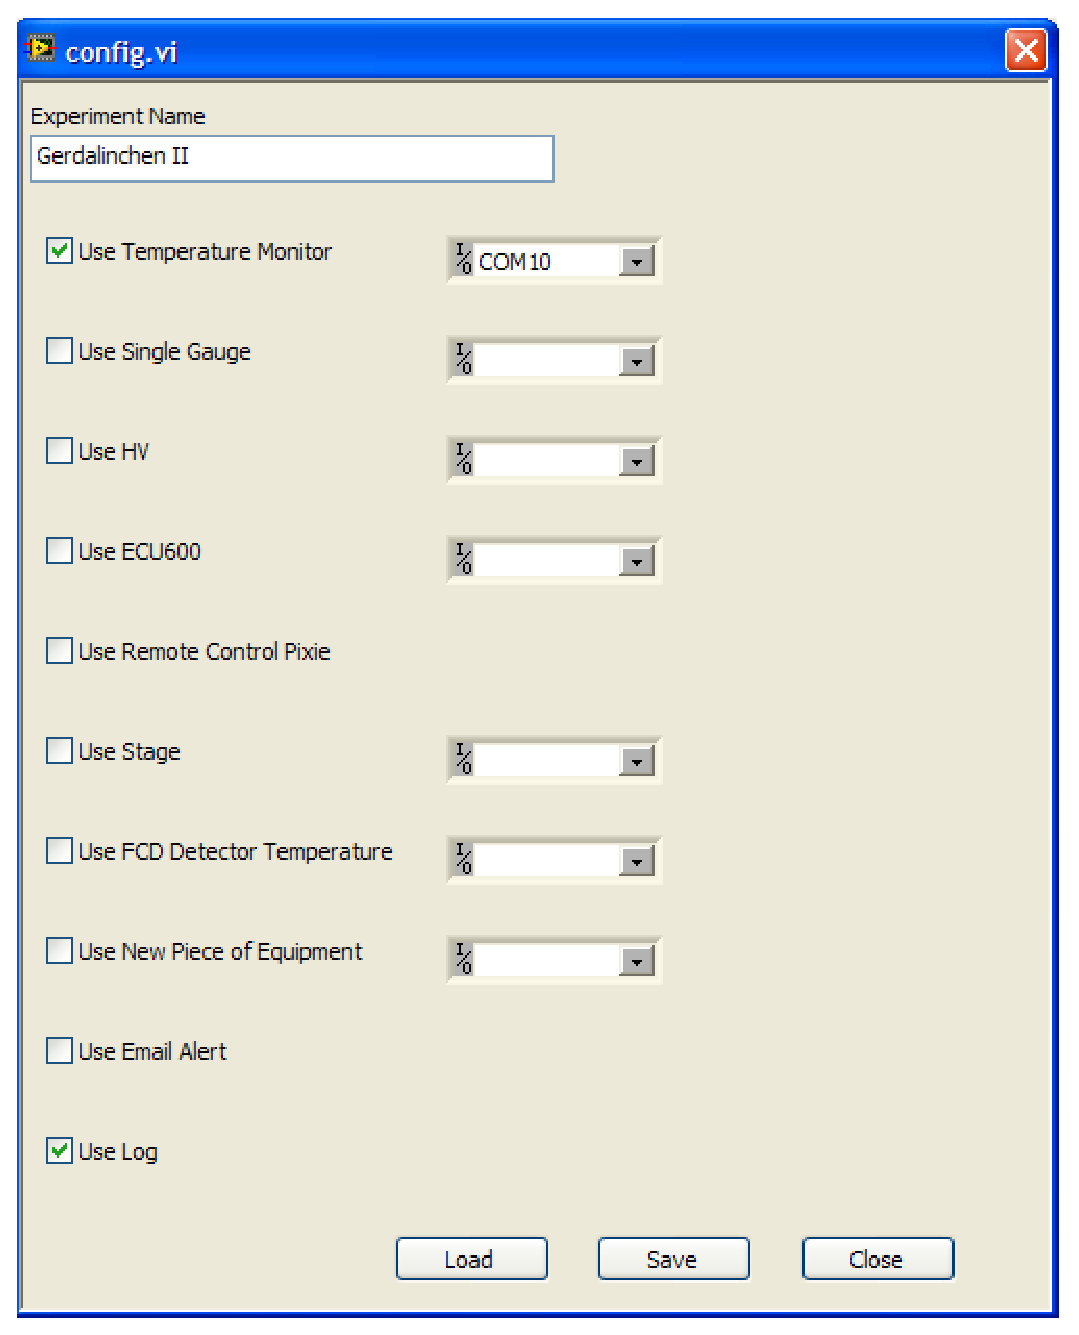
\includegraphics[height=0.23\textheight]{LaMoEdit}}\hfil%
  \subfloat[``Experiment'' panel]{\label{fig:tt:pexp}
  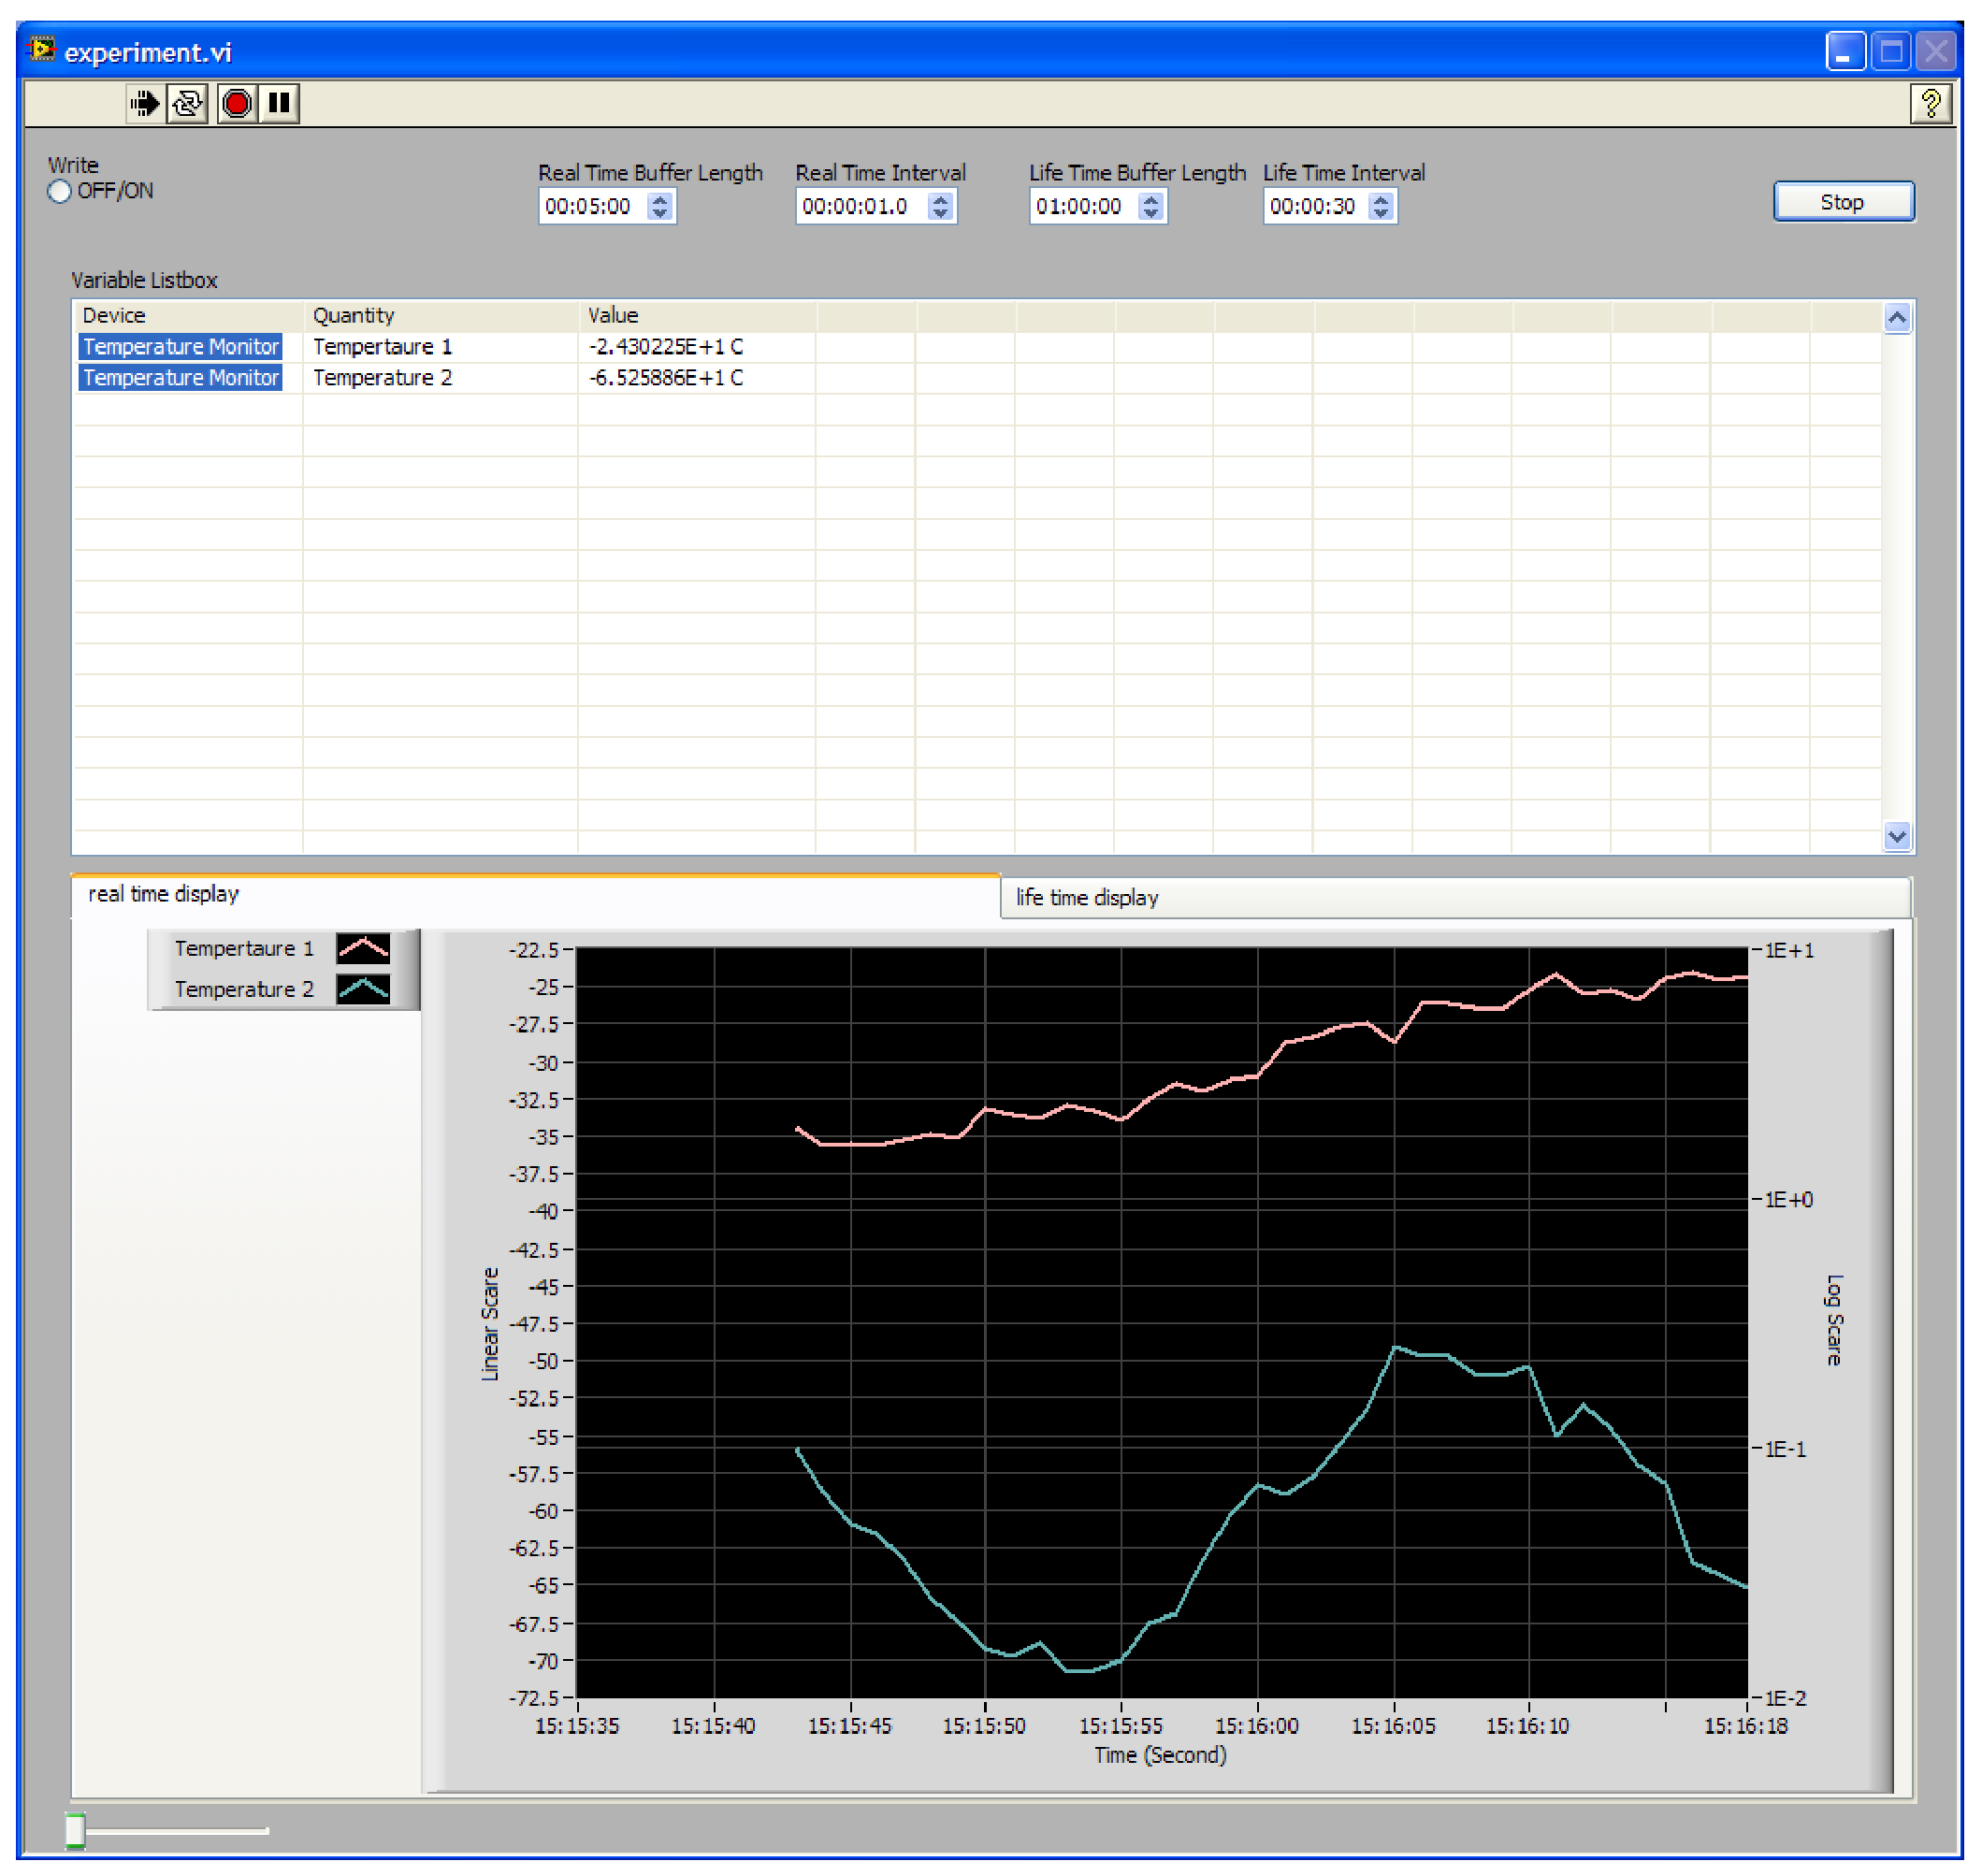
\includegraphics[height=0.23\textheight]{LaMoExp}}%
  \caption{Main panels of LaMo: (a) ``Laboratory'' panel: it provides a list of experiments and their status, and gives access to functions common to all experiments; (b) ``Config'' panel: pieces of hardware to be associated to an experiment can be added, deleted from the list to be monitored; (c) ``Experiment'' panel: various displays of monitored variables can be requested and the execution of experimental tasks can be steered.}
  \label{fig:tt:lamo}
\end{figure}

The common user interface enforces common I/Os for different pieces of hardware. The functionality of LaMo is modularized so that the effort to implement a new piece of hardware is minimized. To add a new piece of equipment the developer only needs to define its I/O interface to LaMo. The other efforts, such as programming the user interface, etc., do not have to be repeated every time.


%%% Local Variables:
%%% mode:latex
%%% TeX-master: "thesis"
%%% End:

\clearpage{\pagestyle{empty}\cleardoublepage}

\chapter{Gerdalinchen II}
\label{cha:gerdalinchenII}
\chapter[Operation of segmented detectors in LN$_{2}$]{Operation of segmented detectors in liquid nitrogen}
\label{cha:GII}
Segmented n-type germanium detectors will be directly submerged in cryogenic liquid in GERDA Phase II. It is therefore very important to study the performance of segmented detectors in cryogenic liquid. Siegfried II, the second 18-fold segmented n-type prototype detector for GERDA Phase II (see Sec.\ref{sec:gerda:stat3}) was inserted into the Gerdanlinchen II test stand (see Sec.\ref{sec:tt:gii}) containing liquid nitrogen on April 23rd, 2008. It was kept in liquid nitrogen for about 5 months and was warmed up on September 15th, 2008. The resolution and leakage current of the core and all segments were constantly monitored. Four short cooling-down and warming-up cycles were carried out afterward to optimize the setup or to do some dedicated measurements. The leakage currents were monitored after each cooling-down. The results on the detector performance are summarized in this chapter.

\section{Experimental setup}
\label{sec:gii:setup}
The measurements were performed using the cryogenic test stand, Gerdalinchen II (GII in short). The detailed description of GII can be found in Sec.\ref{sec:tt:gii}.  Figure~\ref{fig:ii:sch} shows the setup of GII for the operation of segmented detectors in liquid nitrogen. Liquid nitrogen was filled into the dewar through the cryogenic liquid filling tube. The numbers inside the parentheses indicate the positions of eight PT100 thermal resistors. They were used to monitor the level of the liquid nitrogen. The dewar was refilled per day to keep the level of liquid nitrogen between the second and the third PT100s. The infrared shields hence were kept inside liquid nitrogen ensuring the stability of the detector working temperature. There are three mounting positions for the detectors. Only the upper and middle ones were used in the measurements.

\begin{figure}[hbtp]
\centering
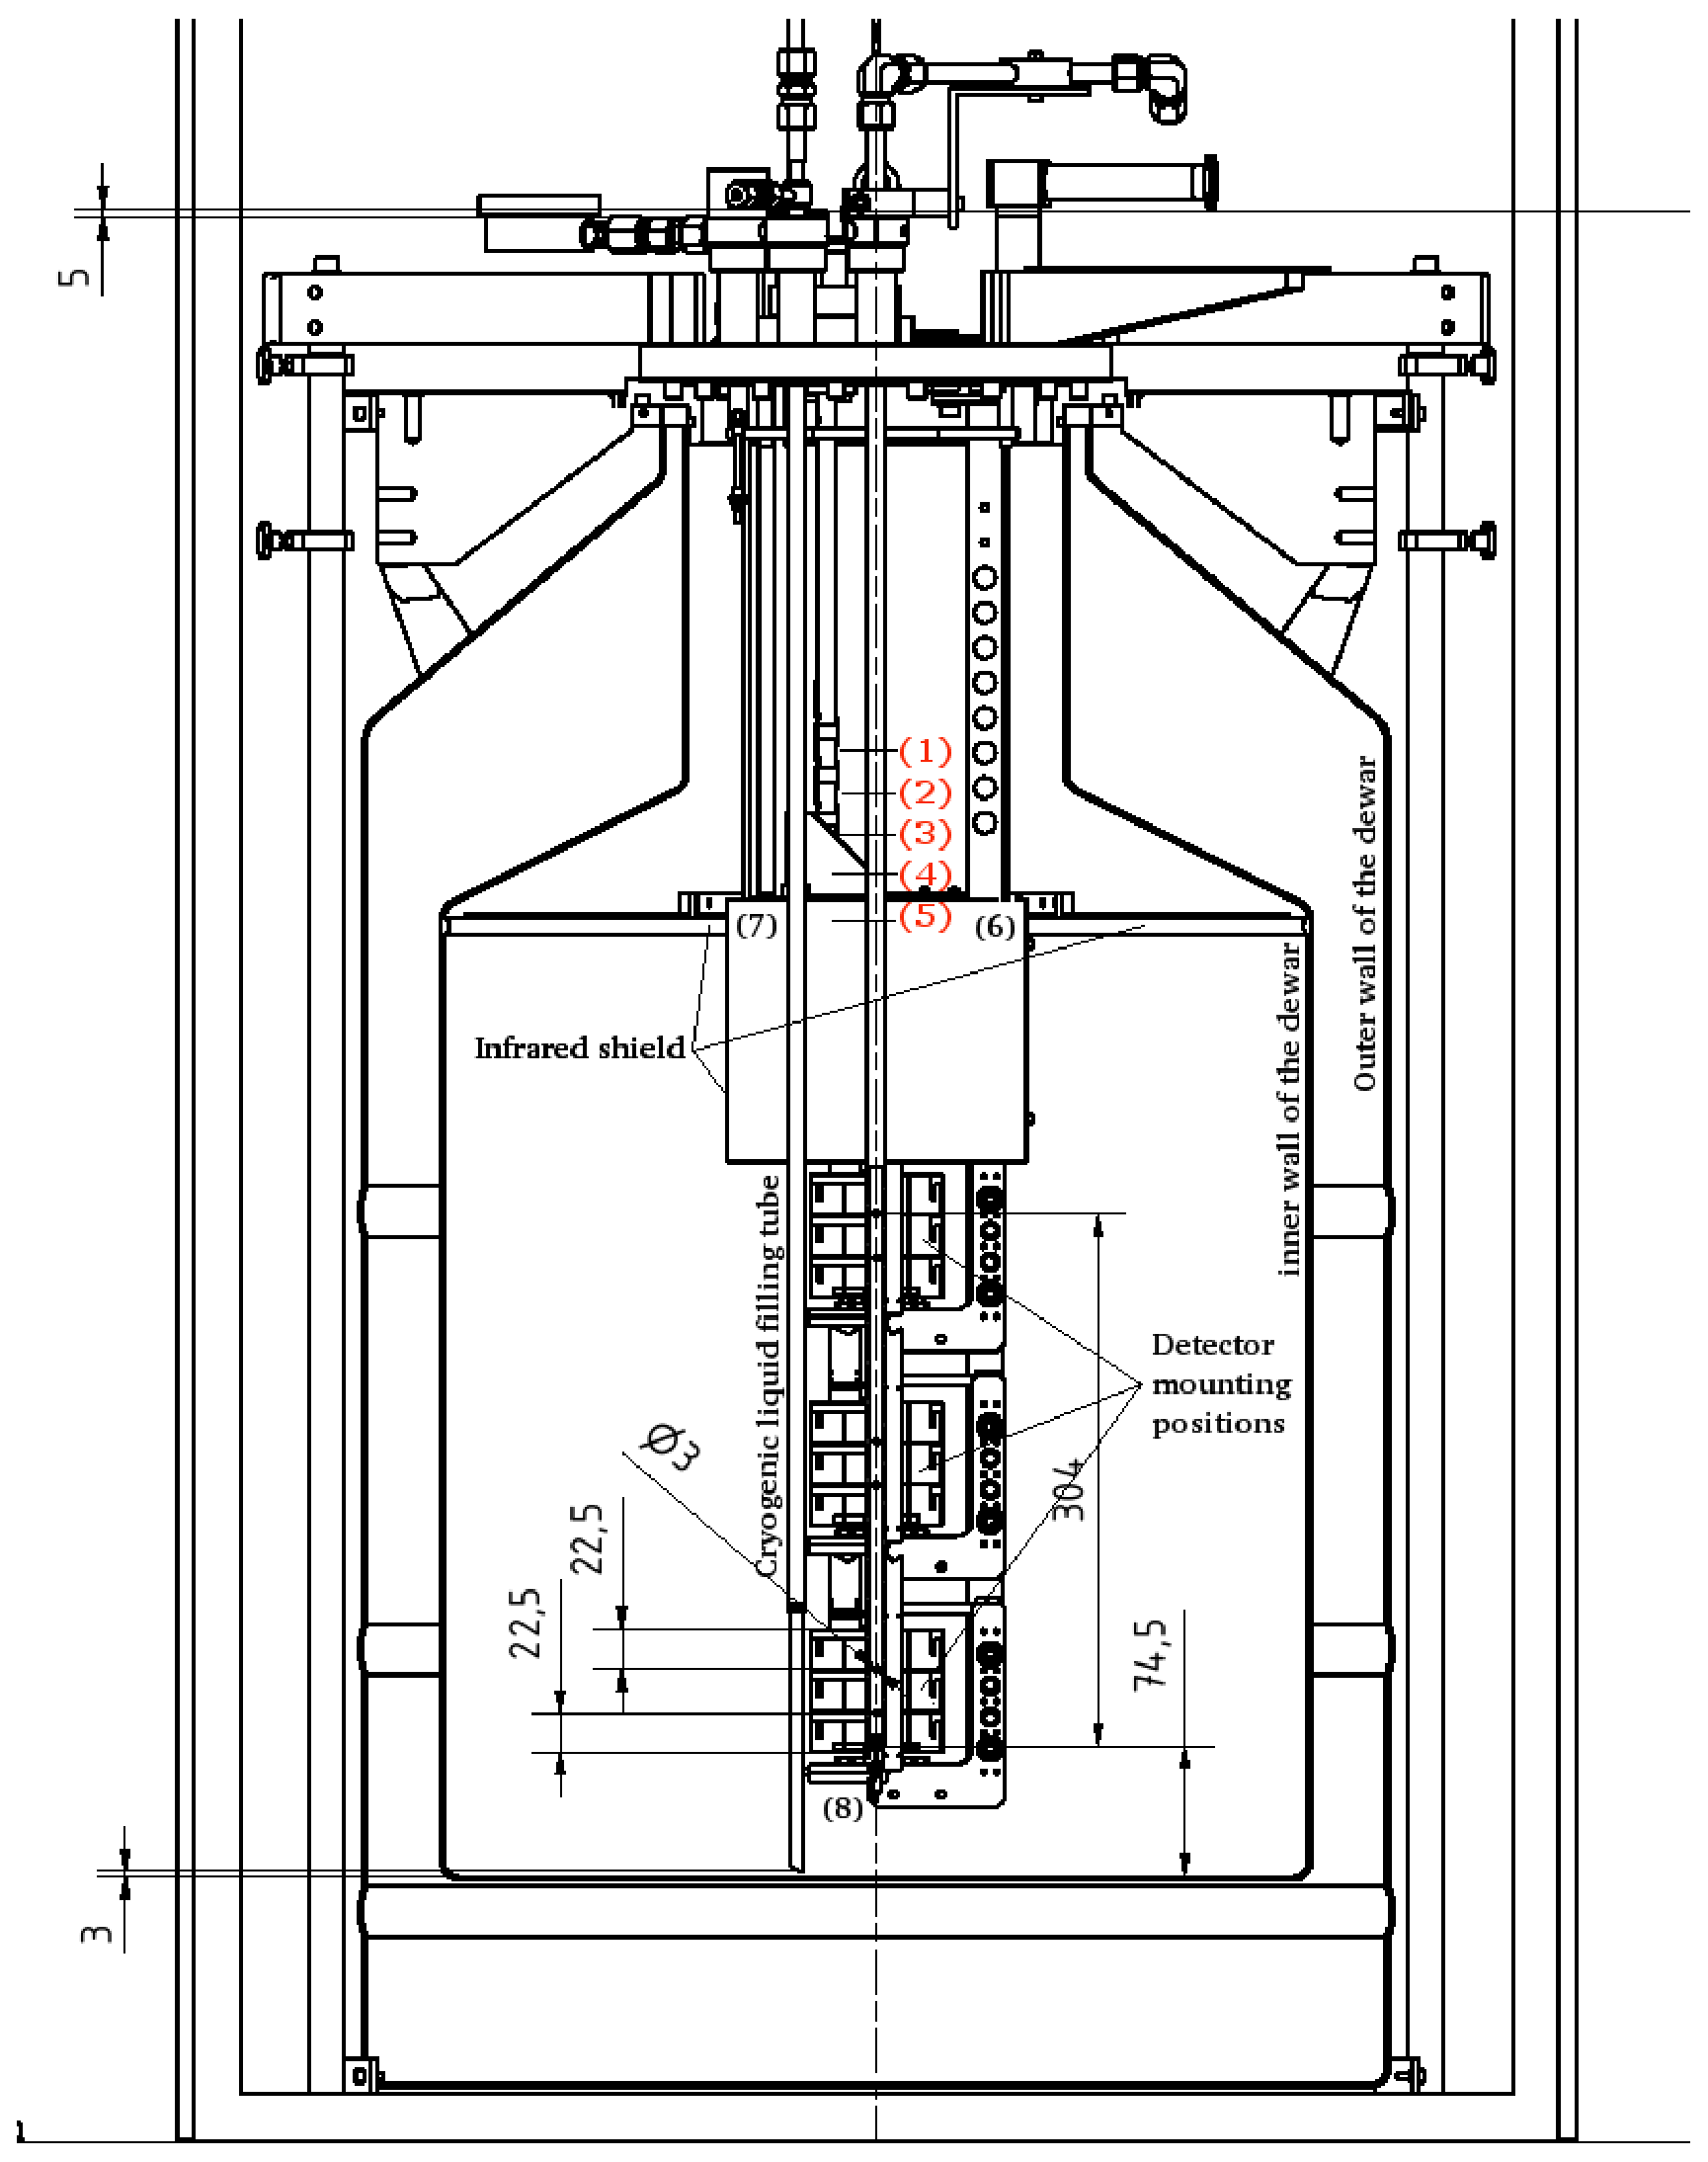
\includegraphics[width=\textwidth]{GIIscheme}
\caption{Gerdalinchen II setup for the operation of segmented detectors in liquid nitrogen.}
\label{fig:ii:sch}
\end{figure}

\section{Cooling test}
\label{sec:ii:cool}
The detector strings should be lowered into liquid argon at a moderate speed in GERDA so that the whole process can be finished in a reasonable time while the strings are kept in a stable situation. The designed submerging speed in GERDA is 10~mm/min. The temperature change of the detector during the submerging process was tested in GII with an aluminum mockup detector mounted in the highest position as shown in Fig.~\ref{fig:ii:sch}. The filling speed of liquid nitrogen was tuned to be about 10~mm/min. The tempareture profile of the mockup detector was monitored using three PT100 thermal resisters mounted on the top, bottom and in the middle of the mockup. Figure~\ref{fig:ii:temp} shows the tempareture changes of the mockup detector during the filling of GII. The positions of the 1$^{\text{st}}$ and the 8$^{\text{th}}$ thermal sensor are indicated in Fig.~\ref{fig:ii:sch}. Curves labled ``Top'', ``Middle'' and ``Bottom'' show the tempareture changes of the mockup detector. The largest tempareture difference between the top and bottom of the mockup detector is about 130~$^{\circ}$C. However, this large difference only lasted about 3 minutes. In most of the time the tempareture difference was very small.
\begin{figure}[htbp]
\centering
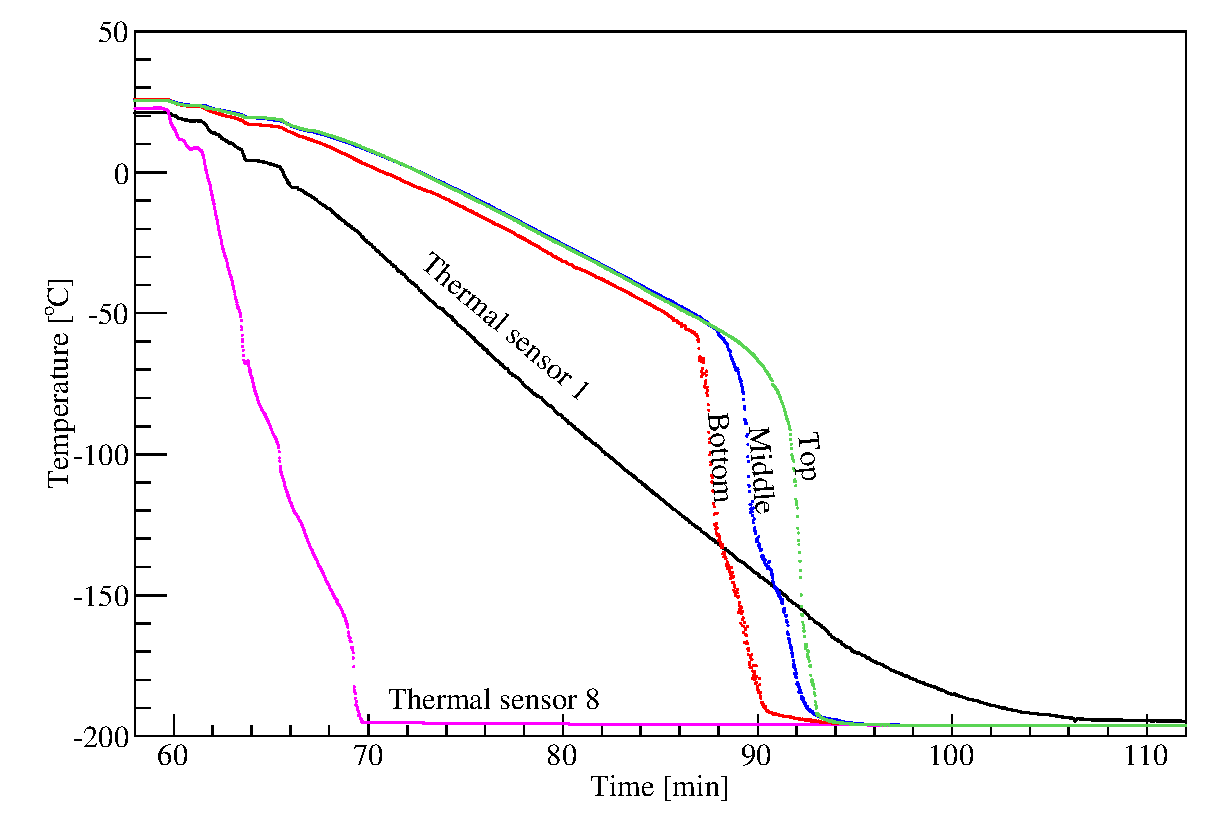
\includegraphics[width=0.8\textwidth]{temp}
\caption{Temperature profile of mockup detector during cooling down process. GII was filled with liquid nitrogen at the speed of 10~mm/min. Positions of the 1$^{\text{st}}$ and the 8$^{\text{th}}$ thermal sensor are indicated in Fig.~\ref{fig:ii:sch}. Curves labled ``Top'', ``Middle'' and ``Bottom'' show the tempareture changes of the mockup detector.}
\label{fig:ii:temp}
\end{figure}

\section{History of resolution}
\label{sec:ii:sigma}
Siegfried II was mounted at the hightest detector mounting position in GII after a detailed cooling procedure was worked out. It was cooled down on April 23$^{\text{rd}}$, 2008. The core and segment resolutions of Siegfried II were constantly monitored during the 140 days of operation. The variation of the resolution (FWHM) at 1332~keV is shown for the core channel in Fig.~\ref{fig:ii:fwhm_core} and for all 18 segments in Fig.~\ref{fig:ii:fwhm_segs}.
\begin{figure}[hbtp]
\centering
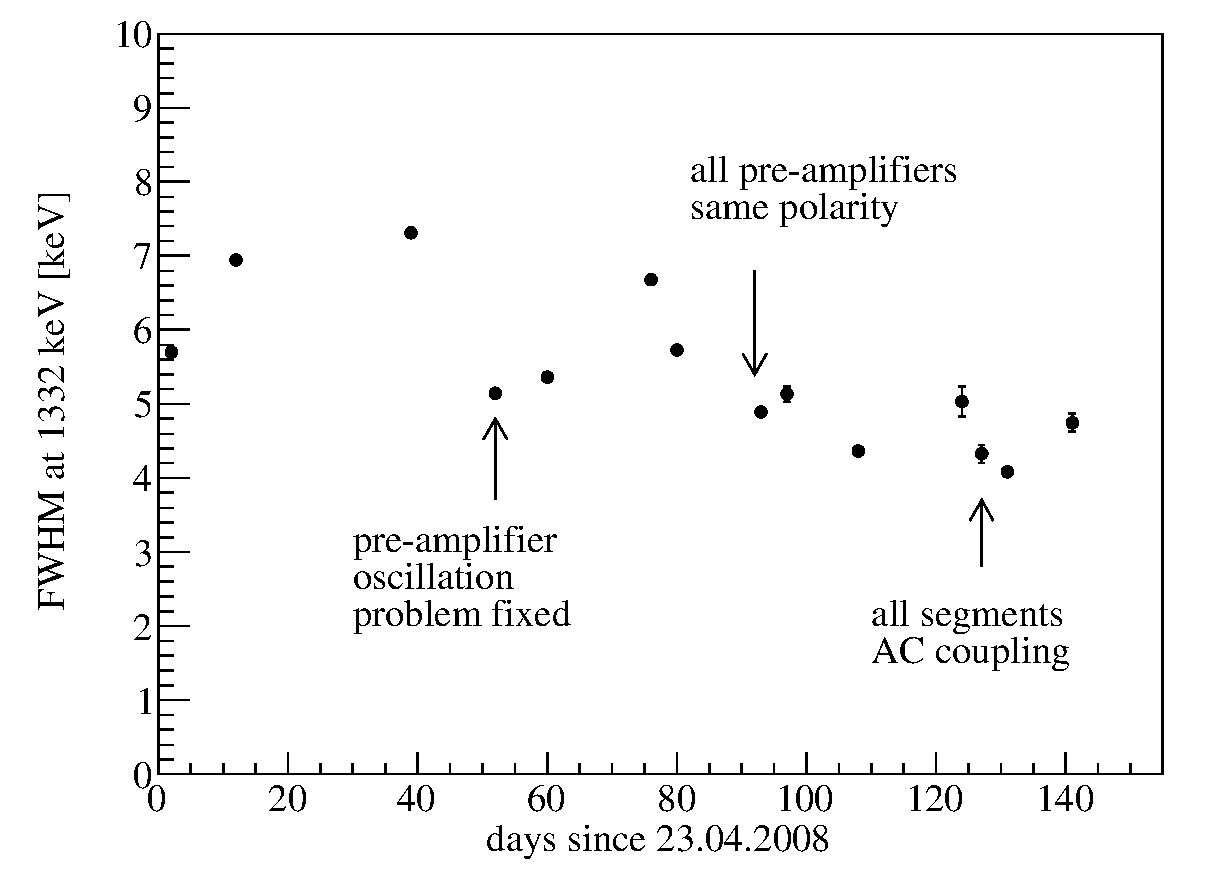
\includegraphics[width=0.6\textwidth]{fwhm_versus_time_core}
\caption{History of the core resolution of Siegfried II during 140 days of operation.}
\label{fig:ii:fwhm_core}
\end{figure}

\begin{sidewaysfigure}[tphb]
\centering
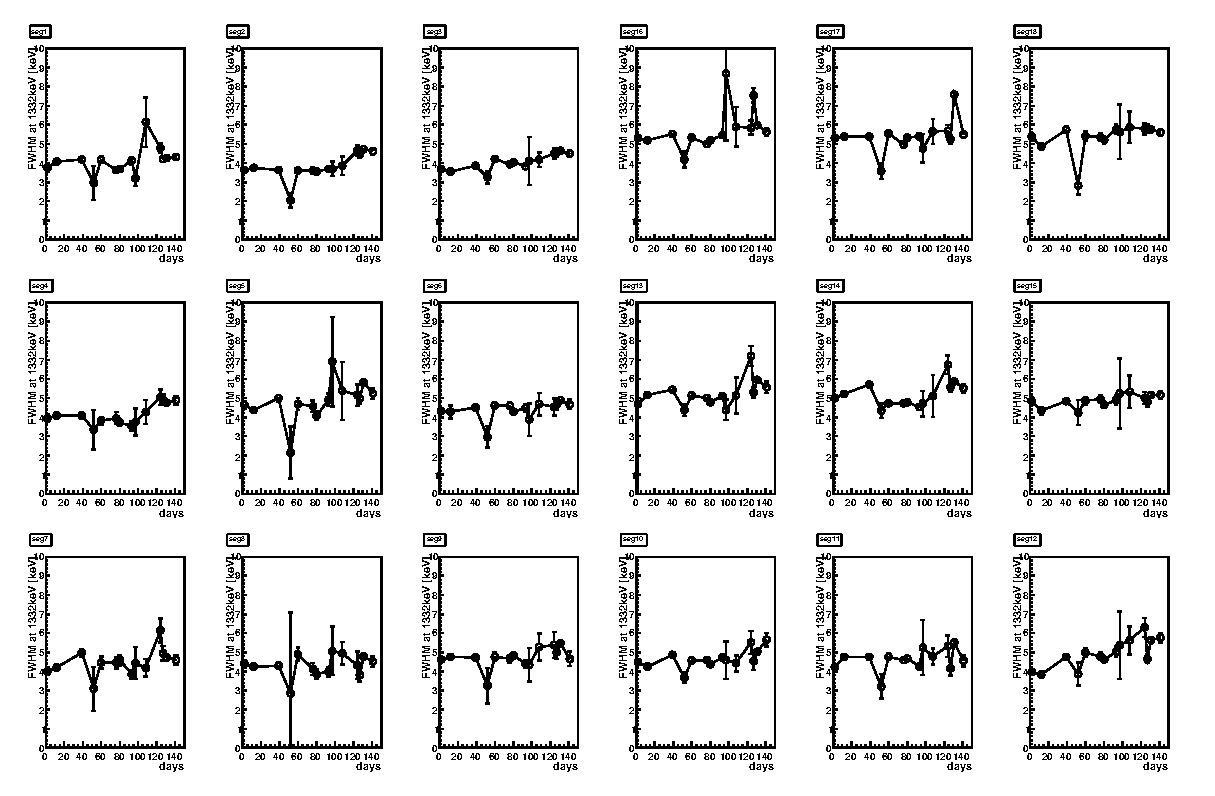
\includegraphics{fwhm_versus_time_segments}
\caption{History of the segment resolutions of Siegfried II during 140 days of operation.}
\label{fig:ii:fwhm_segs}
\end{sidewaysfigure}

During the first month of operation, all preamplifiers were oscillating if all 19 channels were read out simultaneously. The oscillation was due to the bad grounding scheme of the copper boxes holding and shielding the preamplifiers (see Fig.~\ref{fig:tt:gefb}). The problem was fixed by adding an extra copper plate inside the box, which serves as the commond ground for all preamplifiers. Afterwards, all preamps could be read out simultaneously
and the core resolution was slightly improved as well.

The second problem which affected the core resolution was related to the pulse polarity of the preamplifiers. Three preamplifiers (segments 3, 15 and 17) had negative signal pulse while the rest had positive pulse. Though the polarity of these three preamplifiers were corrected in the DAQ system, certain cross talks were observed between these three preamplifiers and the core preamplifier. Take the 1332~keV photon line as an example, for events with the photon energy deposited inside any of these three segments the energy measured by the core preamplifer is about 2~keV smaller than the measured core energy in those events with the same photon energy deposited inside any other segments. These three preamplifiers were then replaced, resulting in some improvement in the core resolution as indicated in Fig.~\ref{fig:ii:fwhm_core}.

In order to obtain a better defined potential of segments, all segment preamplifiers were modified from DC to AC coupling ten days before the first warming up, using 1~G$\Omega$ resistors and 2.2~nF capacitors. This improved slightly the core resolution, but not those of the segments.


\section{Leakage current}
\label{sec:ii:current}
The leakage current of Siegfried II at 2000~V was constantly monitored during the first 140 days of operation. Two measurement methods were used: (a) direct measurement with a peco-amparemeter and (b) indirect measurement by comparing the baseline movement at 0~V and 2000~V. The results from these two different measurements are both shown in Fig.~\ref{fig:ii:lc}. The leakage current stayed constantly around 20~pA except one measurement which was probably performed incorrectly.

\begin{figure}[htbp]
\centering
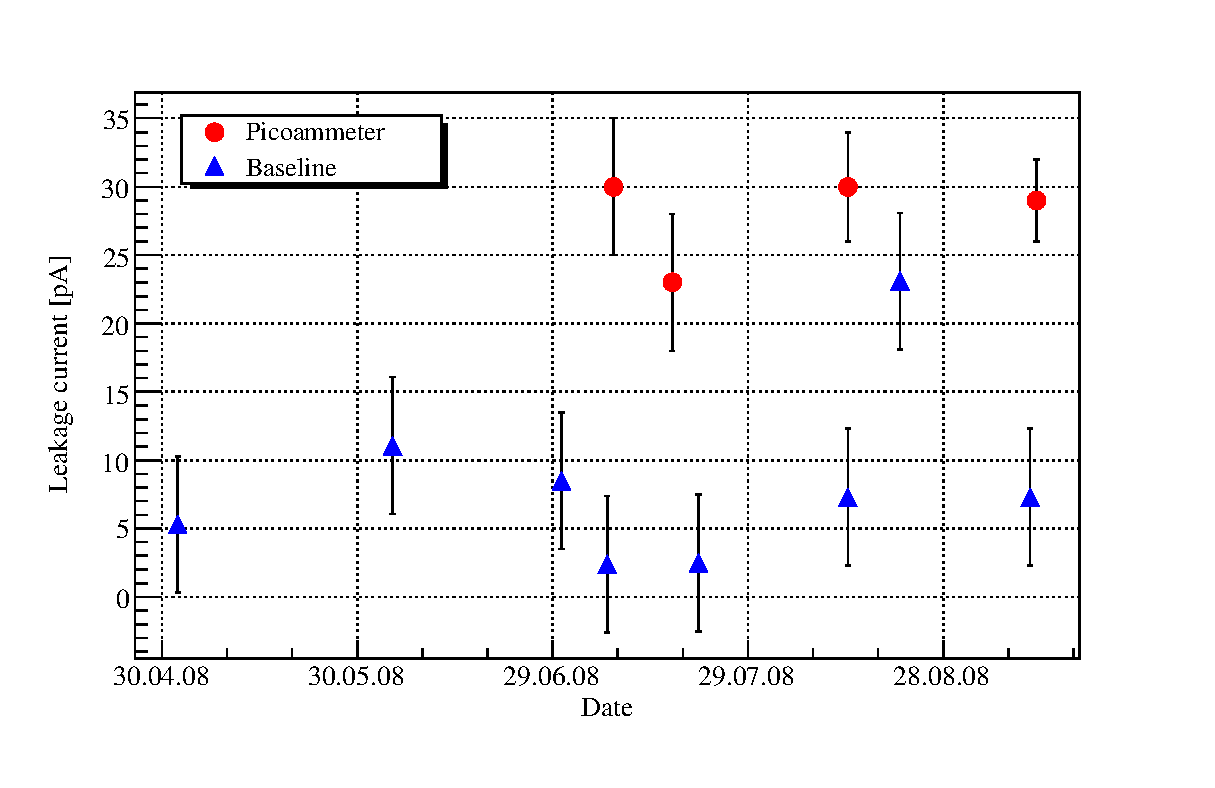
\includegraphics[width=0.6\textwidth, clip]{LC}
\caption{Leakage current of Siegfried II at 2000~V. Two different measurement methods were used. The first was to use a peco-amparemeter to directly measure the leakage current at 2000~V. The second was to compare the baselines of pulses at 0~V and 2000~V.}
\label{fig:ii:lc}
\end{figure}

Siegfried I was mounted to the middle detector mounting position in GII after the first warming-up of Siegfried II. Aferwards, four cooling-down and warming-up cycle were performed. Leakage currents of Siegfried I and II at operation voltage after each cooling-down were measured as shown in Fig.~\ref{fig:ii:lcs1} and \ref{fig:ii:lcs2}, respectively. The immediate measurements after each cooling-down showed dramatic increase of the leakage current. However, the leakage current kept dropping until reaching a constant value within around 40 minutes after the cooling-down. The measurements after that showed no increase of leakage current. This indicates some increase of the capacitance of the contacts between the detector surfaces and the signal cables.

\begin{figure}[htbp]
\centering
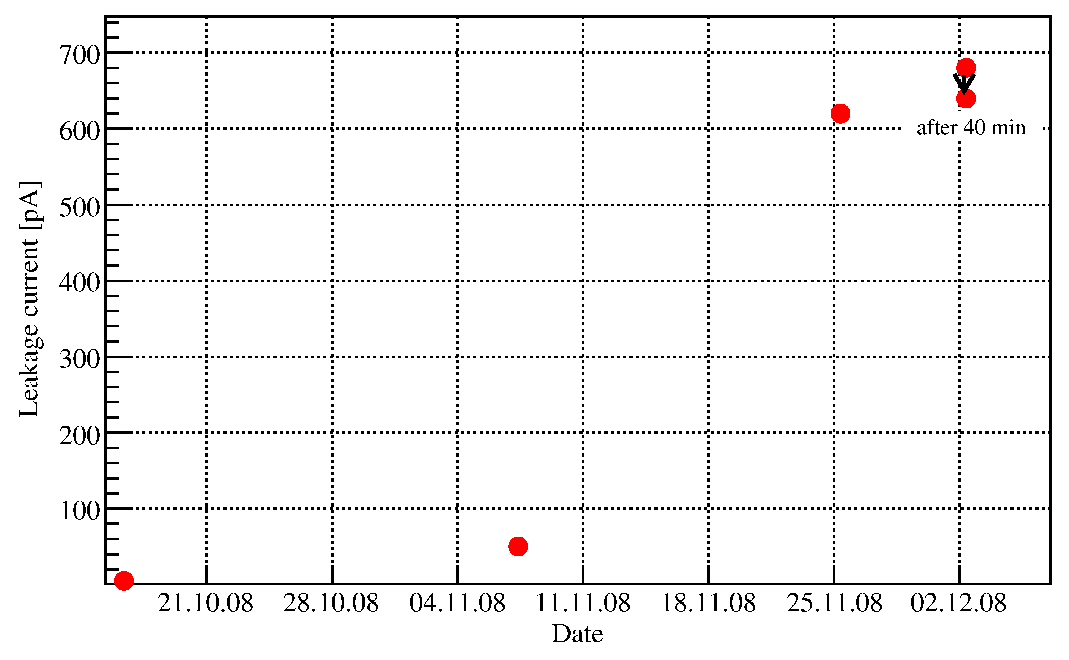
\includegraphics[width=0.6\textwidth]{LCs1}
\caption{Leakage current of Siegfried I at 3000~V right after each cooling-down. The current was directly measured using a peco-amparemeter.}
\label{fig:ii:lcs1}
\end{figure}

\begin{figure}[htbp]
\centering
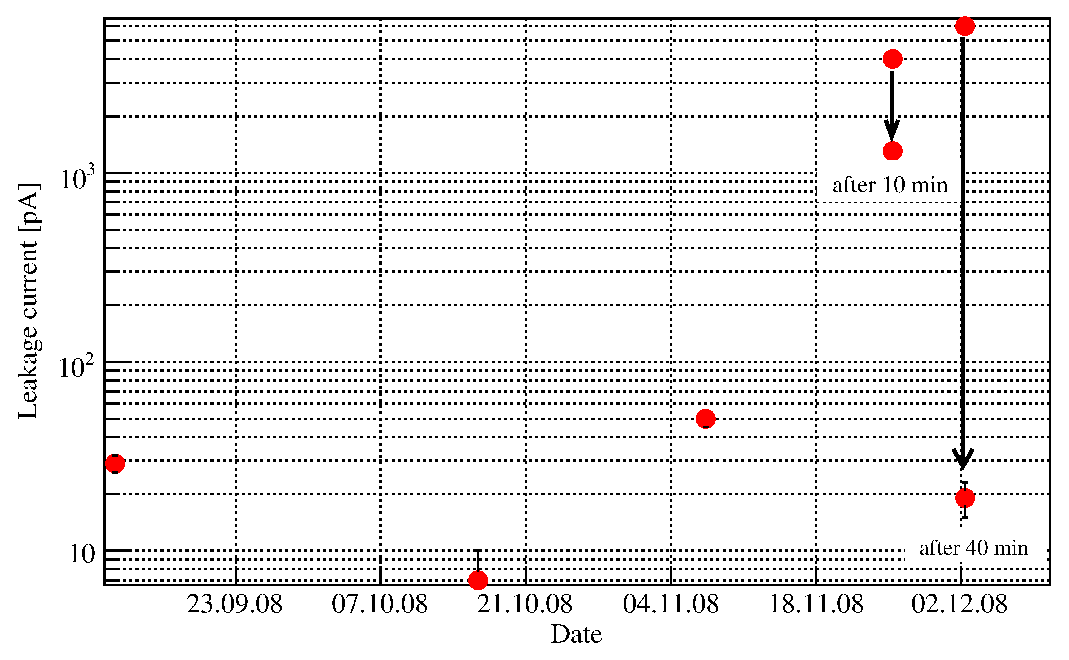
\includegraphics[width=0.6\textwidth, clip]{LCs2}
\caption{Leakage current of Siegfried II at 2000~V after each cooling-down. The current was directly measured using a peco-amparemeter.}
\label{fig:ii:lcs2}
\end{figure}

% \section{Capacitance measurement}
% \label{sec:ii:c}

% \section{Cross talk}
% \label{sec:ii:xtalk}
% with siegfried-II mounted.  The HV cable was connected through the HV feedthrough built on the top flange.  The shield of the HV cable was connected to the top flange.  Under the flange (thus inside the dewar) non-shielded Habia cable (?) was used for both the HV cable and the signal cables for the 18 segments.  A 2.2~nF capacitor and 1~G$\Omega$ resistor were used for the HV filter.  Another 2.2~nF capacitor was used for the core AC coupling. The two capacitors and the resistor were positioned right below the top flange, thus not inside the liquid Nitrogen and only in the gas Nitrogen enviroument.

\section{Negative pulse}
\label{sec:ii:npulse}
The preamplifiers and DAQ system were configured such that all the channels had positive polarity, \textit{i.e.}, the signals were positive pulses. About 10\% of the events were found to have negative pulses in some of the segments. Figure~\ref{fig:ii:npul} shows a typic negtive pulse event. It was a single-segment event, namely, there was only one segment (segment 2) having energy deposited. Segment 2 had a positive pulse. Transient pulses were induced in its neighboring segments 1 and 3. It is shown clearly that the baseline of the pulse in segment 3 dropped, which made it look like a negtive pulse.

\begin{sidewaysfigure}[htbp]
\centering
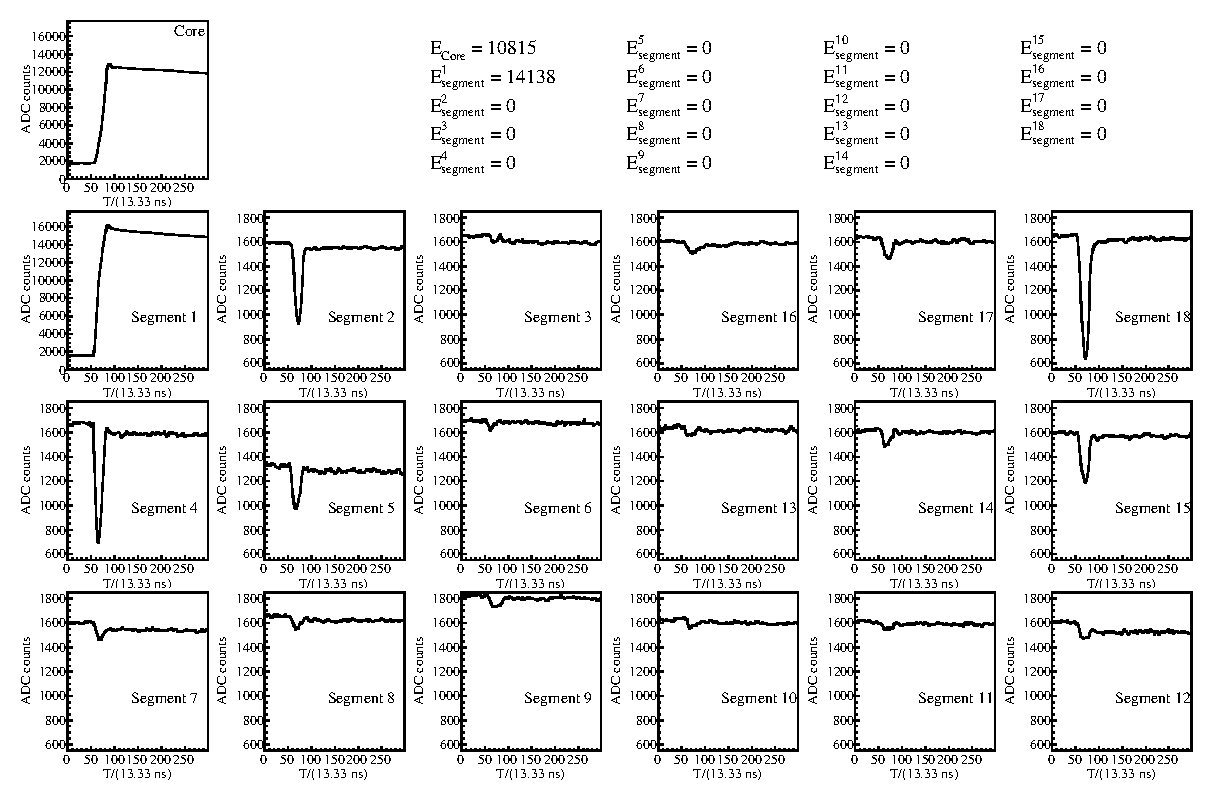
\includegraphics{npul}
\caption{An event showing negative pulse in one segment.}
\label{fig:ii:npul}
\end{sidewaysfigure}

\subsection{Selection of negtive pulse events}
\label{sec:ii:frac}
The sum of energies from all the segments, $\sum E_{\text{segment}}$, (including those with negtive pulses. They gave negative values.) agrees with the core energy, $E_{\text{core}}$, within the resolution. However, since the DAQ system estimated the energy of a negative pulse to be zero (as shown in the top right part of Fig.~\ref{fig:ii:npul}), the sum of the segment energies as calculated by DAQ, $\sum E^{\text{DAQ}}_{\text{segment}}$, was larger than $E_{\text{core}}$. By comparing  $\sum E^{\text{DAQ}}_{\text{segment}}$ and $E_{\text{core}}$, negative pulse events were identified and selected.

Figure~\ref{fig:ii:sEnegPulse} shows $\sum E^{\text{DAQ}}_{\text{segment}}$ versus $E_{\text{core}}$ of a data sample collected with an $^{228}$Th source mounted inside GII on top of Siegfried II. The two solid lines in the plot indicate the 20$\sigma$ range of the core energy. Points above the upper solid line correspond to the negative pulse events because they have $\sum E^{\text{DAQ}}_{\text{segment}} \gg E_{\text{core}}$. There is also a very small fraction of events with$\sum E^{\text{DAQ}}_{\text{segment}} < E_{\text{core}}$. This is due to the noise or pile-up\footnote{Two pulses are too close to each other in time for DAQ to get a correct estimation of energy.} effect. The fraction of negative pulse events is about 10\%.

\begin{figure}[tphb]
\centering
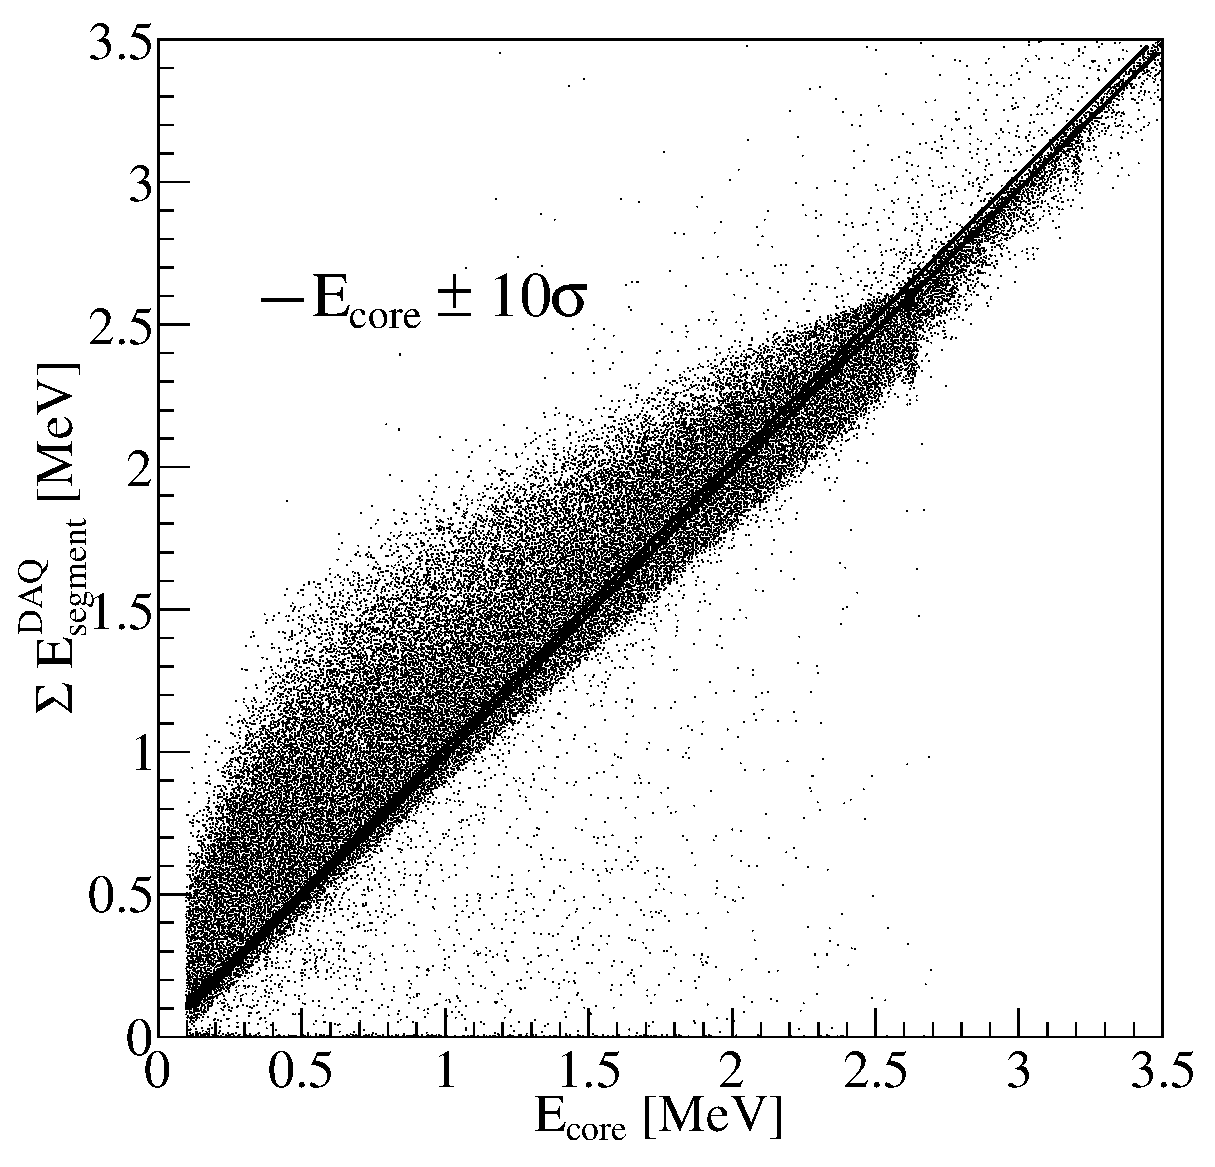
\includegraphics[width=0.5\textwidth]{sEnegPuls}
\caption{Sum of energies from all segments versus the core energy. All energies were calculated by the DAQ system. The two solid lines indicate the 20$\sigma$ range of the core energy.}
\label{fig:ii:sEnegPulse}
\end{figure}

\subsection{Location of negative pulse events}
\label{s:locneg}
To figure out the location of the negative pulse events, the energies from individual segments were plotted versus the core energy as shown in Fig.~\ref{f:ii:EnegPulse}. The two solid lines in the plot indicate the 20$\sigma$ range of the core energy. Negative pulse events were featured with  $E_{\text{segments}} > E_{\text{core}}$. They mainly populated in the segments on the top and bottom of the detector. Very few negative pulse events were found in the segments in the middle of the detector.

\begin{sidewaysfigure}[tphb]
\centering
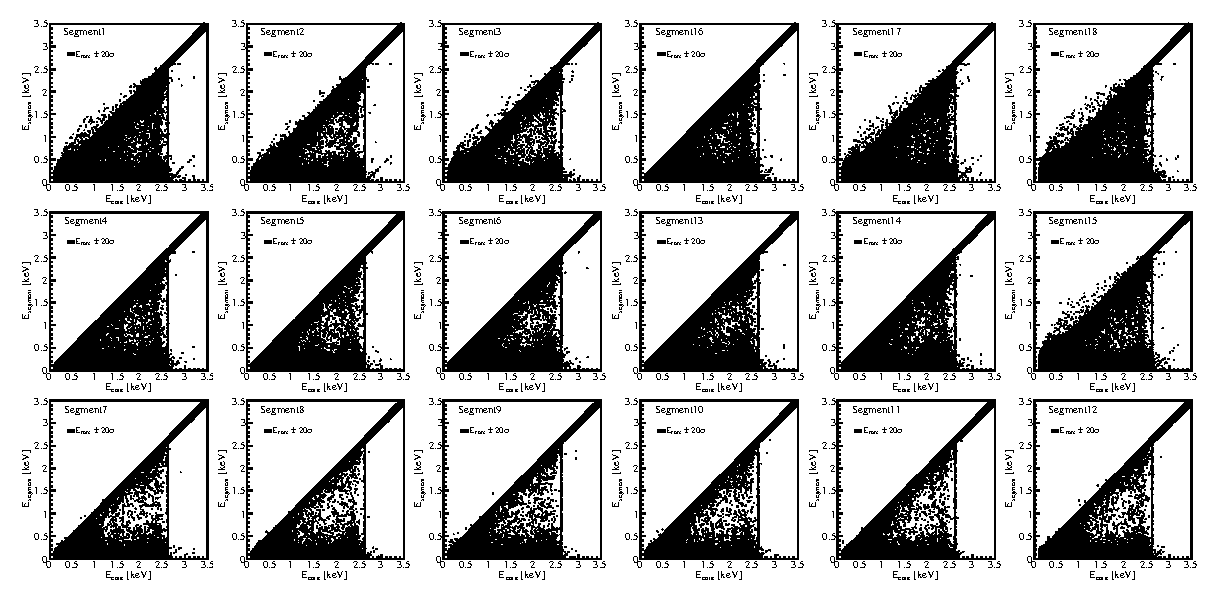
\includegraphics{EnegPuls}
\caption{Energies of individual segments versus the core energy. All energies were calculated by the DAQ system. The two solid lines in each plot indicate the 20$\sigma$ range of the core energy.}
\label{f:ii:EnegPulse}
\end{sidewaysfigure}

\subsection{Possible explanation}
\label{s:ii:exp}
The fact that the negative pulse events populated mainly in the top and bottom segments of the detector indicates that there might be surface channels~\cite{Sur05} formed, where the electric field was distorted and the rise time of the pulse increased subsequently. The DAQ energy filter could not handle the pulse with long rise time correctly and give an energy slightly smaller than the full energy. This would enhance the event rate on the low energy side of a full-energy peak at the cost of the peak itself. This was seen in Fig.~\ref{fig:ph:mca}: the low energy side of the 1332~keV peak in data is significantly higher than that in simulation in which the surface channel effect was not taken into account.

However, if the assumption was true, the fraction of negative pulse events in the low energy photon peaks should be larger than the fraction in the high energy photon peaks. Because low energy photons have a higher probability of depositing their energies close to the detector surface, while photons with higher energy are expected to penetrate deeper into the detector. Events within six photon peaks from the $^{228}$Th energy spectrum were selected to examinate the assumption. They are 239~keV from $^{212}$Pb, 583~keV from $^{208}$Tl, 861~keV from $^{208}$Tl, 2615~keV from $^{208}$Tl and its double- and single-escape peak 1592~keV and 2103~keV. For each of these 6 sub data samples the fractions of events with $\sum E_{\text{segment}} - E_{\text{core}} \gtrsim 20\sigma$ were calculated and plotted as a function of the core energy, as shown in Fig.~\ref{f:fnp_e}. No obvious correlation was found. The assumption hence needs to be studied further more. 

\begin{figure}[tphb]
\centering
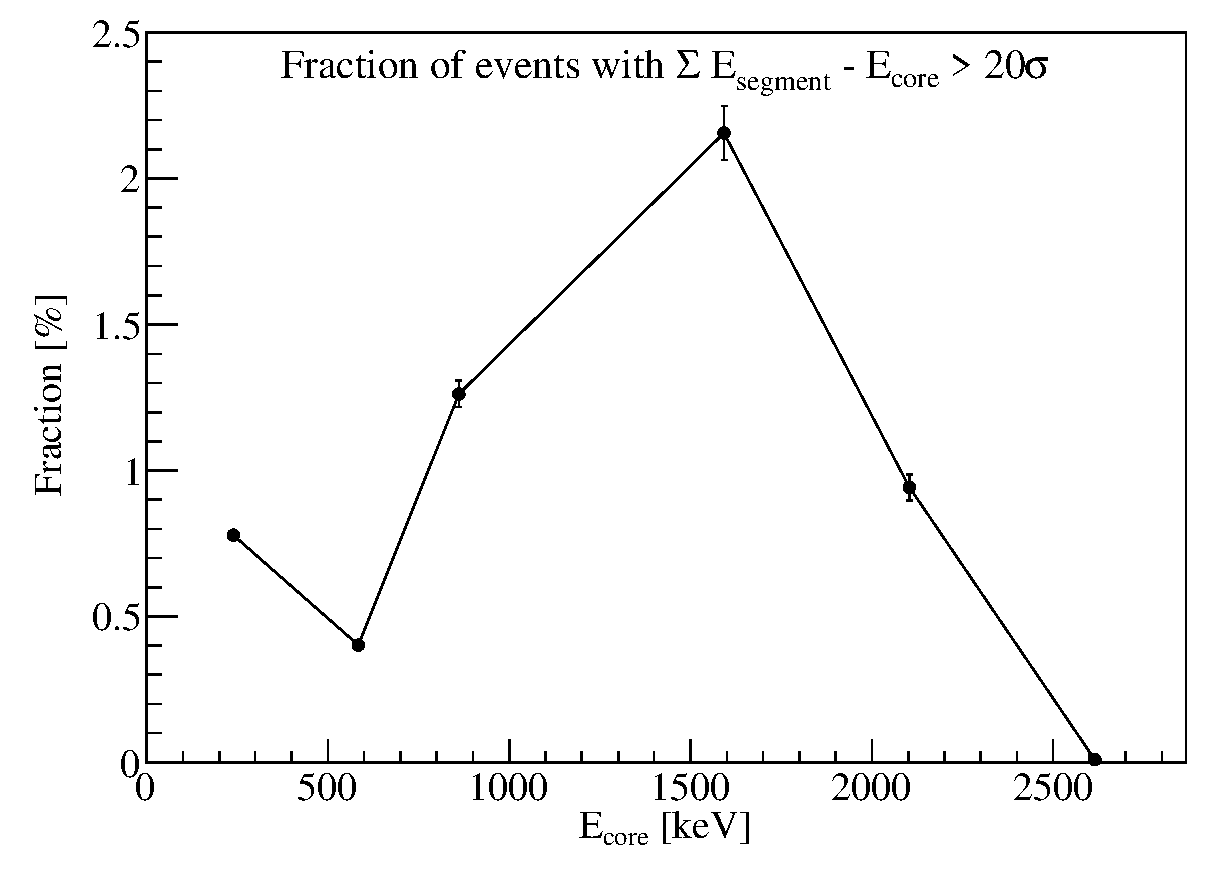
\includegraphics[width=0.6\textwidth]{fnp_e}
\caption{Fraction of events with $\sum E_{\text{segment}} - E_{\text{core}} \gtrsim 20\sigma$ as a function of core energy.}
\label{f:fnp_e}
\end{figure}

\section{Summary}
\label{sec:ii:sum}
A long term operation of Siegfried II directly in liquid nitrogen was performed using GII. Main performance parameters, such as resolution and leakage current, etc., were constantly monitored. Siegfried I was inserted into GII after the first warming-up of Siegfried II. They went through four cooling-down and warming-up cycles together. No obvious decrease of the performance was found. A small fraction of events taken with this setup were found to have negative pulses. Possible explanations were examined. Further investigation are needed.


%%% Local Variables:
%%% mode:latex
%%% TeX-master: "thesis"
%%% End:

\clearpage{\pagestyle{empty}\cleardoublepage}

\chapter{Neutron induced background}
\label{cha:neutron}
%$Id$



%%% Local Variables:
%%% mode:latex
%%% TeX-master: "thesis"
%%% End:


\chapter{Pulse shape simulation}
\label{cha:pss}
\chapter{Pulse shape simulation}
\label{cha:pss}
How segmentation can be used to distinguish between single- and
multi-segment events and how to use this information was described in
chapters~\ref{cha:photon} and~\ref{cha:neutron}.  However, as was
shown in Fig.~\ref{fig:ph:eve}, (1) there are some multi-site events
which are confined to one segment and (2) there are some single-site
events that happen on the boundary between two segments. If the
signal is identified with single-segment events, events from
category~(1) are counted erroneously as signal and events from
category~(2), \textit{boundary events}, are rejected erroneously,
because the energy deposited is shared between segments.

The analysis of the electrical pulses associated with the events
(pulse shape analysis) can help with both problems\footnote{Pulse
shape analysis can also help with several other aspects: rejection of
background from $\alpha$-particle and neutron interactions with
detectors, Compton continuum suppression\cite{comcon}, detection of
crystal structure~\cite{agata}, etc.}. For category (1) the time
development of the pulse can reveal a multi-site event while for
events in category (2) a close to equal strength and time development
of the two pulses can reveal its true single-site structure.
Concerning (1), previous studies \cite{Kev07} indicate that pulse
shape analysis can provide an extra suppression factor of 1.3 beyond
the suppression achieved through segment information alone. These
studies were limited by the lack of knowledge about the development of
the pulses in the detector and the electronic system.

Pulses resembling the ones expected for the $0\nu\beta\beta$ signal
are usually collected using photon induced events with a similar event
topology. Two data samples commonly used are (A) double escape peak
(DEP) events and (B) single Compton scattering
events\cite{scoms}. However, the double escape peaks are normally not
located near the $Q$-value of $^{76}$Ge $0\nu\beta\beta$ decay. In
addition, the events from the peak are not uniformly distributed
throughout the detector crystal \cite{major}.  Events from single
Compton scattering could, in principle, be selected to overcome these
restrictions. However, it is intrinsically difficult to collect large
such samples. Therefore, it is essential to supplement the data with
simulated pulses from a reliable simulation.

The physics models used for the drift of electrons and holes inside
germanium crystals were established by L. Mihailescu \textit{et
al.}\cite{miha} and B. Bruyneel \emph{et al.} \cite{bart},
respectively. The implementation of these models for Siegfried-like
detectors is described in detail in this chapter.


\section{Procedure}
\label{sec:pss:proc}
The procedure to simulate pulse shapes \cite{agata} is as follows:
\begin{enumerate} 
\item Simulate the interactions of particles with germanium using
Geant4 to get the spatial distribution and the energy deposits of the
interactions (hits);
\item Group hits if they are closer to each other than 1~mm. The
position of the new hit is the barycenter of the energies of the
original hits. The energy of the new hit is the sum of the energies of
the original hits.
\item Calculate the number of electron-hole pairs, $n$, created by the
hit with energy $E_{\text{hit}}$: $n = E_{\text{hit}} /
E_{\text{pair}}$, where the pair energy $E_{\text{pair}} = 2.95$~eV;
\item Get the electric field and the weighting potentials by
interpolating values at the neighboring grid points. The grid is
calculated once beforehand according to the high voltage applied and
the spatial distribution of the impurity. \cite{Gat82, Rad88, He00}
\item Calculate the drift velocities of the charge carriers taking
into account the effect of the crystal structure;
\item Calculate the trajectory of the drift from the interaction point
to the boundary of the crystal;
\item Calculate the time development of the charges induced in the
electrodes, namely, the pulses \cite{igex}. A dominant pulse is seen
in the electrode of the segment hit. However, other electrodes also
show pulses, so called mirror pulses, which also have to be simulated.
\item Add to the simulated pulses the effects from the electronics
such as noise, bandwidth limit, and shaping, etc.
\end{enumerate} 
MaGe, the object-oriented simulation package co-developed by the GERDA
and Majorana MC groups described in Sec.~\ref{sec:ph:sim} covers the
complete procedure. Step 5-7 were developed as part of this
thesis. The calculation of the electric fields and potentials is
described in Sec.~\ref{sec:pss:field}, the calculation of the drift
velocities of the charge carriers in Sec.~\ref{sec:pss:drift}.
 
 
\section{Electric and weighting fields} 
\label{sec:pss:field} 
The electric field $\mathbf{E}$ could, in principle, be calculated by
solving analytically Poisson's equation $\nabla \cdot \mathbf{E} =
\frac{\rho}{\epsilon}$ as described in Sec.~\ref{sec:det:field}. It is
more practical to numerically calculate the potential field
$\varphi$. The electric field $\mathbf{E}$ is then obtained using
$\mathbf{E} = - \nabla \varphi$. Since true coaxial detectors are
used, it is convenient to use cylindrical coordinates, $r, \phi, z$:
\begin{equation} 
\frac{1}{r} \frac{\partial \varphi}{\partial r} + \frac{\partial^{2} \varphi}{\partial r^{2}} + \frac{1}{r^{2}} \frac{\partial^{2} \varphi}{\partial \phi^{2}} + 
\frac{\partial^{2} \varphi}{\partial z^{2}} = - \frac{1}{\epsilon_{0} 
\epsilon_{R}} \rho, 
\label{eq:pss:pocyl} 
\end{equation} 
where $\varphi$ and $\rho$ are functions of $r, \phi, z$;
$\epsilon_{0}$ and $\epsilon_{R}$ are the dielectric constants in
vacuum and germanium, respectively.
 
The electric field distribution inside the germanium crystal is quite
sensitive to the impurity density. Figure~\ref{fig:pss:rho} shows the
strength of the electric field as a function of $r$ with the bias
voltage fixed at 3~kV.  A change of the impurity density by one order
of magnitude changes the electric field dramatically. Even a factor
three difference, usually allowed between top and bottom for a
commercial detector, has a very significant effect.

 
\begin{figure}[htbp] 
\centering 
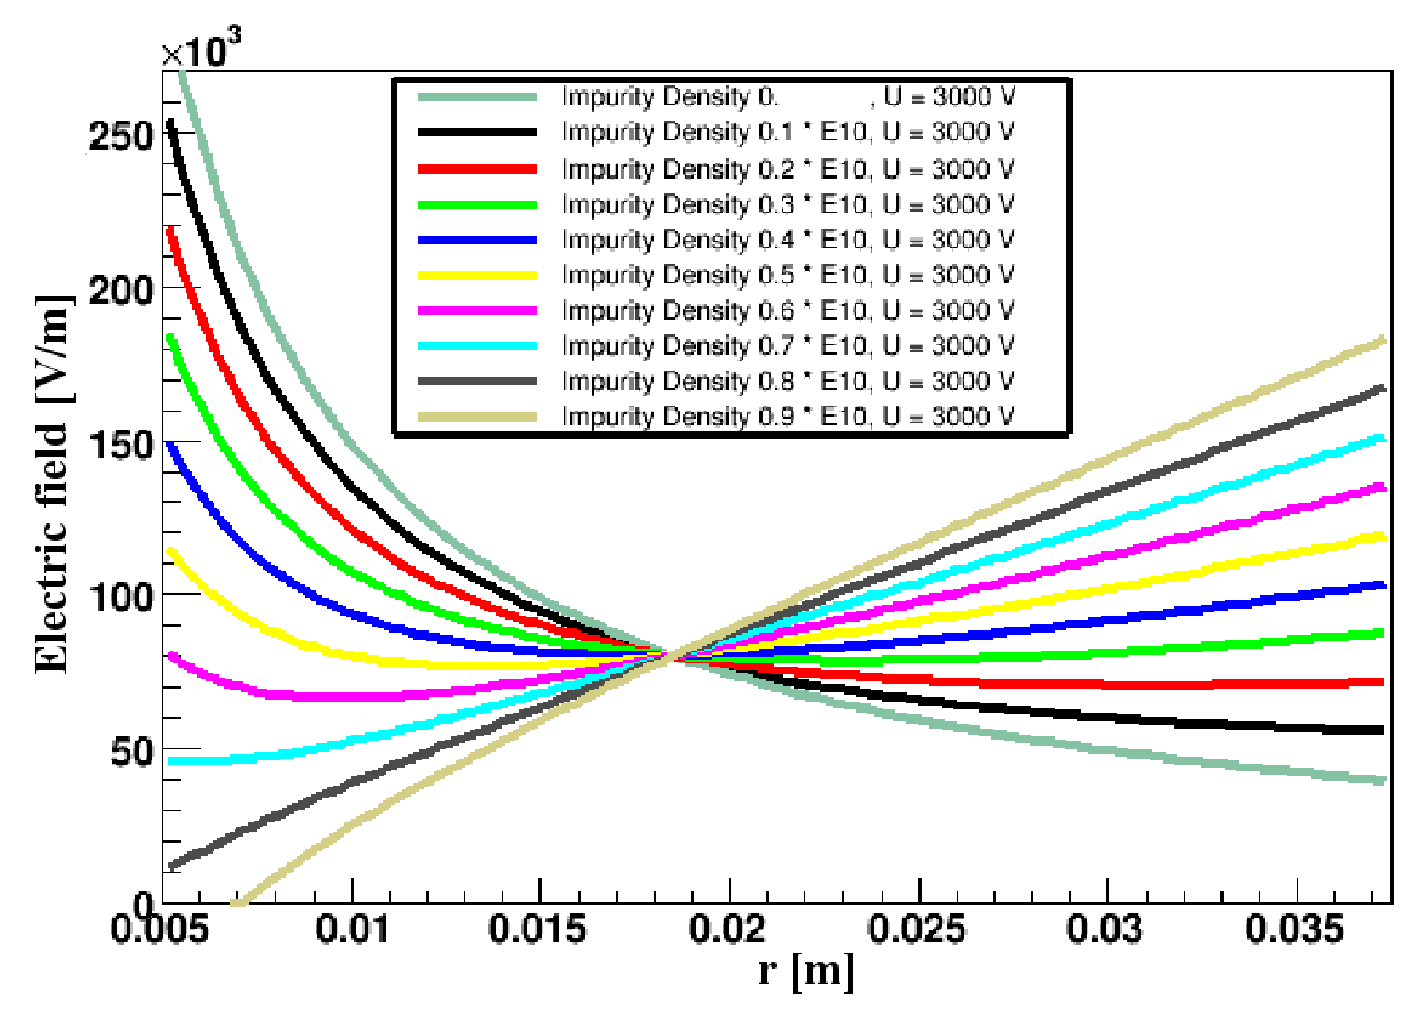
\includegraphics[width=0.65\textwidth]{rho} 
\caption{Strength of the electric field as a function of the
cylindrical coordinate $r$ for impurity densities between 0 and $0.9
\times 10^{-10}$/cm$^{3}$.}
\label{fig:pss:rho} 
\end{figure} 
 
The weighting fields and potentials are calculated in the same way to
determine the signals induced in the electrodes using Shockley-Ramo's
Theorem \cite{Gat82, Rad88, He00} as described in
Sec.~\ref{sec:det:ramo}.
 
 
\section{Drift of charge carriers} 
\label{sec:pss:drift} 
 
\subsection{Mobility} 
\label{sec:pss:mobi} 
The electrons and holes drift to the electrodes of the detector. The
mobilities of electrons $\mu_{e}$ and holes $\mu_{h}$ as defined in
Sec.~\ref{sec:det:struc} change with the temperature of the germanium
crystal. If the temperature of electrons and holes\footnote{If the
velocities of a group of electrons or holes follow a Maxwell-Boltzmann
distribution, their temperature is defined as the temperature of that
distribution.} do not differ much from the temperature of the crystal
lattice, the drift velocity $\mathbf{v}_{e/h}$ is simply proportional
to the electric field and the crystal structure has no
influence. The mobility in this case is just a number,$\mu_{0}$. As
germanium detectors are operated at $\approx 100$~K, the electrons and
holes are hotter than the crystal lattice. The mobility in this case
depends on the crystal orientation and is a complex tensor. The drift
trajectory, hence, is not always parallel to the electric field.
 
Germanium has the same crystalline structure as silicon and diamond,
\textit{i.e.} a face-centered cubic (FCC) structure: each atom is at
the center of a regular tetrahedron and is surrounded by four atoms as
shown in Fig.~\ref{fig:pss:xtal}. Also shown is the definition of
crystal axes in terms of the Miller index.
 
\begin{figure}[tbhp] 
\centering 
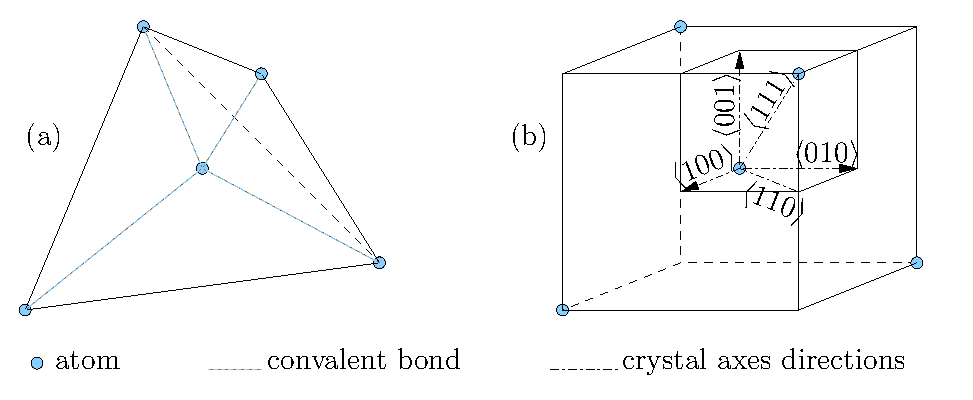
\includegraphics[width=0.8\textwidth]{xtalStruc}   
\caption{Structure of germanium crystals: (a) basic configuration and
(b) definition of crystal axes.}
\label{fig:pss:xtal} 
\end{figure} 
 
If the electric field lines are parallel to any of the three principal
crystallographic axes $\langle 100 \rangle$, $\langle 110 \rangle$ and
$\langle 111 \rangle$, the charge carriers will drift along the
electric field because of the symmetric structure of the germanium
crystal. In this case the drift velocity only depends on the strength
of the electric field. Measurements of the drift velocities along the
axes $\langle 100 \rangle$ and $\langle 111 \rangle$ with electric
field parallel to them were performed and the data can be fitted well
by the following parametrization \cite{Kno99}:
\begin{equation} 
\label{eq:pss:para} 
v = \frac{\mu_{0}E}{[1+(\frac{E}{E_{0}})^{\beta}]^{1/\beta}} - \mu_{n}E, 
\end{equation} 
where $E, v$ are the magnitudes of the electric field and drift
velocity, respectively, $\mu_{0}, \mu_{n}, E_{0}$ and $\beta$ are
parameters to be determined by fitting. The parameter $\mu_{0}$
represents a simple linear relation between $v$ and $E$. A deviation
from this linear relation occurs at low temperatures
($\approx$100~K). It is modeled through the parameters $E_{0}$ and
$\beta$. Mihailescu \textit{et al.} \cite{miha} added the term
$\mu_{n}E$ for electric fields stronger than 300~V/mm to account for
the \emph{Gunn effect} observed by Ottaviani \textit{et al.}
\cite{otta}. This effect is irrelevant here as our detectors are
operated at field strengths well below 300~V/mm. The values of the
parameters of the fit to the experimental data are listed in
Table~\ref{tab:pss:pars}. They are an important input for the
simulation presented here.
 
\begin{table}[tbhp] 
\centering 
\caption{Parameters for the experimental drift velocities in the 
$\langle111\rangle$ and $\langle 100 \rangle$ directions 
(taken from Ref.~\cite{bart}).} 
\label{tab:pss:pars}
\begin{tabular*}{\textwidth}{ccccccc}\hline\hline 
Reference & Carrier & Direction & $\mu_{0} \left[ \frac{\mbox{cm}^{2}}{\mbox{V}\cdot\mbox{s}} \right]$ & $E_{0} \left[ \frac{\mbox{V}}{\mbox{mm}} \right]$ & $\beta$ & $\mu_{n} \left[ \frac{\mbox{cm}^{2}}{\mbox{V}\cdot\mbox{s}} \right]$ \\\hline 
& Electrons & $\langle111\rangle$ & 40180 & 49.3 & 0.72 & 589 \\ 
Ref.~\cite{miha}& & $\langle100\rangle$ & 42420 & 25.1 & 0.87 & 62\\ 
& Holes & $\langle111\rangle$ & 107270 & 10.0 & 0.58 & 0 \\ 
& & $\langle100\rangle$ & 66333 & 18.1 & 0.744 & 0 \\\hline 
& Electrons & $\langle111\rangle$ & 38536 & 53.8 & 0.641 & 510 \\ 
Ref.~\cite{bart}& & $\langle100\rangle$ & 38609 & 51.1 & 0.805 & -171\\  
& Holes & $\langle111\rangle$ & 61215 & 18.2 & 0.662 & 0 \\ 
& & $\langle100\rangle$ & 61824 & 18.5 & 0.942 & 0 \\\hline\hline 
\end{tabular*} 
\end{table} 
 
Figure~\ref{fig:pss:vvse} shows the drift velocities of electrons (a,
c) and holes (b, d) along the principal crystal axes as functions of
electric field in the range of [7,500]~V/mm. The drift velocities
along the $\langle 100 \rangle$ and $\langle 111 \rangle$ axes were
calculated according to Eq.~\ref{eq:pss:para}. The input parameters
provided in Ref.~\cite{miha} (\cite{bart}) were used for
Fig.~\ref{fig:pss:vvse}a and b (c and d).  The drift velocity in any
direction can be derived from the velocities along the $\langle 100
\rangle$ and $\langle 111 \rangle$ axes.  The details of the
calculation are described in the following sections.
 
\begin{figure}[tbhp] 
\centering 
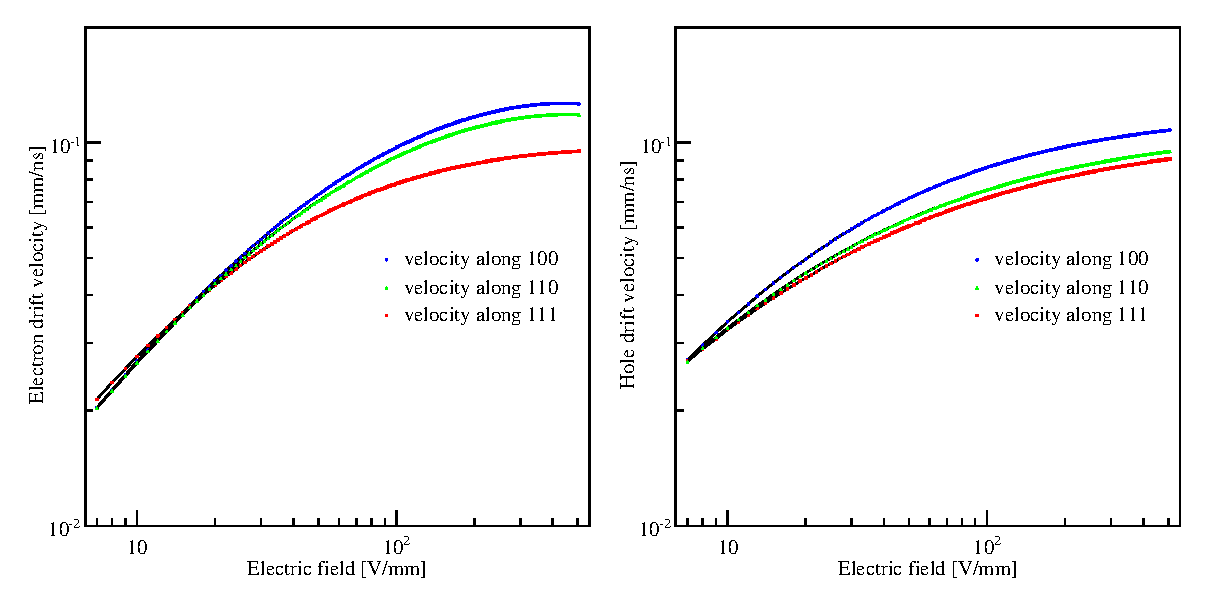
\includegraphics[width=\textwidth]{VvsElucian} \\\hfil 
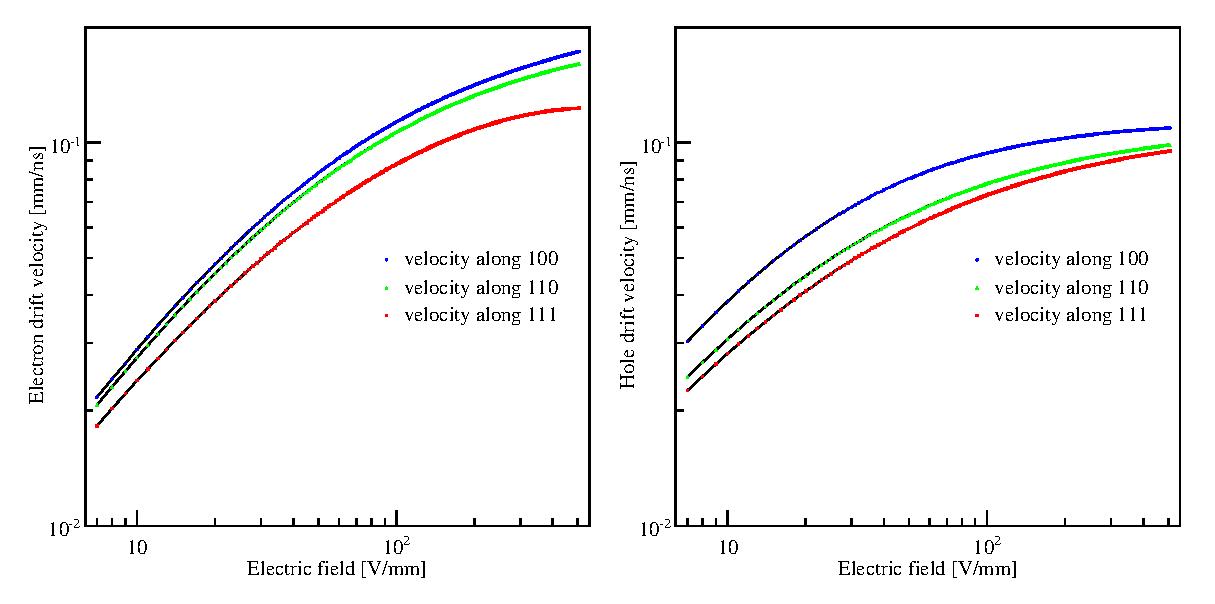
\includegraphics[width=\textwidth]{VvsEbart} 
\caption{Drift velocities of electrons (a, c) and holes (b, d) along
the principal crystal axes as functions of electric field in the range
of [7,500]~V/mm. Velocities along the axes $\langle 100 \rangle$ and
$\langle 111 \rangle$ were calculated according to
Eq.~\ref{eq:pss:para}: (a) and (b), the input parameters provided in
Ref.~\cite{miha} were used; (c) and (d), the input parameters provided
in Ref.~\cite{bart} were used. The velocities along the $\langle 110
\rangle$ axis are predicted according sections~\ref{sec:pss:elec}
and~\ref{sec:pss:hole}.}
\label{fig:pss:vvse} 
\end{figure} 
 
\subsection{Coordinate systems} 
\label{sec:pss:xyz} 
Two different coordinate systems are important for the
calculation. The first one is defined by the crystal axes $\langle 100
\rangle$, $\langle 010 \rangle$ and $\langle 001 \rangle$. The second
one, indicated as $xyz$ in Fig~\ref{fig:pss:coo}, is used in
Geant4. The cylindrical detectors are produced with their geometrical
middle axis, $z$, aligned to the crystal axis $\langle 001
\rangle$. The transformation between the two coordinate system, hence,
only depends on the angle between the $\langle 110 \rangle$ and the
y-axis, $\phi_{110}$.
\begin{SCfigure}[1.1][t!] 
\centering 
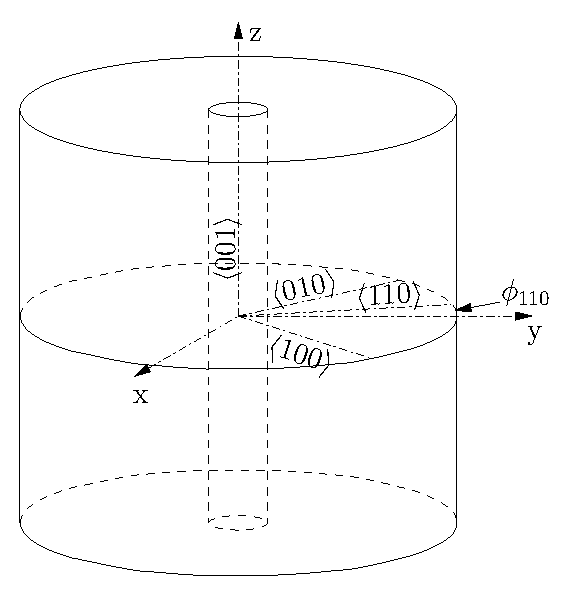
\includegraphics[width=0.4\textwidth]{coordins}   
\caption{The relation between the coordinates $xyz$ used in Geant4 and
the crystal axes $\langle 100 \rangle$, $\langle 010 \rangle$ and
$\langle 001 \rangle$.}
\label{fig:pss:coo} 
\end{SCfigure} 
 
\subsection{Electron drift velocity} 
\label{sec:pss:elec} 
The conduction band in a germanium crystal reaches its minimal
potential in regions around the four equivalent $\langle 111 \rangle$
axes. The equipotential surfaces in these regions have ellipsoidal
shapes as shown in Fig~\ref{fig:pss:valley}.
\begin{SCfigure}[1.2][b!] 
\centering 
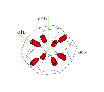
\includegraphics[width=0.4\textwidth]{valleys}   
\caption{Minimal potential regions in the conduction band along four
equivalent $\langle 111 \rangle$ axes, where the probability density
of electrons is dominant (taken from Ref.~\cite{bart}).}
\label{fig:pss:valley} 
\end{SCfigure} 
These regions are characterized by valleys in the conduction band
which can easily be populated by free electrons. The electrons have a
high mobility and are strongly accelerated by the electric field
applied.  The probability density of conduction band electrons in
other regions is very small. If it is neglected, the dependence of the
electron drift velocity $\mathbf{v}_{e}$ on the applied electric field
$\mathbf{E}$ can be written as
\begin{equation} 
\label{eq:pss:ed} 
\mathbf{v}_{e}(\mathbf{E}) = \mathcal{A}(E) \sum_{j} \frac{n_{j}}{n} 
\frac{\gamma_{j}\mathbf{E_{0}}}
{\sqrt{\mathbf{E_{0}}^{T}\gamma_{j}\mathbf{E_{0}}}}, 
\mbox{ with } j=1,2,3,4, 
\end{equation} 
where the coefficient $\mathcal{A}$ is a function of $E=|\mathbf{E}|$
and the temperature; $\mathbf{E_{0}}$ is the normalized electric field
vector; $n_{j}/n$ is the fraction of the carriers (in this case,
electrons) in the $j$-th $\langle 111 \rangle$ valley and $\gamma_{j}$
is the effective mass tensor for the electrons in the $j$-th $\langle
111 \rangle$ valley. Local coordinates,
$x^{\prime}y^{\prime}z^{\prime}$, are defined as shown in
Fig.~\ref{fig:pss:axes}. The effective mass tensor, $\gamma_{0}$, in
$x^{\prime}y^{\prime}z^{\prime}$ coordinates has a very simple
expression:
\begin{equation} 
\label{eq:pss:g0} 
\gamma_{0} \equiv \left( 
\begin{array}{ccc} 
m_{t}^{-1} & 0 & 0 \\ 
0 & m_{l}^{-1} & 0 \\ 
0 & 0 & m_{t}^{-1} 
\end{array} \right), 
\end{equation} 
where $m_{t} = 1.64m_{e}$ is the transverse effective electron mass
and $m_{l} = 0.0819m_{e}$ is the longitudinal effective electron mass,
with $m_{e}$ denoting the free electron mass. Since it is convenient
to simulate the interactions and the pulse shape development in the
$xyz$ coordinates, the expression of the mass tensor has to be
transformed from $x^{\prime}y^{\prime}z^{\prime}$ to $xyz$
coordinates:
\begin{equation} 
\label{eq:pss:gs} 
\gamma_{j} = R_{j}^{-1}\gamma_{0}R_{j} = R_{j}^{T}\gamma_{0}R_{j}, 
\end{equation} 
where 
\begin{equation} 
\label{eq:pss:rs} 
R_{j} = R_{x^{\prime}}(\arccos(\sqrt{2/3}))R_{z}(\phi_{110}+(j-1)\pi/2) 
\end{equation} 
is the rotation matrix which aligns one of the four $\langle 111
\rangle$ axes to the y-axis. $R_a(\alpha)$ indicates a
counter-clockwise rotation around the axis~$a$ with rotation
angle~$\alpha$.
 
\begin{SCfigure}[1.2][tbhp] 
\centering 
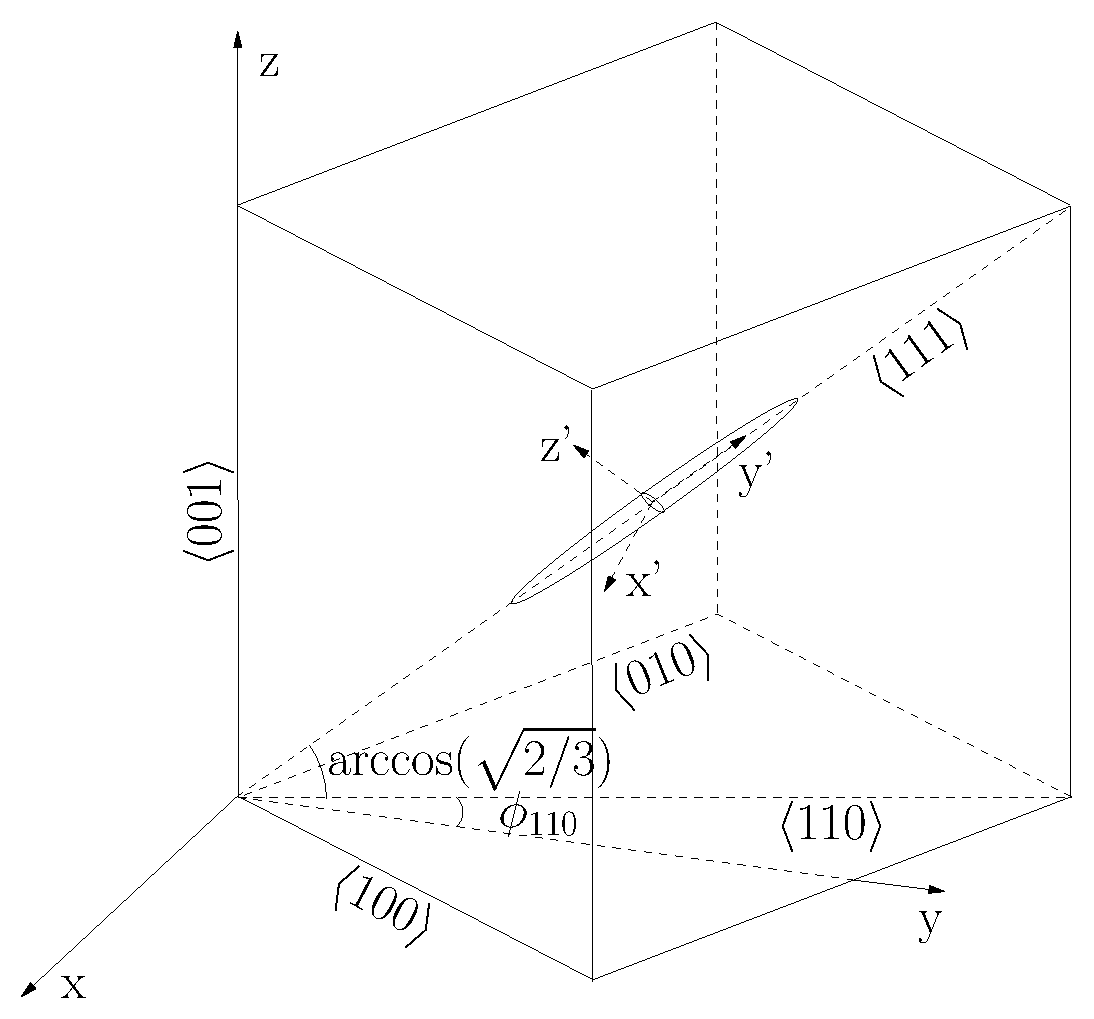
\includegraphics[width=0.4\textwidth]{axes}   
\caption{Relation between the local coordinates
$x^{\prime}y^{\prime}z^{\prime}$ in one of the four ellipsoidal
regions with conduction band valleys and the Geant4 coordinates
$xyz$. The $x^{\prime}$ axis is perpendicular to the plane defined by
$\langle111\rangle$ and $\langle001\rangle$.}
\label{fig:pss:axes} 
\end{SCfigure} 
 
The deviation from an equal population , i.e. $n_{e}/n$=1/4, of
electrons is assumed to depend on the electric field like:
\begin{equation} 
\label{eq:pss:nion} 
\frac{n_{j}}{n} = \mathcal{R}(E) 
\left[ \frac{\sqrt{\mathbf{E_{0}}^{T}\gamma_{j}\mathbf{E_{0}}}}
{\sum_{i}\sqrt{\mathbf{E_{0}}^{T}\gamma_{i}\mathbf{E_{0}}}} - 
\frac{n_{e}}{n} \right] + \frac{n_{e}}{n},  
\end{equation} 
where the coefficient $\mathcal{R}$ is a function of $E=|\mathbf{E}|$
and the temperature.
 
An electric field applied along the $\langle 100 \rangle$ direction,
\textit{i.e.} $\mathbf{E_{0}} = (\sqrt{1/2}, \sqrt{1/2}, 0)^{T}$ in
$xyz$ coordinates affects the population of the electrons in all
$\langle 111 \rangle$ valleys equally, hence $n_{1}/n = n_{2}/n =
n_{3}/n = n_{4}/n = 1/4$. Using the drift velocity $v_{e}^{100}(E)$
according to Eq.~\ref{eq:pss:para}, the absolute value of
$\mathcal{A}(E)$ can be expressed as
\begin{equation} 
\label{eq:pss:ae} 
|\mathcal{A}(E)| = \frac{v_{e}^{100}(E)}  
{\displaystyle \sum_{j} \frac{1}{4} \frac{\gamma_{j}\mathbf{E_{0}}}
{\sqrt{\mathbf{E_{0}}^{T}\gamma_{j}\mathbf{E_{0}}}}}, \mbox{ with } 
\mathbf{E_{0}} = \left( \begin{array}{c}  
\sqrt{1/2}\\\sqrt{1/2}\\0 \end{array} \right). 
\end{equation} 
 
If the electric field vector is oriented along one of the four
$\langle 111 \rangle$ axes, \textit{i.e.} $\mathbf{E_{0}} = (0,
\sqrt{2/3}, \sqrt{1/3})^{T}$ in $xyz$ coordinates, there is an uniform
population of the electrons among the other three $\langle 111
\rangle$ axes, \textit{i.e.}
\begin{equation} 
\label{eq:pss:n111} 
\frac{n_{2}}{n} = \frac{n_{3}}{n} = \frac{n_{4}}{n}. 
\end{equation} 
Since 
\begin{equation} 
\label{eq:pss:nsum} 
\displaystyle \sum_{j}\frac{n_{j}}{n} = 1, 
\end{equation} 
we have 
\begin{equation} 
\label{eq:pss:n12} 
\frac{n_{1}}{n} + 3\frac{n_{2}}{n}= 1. 
\end{equation} 
Using the drift velocity $v_{e}^{111}(E)$ for an applied electric
field $E$ in the $\langle 111 \rangle$ direction at a specific
temperature according to Eq.~\ref{eq:pss:para}, another relation
between $n_{1}/n$ and $n_{2}/n$ is obtained:
\begin{equation} 
\label{eq:pss:n12p} 
v_{e}^{111}(E) =  \mathcal{A}(E) 
\left( \frac{n_{1}}{n} \frac{\gamma_{1}\mathbf{E_{0}}} 
{\sqrt{\mathbf{E_{0}}^{T}\gamma_{1}\mathbf{E_{0}}}} +  
3\frac{n_{2}}{n} \frac{\gamma_{2}\mathbf{E_{0}}}         
{\sqrt{\mathbf{E_{0}}^{T}\gamma_{2}\mathbf{E_{0}}}} \right). 
\end{equation} 
The values of $n_{1}/n$ and $n_{2}/n$ can be obtained by solving the
equations \ref{eq:pss:n12} and \ref{eq:pss:n12p}. Then
$\mathcal{R}(E)$ can be calculated as
\begin{equation} 
\label{eq:pss:re} 
\mathcal{R}(E) = \left( \frac{n_{1}}{n} - \frac{n_{e}}{n} \right) / 
\left( \frac{\sqrt{\mathbf{E_{0}}^{T}\gamma_{1}\mathbf{E_{0}}}} 
{\sum_{j}\sqrt{\mathbf{E_{0}}^{T}\gamma_{j}\mathbf{E_{0}}}} - 
\frac{n_{e}}{n} \right), \mbox{ with } 
\mathbf{E_{0}} = \left( \begin{array}{c}  
0\\ \sqrt{2/3}\\\sqrt{1/3} \end{array} \right). 
\end{equation} 
 
After the determination of the coefficients $\mathcal{A}$ and
$\mathcal{R}$ the drift velocity can be calculated for any direction
and any strength of the electric field. Figures~\ref{fig:pss:vvse}a
and c present the calculated electron drift velocities along the
$\langle 110 \rangle$ axis. The velocities are between the ones for
the other axes.

 
\subsection{Hole drift velocity} 
\label{sec:pss:hole} 
The model used to calculate the hole drift velocity is taken from
Ref.~\cite{bart}. In this model only the \emph{heavy hole valence
band} is responsible for the anisotropy of the mobility. All other
effects are neglected. A hole is accelerated by the electric field
until its energy becomes 0.037~eV. At this point it is very likely to
emit an optical phonon and lose most of its energy, after which
acceleration in the field direction resumes and a new cycle starts.
 
The probability of finding a heavy hole in a specific momentum state
$\mathbf{k}$ is maximal in the direction parallel to the electric
field. The mean wave vector $\mathbf{k}_{0}(k_{0}, \theta_{0},
\phi_{0})$ is then assumed to be aligned with the electric field
$\mathbf{E}(E, \theta, \phi)$, namely, $\theta_{0} = \theta, \phi_{0}
= \phi$, where $\theta, \phi$ are the polar and azimuthal angles with
respect to the coordinate system defined by the $\langle 100 \rangle$,
$\langle 010 \rangle$ and $\langle 001 \rangle$ axes as shown in
Fig.~\ref{fig:pss:vsphere}.
 
\begin{SCfigure}[1.2][tbhp] 
\centering 
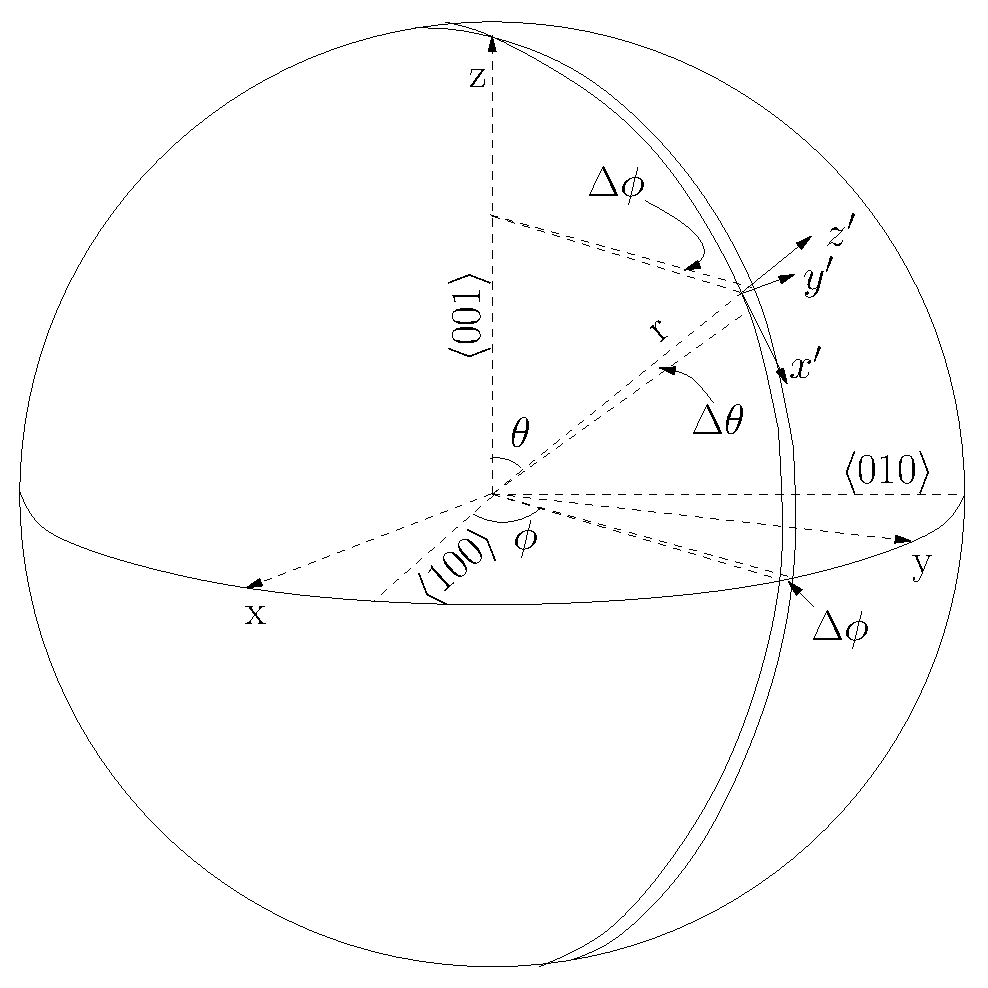
\includegraphics[width=0.4\textwidth]{vsphere}   
\caption{Relation between the crystal axes $\langle100\rangle$,
$\langle010\rangle$ and $\langle001\rangle$, and the coordinates $xyz$
used in Geant4, and the local coordinates
$x^{\prime}y^{\prime}z^{\prime}$.}
\label{fig:pss:vsphere} 
\end{SCfigure} 
 
The three components $(v_{x^{\prime}}, v_{y^{\prime}},
v_{z^{\prime}})^{T}$ of the hole drift velocity $\mathbf{v}$ in the
local coordinates, $x^{\prime}y^{\prime}z^{\prime}$, at any position
$(r, \theta, \phi)$ (as shown in Fig.~\ref{fig:pss:vsphere}) can be
expressed as:
\begin{equation} 
\label{eq:pss:vsphere} 
\begin{array}{rcl} 
v_{x^{\prime}} = v_{r} &=& v^{100}_{h}(E)[1-\Lambda(k_{0})(\sin(\theta)^{4}\sin(2\phi)^{2} + \sin(2\theta)^{2})],\\ 
v_{y^{\prime}} = v_{\theta} &=& v^{100}_{h}(E)\Omega(k_{0})[2\sin(\theta)^{3}\cos(\theta)\sin(2\phi)^{2} + \sin(4\theta)],\\ 
v_{z^{\prime}} = v_{\phi} &=& v^{100}_{h}(E)\Omega(k_{0})\sin(\theta)^{3}\sin(4\phi), 
\end{array} 
\end{equation} 
The mean wave number $k_{0}$ can be expressed as a function of
$v_{rel} = v^{111}_{h}(E)/v^{100}_{h}(E)$:
\begin{equation} 
\label{eq:pss:k0} 
k_{0}(v_{rel}) = 9.2652 - 26.3467v_{rel} + 29.6137v_{rel}^{2} - 12.3689v_{rel}^{3}, 
\end{equation} 
where $v^{111}_{h}(E)$ and $v^{100}_{h}(E)$ are the drift velocities
along the $\langle111\rangle$ and $\langle100\rangle$ axes. They can
be calculated using Eq.~\ref{eq:pss:para}. The magnitude of the
anisotropies, $\Lambda$ and $\Omega$, can be expressed as
\begin{equation} 
\label{eq:pss:lamb} 
\Lambda(k_{0}) = -0.01322k_{0} + 0.41145k_{0}^{2} - 0.23657k_{0}^{3} + 0.04077k_{0}^{4}, 
\end{equation} 
\begin{equation} 
\label{eq:pss:ome} 
\Omega(k_{0}) = 0.006550k_{0} - 0.19946k_{0}^{2} + 0.09859k_{0}^{3} - 0.01559k_{0}^{4}. 
\end{equation} 
 
The three components $(v_{x}, v_{y}, v_{z})^{T}$ of the hole drift
velocity $\mathbf{v}$ in $xyz$ coordinate (as shown in
Fig.~\ref{fig:pss:vsphere}) become:
\begin{equation} 
\label{eq:pss:v2v}   
\left( 
\begin{array}{c} 
v_{x} \\ v_{y} \\ v_{z} 
\end{array} 
\right) = R_{z}(\phi + \frac{\pi}{4} + \phi_{110}) R_{y^{\prime}}(\theta) \left(  
\begin{array}{c} 
v_{x^{\prime}} \\ v_{y^{\prime}} \\ v_{z^{\prime}} 
\end{array} \right), 
\end{equation} 
where $R_a(\alpha)$ indicates the counter-clockwise rotation around
the axes $a$ by the angle $\alpha$.  Figures~\ref{fig:pss:vvse}b and d
present the calculated hole drift velocities along the $\langle 110
\rangle$ axis. The velocities are between the ones along the other
axes.
 
 
\section{Drift trajectories } 
\label{sec:pss:trj} 
The trajectories are calculated iteratively.  The displacement vector
$\Delta \mathbf{r}$ by which a charge carrier drifts within a short
time interval $\Delta t$ can be calculated once the drift velocity
vector $\mathbf{v}_{i}$ in the original position $\mathbf{r}_{i}$ is
calculated using the method described in the previous two sections.
The new position $\mathbf{r}_{i+1}$ is then
\begin{equation} 
\label{eq:pss:pos} 
\mathbf{r}_{i+1} = \mathbf{r}_{i} + \Delta \mathbf{r} \ \ 
(i=0,1,...), \text{ with } 
\Delta \mathbf{r} = \mathbf{v}_{i} \Delta t. 
\end{equation} 
The iteration continues until the charge carriers reach the boundary
of the crystal. The series of position vectors $\mathbf{r}_{i}$ from
$\mathbf{r}_{0}$ to $\mathbf{r}_{\text{boundary}}$, $(\mathbf{r}_{0},
\mathbf{r}_{1}, ..., \mathbf{r}_{i}, ...,
\mathbf{r}_{\text{boundary}})$, represents the trajectory.
 
Two different numerical methods were used to calculate the trajectory,
the Euler method and the 4$^{th}$ Runge-Kutta method.  The Euler
method is less computer time intensive, but is also less precise.
However, for time intervals $\Delta t < 1$~ns, the output of the two
methods does not differ significantly.  The results presented here
were obtained with the Runge-Kutta method.
 
Figure~\ref{fig:pss:trjs} shows the drift trajectories projected on an
x-y cross sections of a Siegfried-like detector. The crystal axis
$\langle 110 \rangle$ is assumed to be parallel to the x-axis
(i.e., $\phi_{110}$ as shown in Fig.~\ref{fig:pss:coo} is set
to zero). The left plot shows the inward drift of electrons starting
at the outer surface of the detector. The starting points are
distributed equidistantly on the outer circle.  The right plot shows
the outward drift of holes starting at the inner surface.  The
starting points are distributed equidistantly on the inner circle.
The bias voltage was set to 3000~V. The time interval was 1~ns.  The
time window for the calculation was 400~ns.  All electrons reach the
inner surface within this time window, but not all holes reach the
outer surface.  This is because electrons drift faster than holes.
Holes drift slowest along the $\langle 110 \rangle$ direction, as also
shown in Fig.~\ref{fig:pss:vvse}.
\begin{figure}[tbhp] 
\centering 
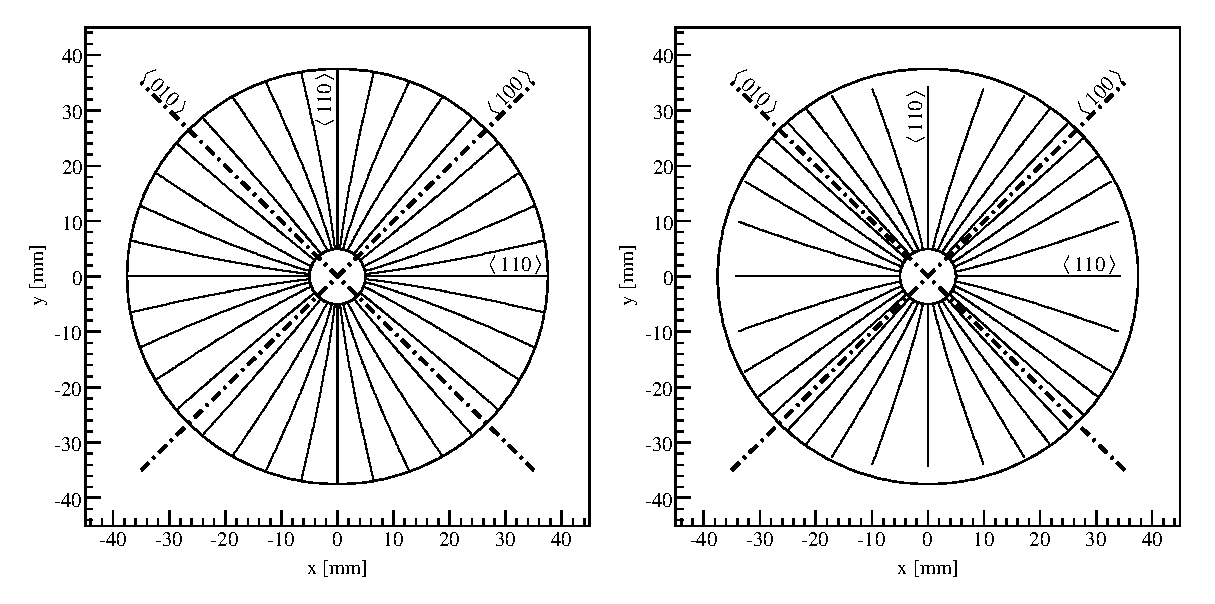
\includegraphics[width=\textwidth]{trjs} 
\caption{Drift trajectories projected on the x-y cross sections of
Siegfried-like detectors: Left, electrons drift inward; Right, holes
drift outward.}
\label{fig:pss:trjs} 
\end{figure} 
 
The trajectories along the crystal axes are straight as explained in
Sec.~\ref{sec:pss:mobi}.  However, they are clearly bent along other
directions.  This causes the different occupancies in different
segments that was shown in Fig.~\ref{fig:ph:mcb}.  The crystal axis
orientation can be deduced by comparing the occupancy distributions of
data and MC.  This will be described in detail in
Chapter~\ref{cha:psa}.
 
 
\section{Raw pulse shapes} 
\label{sec:pss:ps} 
Once the weighting fields and potentials as well as the drift
velocities and trajectories of the charge carriers are known,
Eq.~\ref{eq:det:ramoq} and \ref{eq:det:ramoi} introduced in
Sec.~\ref{sec:det:ramo} can be used to calculate the time development
of the induced charge $Q(t)$ and current $I(t)$ in each electrode (raw
pulses in short), which are shown in Figure~\ref{fig:det:pss}.

 
\section{Effects of electronics} 
\label{sec:pss:dbn} 
The pulses recorded by the DAQ system are quite different from the raw
pulses. Not only their amplitudes but also their shapes are changed
by the electronics. The baseline after a pulse exponentially
decreases to its original level with a time constant $\tau$. The limit
on the bandwidth of the signal transmission through the electronics
cuts off the signal components with frequencies higher than the
limit. Sharp edges in a pulse are hence smeared. Electronic noise may
destroy any detailed structure of a pulse. All these effects need to
be simulated.
 
Figure~\ref{fig:pss:elec} shows a modified pulse after folding in the
decay of the baseline after the pulse, the limited bandwidth and the
noise. The decay time was $5 \mu$s, the cut-off in bandwidth was
10~MHz and the noise level was 5\% of the pulse amplitude. These
values are worse than observed in the tests stands. They were chosen
to clearly demonstrate influence of the effects.
\begin{figure}[htbp] 
\centering 
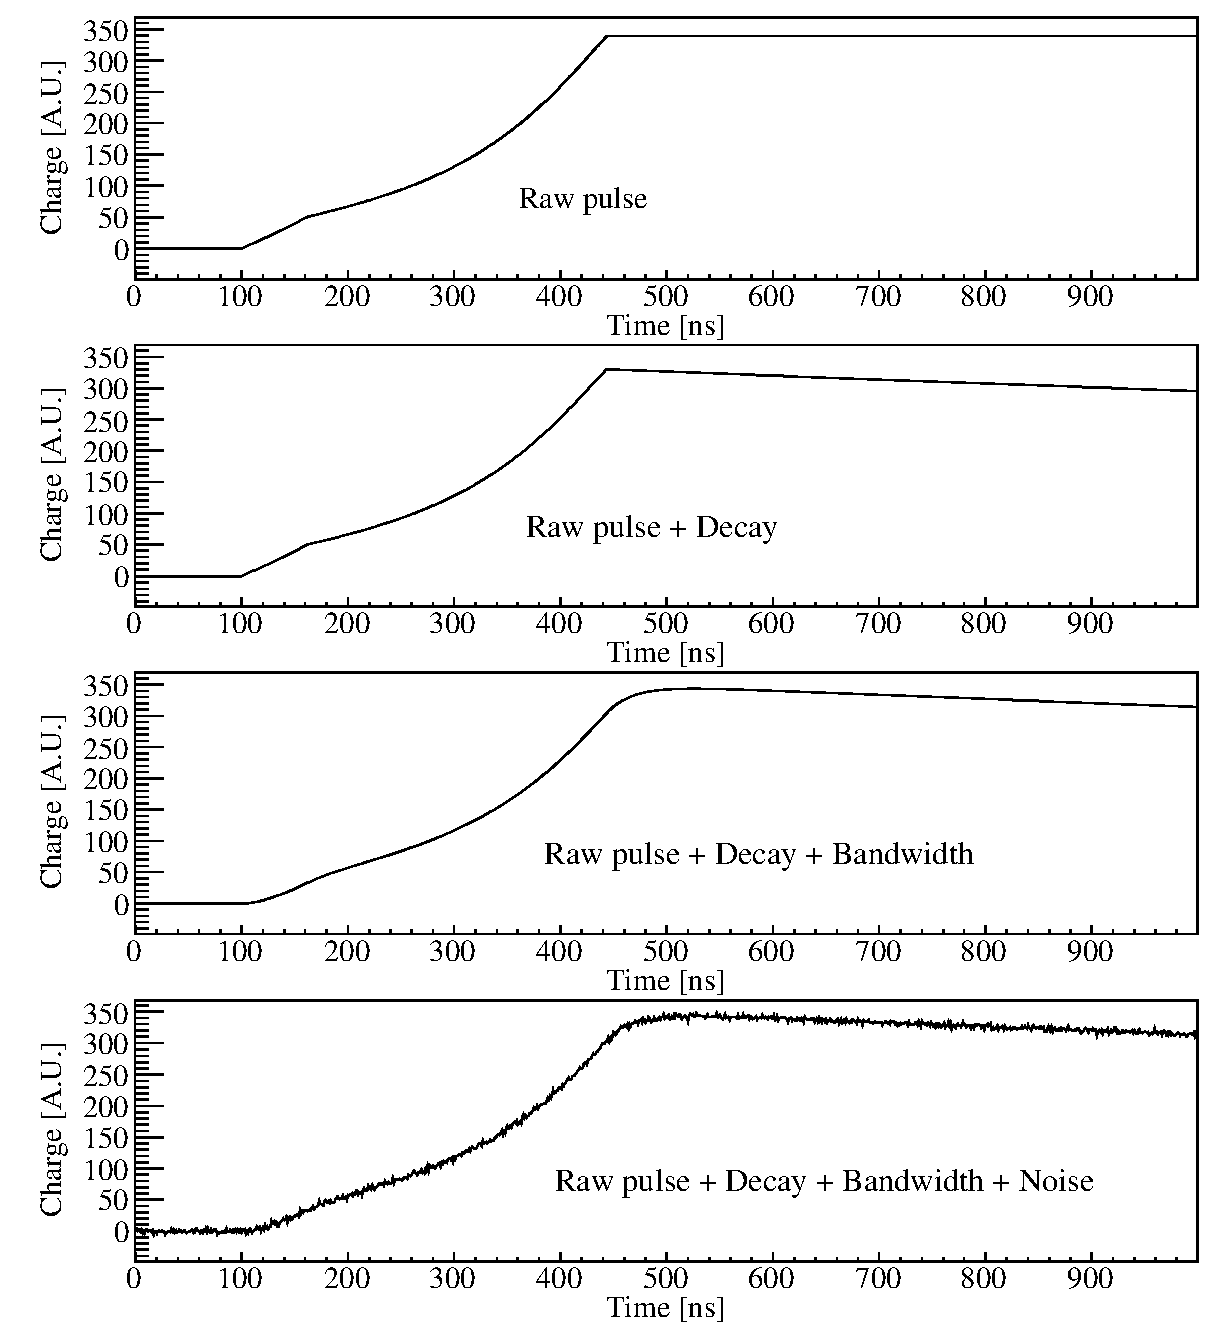
\includegraphics[width=0.7\textwidth]{PSDBN} 
\caption{Modified pulses after folding in the decay of the baseline
after the pulse, the limited bandwidth and the noise.}
\label{fig:pss:elec} 
\end{figure}
 
 
%%% Local Variables: 
%%% mode:latex 
%%% TeX-master: "thesis" 
%%% End: 

\clearpage{\pagestyle{empty}\cleardoublepage}

\chapter{Pulse shape analysis and Event Classification}
\label{cha:psa}
%$Id$



%%% Local Variables:
%%% mode:latex
%%% TeX-master: "thesis"
%%% End:


\chapter{Conclusions and outlook}
\label{cha:con}
\chapter{Summary and outlook} 
\label{cha:con} 
 
The results presented in this thesis can be summarized as follows:
\begin{enumerate}
\item Segmented n-type germanium detectors can be operated stably over long periods submerged in a cryogenic liquid;
\item They can facilitate not only the identification of photon-induced events but also of neutron-induced events;
\item The pulse shapes of segmented detectors can be simulated reliably using basic information about semiconductor-detectors;
\item A novel way to determine the crystal orientation and impurity distribution of a segmented detector was developed.
\end{enumerate}

The work was performed in the context of detector development for Phase~II of the GERDA neutrinoless double beta decay experiment. The results are highly relevant for the realization of this experiment.

\begin{enumerate}

\item Segmented n-type germanium detectors are to be used in Phase~II of GERDA which is based on the idea to submerge detectors in liquid argon to achieve extremely low background levels using the liquid as a shield against external radiation.
\item The background level due to the predicted radioactivity within GERDA can only reach the extremely low level targeted, if both photon-and neutron-induced events are identified with good efficiency.
\item Even though background events are identified very well using segment information, an additional suppression factor of $\approx$\,1.3 for photon-induced events is expected from pulse shape analysis. However, the verification of this expectation is important and impossible without excellent pulse shape simulation.
\item As handling has to be minimized during the production of the GERDA detectors in order to minimize possible contamination, the control measurements should be kept to a minimum. This novel way to determine the crystal orientation needed for pulse shape analysis allows an in-situ measurement of crystal properties during a normal energy calibration inside GERDA cryostat. 
\end{enumerate}

As part of the work presented in this thesis, many tests were made to study segmented germanium detectors and the complete read-out and support system.  The understanding of these novel kind of detectors was enhanced considerably. The operation of the detectors and the tuning of the electronics provides guidelines for the operation of GERDA. This includes monitoring and control software.

The Monte Carlo package, MaGe, used to simulate all aspects of the GERDA experiment, was verified using photon-induced and neutron-induced events. Several problems, especially in the simulation of neutron interactions, were identified and solved. The overall agreement of the Monte Carlo predictions with data taken in the test facilities was very satisfactory.

The detector system including read-out and signal transmission and processing is still being optimized:
\begin{itemize} 
\item the signal transmission inside the cryogenic liquid needs to be further improved to minimize cross-talks and micro-phonic effects;
\item the high voltage distribution into the cryogenic volume has to be improved to allow stable running not only with liquid nitrogen, but also with liquid argon;
\end{itemize}

It is planned to operate three segmented germanium detectors together in liquid argon, providing a test environment as close as possible to the GERDA environment and allowing a large variety of detector studies.

\begin{itemize}
\item Data will be collected with a low energy gamma source placed inside the core of a segmented $n$-type detector. Holes created close to the inner surface of the detector will drift outwards while electrons reach the inner surface almost immediately.  Thus, the drift of the holes can be studied separately.
\item Various surface scans will be performed on at least three different segmented detectors of the same type. This will allow the verification of the pulse shape simulation package with a large variety of data.
\item Several pulse shape analyses will be performed and evaluated using data and Monte Carlo including pulse shape simulation. The potential for background discrimination will be studied in detail.
\end{itemize} 
 
All these studies will rely on the work presented in this thesis and will further the understanding of segmented germanium detectors. The results will provide information for the operation of GERDA and the planning of future germanium based experiments.
 
%%% Local Variables: 
%%% mode:latex 
%%% TeX-master: "thesis" 
%%% End: 

\clearpage{\pagestyle{empty}\cleardoublepage}

\chapter*{Acknowledgement}
\label{cha:ack}
\chapter{Acknowledgements}
\label{cha:ack}




%%% Local Variables:
%%% mode:latex
%%% TeX-master: "thesis"
%%% End:
 
\clearpage{\pagestyle{empty}\cleardoublepage}

\addcontentsline{toc}{chapter}{Bibliography}
\begin{thebibliography}{99}
\bibitem{Sch05} S. Sch\"onert \textit{et al.}, [GERDA Collab.], Nucl. Phys. Proc. Suppl. \textbf{145} (2005) 242.
\bibitem{Pau30}W. Pauli, \emph{Vortr\"age und Aufs\"atze \"uber Physik     und Erkenntnistheorie}, 2. Auflage, Friedr, Vieweg \& Sohn,   Braunschweig/Wiesbaden, (1984) 156.
\bibitem{Fer33}E. Fermi, Ricercha Scient. \textbf{2} (1933) 12.
\bibitem{Fer34}E. Fermi, Z. Phys. \textbf{88} (1934) 161.
%\bibitem{Per33}F. Perrin, Comptes rendues \textbf{197} (1933) 1624.
\bibitem{Lan52}L. M. Langer and R. J. D. Moffat, Phys. Rev.   \textbf{88} (1952) 689.
\bibitem{Cur34}I. Curie and J. F. Joliot, Comptes Rendus \textbf{198}   (1934) 254.
\bibitem{Alv38}L. W. Alvarez, Phys. Rev. \textbf{53} (1938) 606.
\bibitem{Cow56} C. L. Cowan, \textit{et al.}, Science \textbf{124}   (1956) 103.
\bibitem{Rei56}F. Reines and C. L. Cowan, Jr., Nature \textbf{178} (1956) 446.
\bibitem{Dav55}R. Davis Jr., Phys. Rev. \textbf{97} (1955) 766.
\bibitem{Dav56}R. Davis Jr., Bull. American Phys. Soc., Washington   Meeting (1956) 219.
\bibitem{Lee56}T. D. Lee and C. N. Yang, Phys. Rev. \textbf{104}  
(1956) 254.
\bibitem{Wu57}C. S. Wu \textit{et al.}, Phys. Rev. \textbf{105} (1957)  
1413.
\bibitem{Gar57}R. L. Garwin \textit{et al.}, Phys. Rev. \textbf{105}  
(1957) 1415.
\bibitem{Fri57}J. L. Friedman and V. L. Telegdi, Phys. Rev.  
\textbf{105} (1957) 1681.
\bibitem{Lee57}T. D. Lee and C. N. Yang, Phys. Rev. \textbf{105}   (1957) 1671.
\bibitem{Sal57}A. Salam, Nuovo Cimento \textbf{5} (1957) 229.
\bibitem{Lan57}L. Landau, Nucl. Phys. \textbf{3} (1957) 127.
\bibitem{Wey29}H. Weyl, Z. Phys. \textbf{56} (1929) 330.
\bibitem{Gol58}M. Goldhaber \textit{et al.}, Phys. Rev. \textbf{109}   (1958) 1015.
%\bibitem{Rei58}F. Reines and C. L. Cowan, Jr., Phys. Rev. %\textbf{113} (1958) 273.
\bibitem{Gri69}V. Gribov, B. Pontecorvo, Phys. lett. B \textbf{28}   (1969) 493.
\bibitem{Dav64}R. Davis Jr., Phys. Rev. lett. \textbf{12} (1964) 303.
\bibitem{Dav68}R. Davis Jr. \textit{et al.}, Phys. Rev. lett.   \textbf{20} (1968) 1205.
\bibitem{Bah98}J. N. Bahcall, S. Basu and M. H. Pinsonneault, Phys.   Lett. B \textbf{433} (1998) 1.
\bibitem{Wol78}L. Wolfenstein, Phys. Rev. D \textbf{17} (1978) 2369.
\bibitem{Mik86}S. P. Mikheyev, A. Yu. Smirnov, Yad. Fiz. \textbf{42}  
(1985) 1441; Nuovo Cimento C \textbf{9} (1986) 17.
\bibitem{Hir89}K. S. hirata \textit{et al.}, [Kamiokande Collab.],   Phys. Rev. Lett. \textbf{63} (1989) 16.
\bibitem{Aba91}A. I. Abazov \textit{et al.}, [SAGE Collab.], Phys.   Rev. Lett. \textbf{67} (1991) 3332.
\bibitem{Ans92}P. Anselmann \textit{et al.}, [Gallex Collab.], Phys.   Lett. B \textbf{285} (1992) 376.
\bibitem{Ahm01}Q. R. Ahmad \textit{et al.}, [SNO Collab.], Phys. Rev.   Lett. \textbf{87} (2001) 071301.
\bibitem{Fuk01}S. Fukuda \textit{et al.}, [Kamiokande Collab.], Phys.   Rev. Lett. \textbf{86} (2001) 5651.
\bibitem{Hai86}T. J. Haines \textit{et al.}, [IMB Collab.], Phys. Rev.  
Lett. \textbf{57} (1986) 1986.
\bibitem{Hir88}K. S. Hirata \textit{et al.}, [Kamiokande Collab.],  
Phys. lett. B \textbf{205} (1988) 416
\bibitem{Fuk94}Y. Fukuda \textit{et al.}, [Kamiokande Collab.], Phys.  
Lett. B \textbf{335} (1994) 237.
\bibitem{Fuk98}Y. Fukuda \textit{et al.}, [Kamiokande Collab.], Phys.  
Rev. Lett. \textbf{81} (1998) 1562; Phys. Lett. B, \textbf{436}  
(1998) 33.
\bibitem{Kam03}Araki T \textit{et al.}, [KamLAND Collab.], Phys. Rev.   Let. \textbf{90} (2003) 021802.
\bibitem{Kam08}S. Abe \textit{et al.}, [KamLAND Collab.],   arXiv:hep-ex/0801.4589v3.
\bibitem{Cho03}M. Apollonio \textit{et al.}, [Chooz Collab.], Eur.   Phys. J. C \textbf{27} (2003) 331.
\bibitem{Koz03}Yu. Kozlov, L. Mikaelyan, V. Sinev, Phys. Atom. Nucl.   \textbf{66} (2003) 1934; Yad. Fiz. \textbf{66} (2003) 1986.
\bibitem{Dbc06}F. Ardellier \textit{et al.}, arXiv:hep-ex/0606025v4.
\bibitem{Day07}Daya Bay Collab. arXiv:hep-ex/0701029v1.
\bibitem{Ren08}S. Kim, NuFact 07. AIP Conf. Proc. \textbf{981} (2008)   205.
\bibitem{K2K06}M. H. Ahn \textit{et al.}, [K2K Collab.], Phys. Rev. D   \textbf{74} (2006) 072003.
\bibitem{Min06}D. G. Michael \textit{et al.}, [MINOS Collab.],   Phys.Rev.Lett. \textbf{97} (2006) 191801.
\bibitem{Ope06}R Acquafredda \textit{et al.}, [OPERA Collab.], New J. Phys. \textbf{8}, (2006) 303.
\bibitem{Kar03}B. Armbruster \textit{et al.}, [KARMEN Collab.], Phys. Rev. Lett. \textbf{90} (2003) 181804.
\bibitem{Dod06}S. Dodelson, A. Melchiorri, A. Slosar, Phys. Rev. Lett.   \textbf{97} (2006) 04301.
\bibitem{Agu07}A. A. Aguilar-Arevalo \textit{et al.}, [MiniBooNE   Collab.], Phys. Rev. Lett. \textbf{98} (2007) 231801.
\bibitem{T2K05}Y. Oyama, arXiv:hep-ex/0512041v2.
\bibitem{Nov05}D. S. Ayres \textit{et al.}, [NOvA Collab.],   arXiv:hep-ex/0503053.
\bibitem{PDG08}C. Amsler \textit{et al.}, [Particle Data Group], Phys. Lett. B \textbf{667} (2008) 1.
\bibitem{Oli02}K. A. Olive arXiv:astro-ph/0202486.
\bibitem{Str05}A. Strumia and F. Vissani, arXiv:hep-ph/0503246v1.
\bibitem{Fog08}G.L. Fogli \textit{et al.}, arXiv:hep-ph/0805.2517v2.
\bibitem{Pla05}Planck Collab., ESA-SCI(2005)-1. Version 2.
\bibitem{Mai99}C. Weinheimer \textit{et al.}, Phys. Lett. B \textbf{460} (1999) 219.
\bibitem{Tro99}V. M. Lobashev \textit{et al.}, Phys. Lett. B \textbf{460} (1999) 227.
\bibitem{Kat01}A. Osipowicz \textit{et al.}, arXiv:hep-ex/0109033.
\bibitem{Mar05}A. Monfardini \textit{et al.}, arXiv:hep-ex/0509038.
\bibitem{Cuo08}C. Arnaboldi \textit{et al.}, [CUORICINO Collab.], arXiv:0802.3439v1.
\bibitem{Hei04}H. V. Klapdor-Kleingrothaus \textit{et al.}, Phys. Lett. B \textbf{586} (2004) 198.
\bibitem{Fog07}G. L. Fogli \textit{et al.}, Phys. Rev. D \textbf{75} (2007) 053001.
\bibitem{Ass96}K. Assamagan \textit{et al.}, Phys. Rev. D \textbf{53} (1996) 6065.
\bibitem{Num20}NuMass Collab. http://www.hep.umn.de/numass.
\bibitem{Yos07} M. Yoshimura, arXiv:hep-ph/0611362v4.
\bibitem{Fuj80} K. Fujikawa and R. Shrock, Phys. Rev. Lett. \textbf{45} (1980) 963.
\bibitem{Lim88}C. S. Lim and W. J. Marciano, Phys. Rev. D \textbf{37} (1988) 1368.
\bibitem{Akh88}E. Kh. Akhmedov, preprint IAE-4568/1 (1988).
\bibitem{Gri02}W. Grimus \textit{et al.}, Nucl. Phys. B \textbf{648} (2002) 376.

% Chapter 3
\bibitem{Rod07}V. Rodin \textit{et al.}, Nucl.Phys. A \textbf{766}  
(2006) 107. [Erratum A \textbf{793} (2007) 213]
\bibitem{Cal06}A. Caldwell, K. Kr\"oninger, Phys. Rev. D \textbf{74} (2006) 092003. [arXiv:physics/0608249]
\bibitem{Mut90} K. Muto \textit{et al.}, Z. Phys. A \textbf{334}   (1989) 187; Z. Phys. A \textbf{339} (1991) 435; Europhys. Lett.   \textbf{13} (1990) 31.
\bibitem{Sim08}F. Simkovic \textit{et al.}, arXiv:0710.2055v3 (2 April   2008).
\bibitem{Cau08}E. Caurier \textit{et al.}, Eur. Phys. J. A \textbf{36}
  (2008) 195. [arXiv:0709.0277]
\bibitem{Oga04} I. Ogawa \textit{et al.}, Nucl. Phys. A \textbf{730}   (2004) 215.
\bibitem{Ume06}S. Umehara \textit{et al.}, J. of Phys.: Conf. Series \textbf{39} (2006) 356.
\bibitem{Zde05} Yu. G. Zdesenko \textit{et al.}, Astropart. Phys. \textbf{23} (2005) 249.
\bibitem{Aal02}C. E. Aalseth \textit{et al.}, [IGEX Collab.] Phys. Rev. D \textbf{65} (2002) 092007. [arXiv:hep-ex/0202026]
\bibitem{Gai03} R. Gaitskell \textit{et al.}, [Majorana Collab.] arXiv:nucl-ex/0311013.
\bibitem{Aal04}C. E. Aalseth \textit{et al.}, [Majorana Collab.] Phys. Atom. Nucl. \textbf{67} (2004) 2002. [Yad. Fiz. \textbf{67} (2004) 2025] [arXiv:hep-ex/0405008]
\bibitem{Zub01} K. Zuber, Phys. Lett. B \textbf{519} (2001) 1.
\bibitem{Ell02} S. Elliot, P. Vogel, Ann. Rev. Nucl. Part. Sci.   (2002).
\bibitem{Kie03} H. Kiel \textit{et al.}, Nucl. Phys. A \textbf{723} (2003) 499.
\bibitem{Pre04}E. Previtali \textit{et al.}, Nucl. Instr. and Meth. in Phys. Res. A \textbf{518} (2004) 256258.
\bibitem{Arn04}C. Arnaboldi \textit{et al.}, Nucl. Instr. and Meth. in Phys. Res. A \textbf{518} (2004) 775798.
\bibitem{Ard05}R. Ardito \textit{et al.}, arXiv:hep-ex/0501010.
\bibitem{Arn08}C. Arnaboldi \textit{et al.}, arXiv:0802.3439v1.
\bibitem{Avi05}F T Avignone III, G S King III and Yu G Zdesenko, New J. of Phys. \textbf{7} (2005) 6.
\bibitem{Dan00}F. A. Danevich \textit{et al.}, Phys. Rev. C \textbf{62} (2000) 045501.
\bibitem{Dan03}F. A. Danevich \textit{et al.}, Phys. Rev. C \textbf{68} (2003) 035501.
\bibitem{Bel00}G. Bellini \textit{et al.}, Phys. Lett. B \textbf{493} (2000) 216.
\bibitem{Bel01}G. Bellini \textit{et al.}, Eur. Phys. J. C \textbf{19} (2001) 43.
\bibitem{Arp08}C. Arpesella \textit{et al.}, [Borexino Collab.], Phys.   Lett. B \textbf{658}, (2008) 101.
\bibitem{Lue98}R. Luescher \textit{et al.}, Phys. Lett. B \textbf{434} (1998) 407.
\bibitem{Aki05}D. Akimov \textit{et al.}, Nucl. Phys. Proc. Suppl. \textbf{138} (2005) 224.
\bibitem{Kim05}Y. D. Kim, [for XMASS Collab.], 	Phys. of Atomic Nuclei, \textbf{69} (2006) 1970.
\bibitem{Zub07}K. Zuber, [for SNO+ Collab.], AIP Conf. Proc. \textbf{942} (2007) 101.
\bibitem{Ste98}I. \u{S}tekl \textit{et al.}, Czech. J. Phys. \textbf{48} (1998) 249.
\bibitem{Ste00}I. \u{S}tekl \textit{et al.}, Czech. J. Phys. \textbf{50} (2000) 553.
\bibitem{Ste06}I. \u{S}tekl \textit{et al.}, Czech. J. Phys. \textbf{56} (2006) 505.
\bibitem{Das91}D. Dassi\'{e} \textit{et al.}, Nucl. Instr. and Meth. A \textbf{309} (1991) 465.
\bibitem{Arn95}R. Arnold \textit{et al.}, Nucl. Instr. Meth. A \textbf{354} (1995) 338.
\bibitem{Arn05}R. Arnold \textit{et al.}, Nucl. Inst. Meth. A \textbf{536} (2005) 79.
\bibitem{Arn07}R. Arnold \textit{et al.}, Nucl. Phys. A \textbf{781} (2007) 209.
\bibitem{Sne08}SuperNEMO homepage: http://nemo.in2p3.fr/supernemo/
\bibitem{Nak06}H. Nakamura \textit{et al.}, J. Phys. Conf. Ser. \textbf{39} (2006) 350.
\bibitem{Ish05}N. Ishihara \textit{et al.}, Nucl. Phys. B Proc. Suppl. \textbf{143} (2005) 549.
\end{thebibliography}

%%% Local Variables:
%%% mode:latex
%%% TeX-master: "thesis"
%%% End:



\end{document}
